\documentclass[]{interact}

\usepackage[utf8]{inputenc}
\usepackage[T1]{fontenc}
\usepackage{multirow}
\usepackage{xcolor}
\usepackage{textcomp}
\usepackage{array}
\usepackage{float}
\usepackage{algorithm}
\usepackage{algpseudocode}
\usepackage{comment}
\usepackage{url}
\usepackage{csquotes}

\usepackage[
  backend=biber,
  style=apa,
  natbib=true,
  sortcites=true,
  sorting=nyt,
  doi=true,
  url=true,
  isbn=false
]{biblatex}
\DeclareLanguageMapping{english}{english-apa}
\addbibresource{jit-references.bib}
\setlength\bibhang{12pt}
\AtBeginBibliography{\fontsize{10}{12}\selectfont}

\raggedbottom

\begin{document}

\title{POMA: A Parallel Multi-Agent Orchestration for Vietnamese Table Question Answering}

\author{
\name{Nguyen Dinh Khoi\textsuperscript{*}\thanks{Email: 23520774@gm.uit.edu.vn. ORCID: \protect\url{https://orcid.org/0009-0001-6385-3444}} and
Dang Van Thin\textsuperscript{*}\thanks{CONTACT Dang Van Thin. Email: thindv@uit.edu.vn}}
\affil{\textsuperscript{*}University of Information Technology - Vietnam National University Ho Chi Minh City, Ho Chi Minh City, Vietnam}
}

\maketitle

\begin{abstract}
Vietnamese Table Question Answering requires models to interpret semi-structured evidence, perform heterogeneous reasoning, recognize unsupported questions, and produce concise evaluation-compatible answers. Although large language models have demonstrated strong reasoning capabilities, direct prompting assigns evidence selection, reasoning, answerability assessment, and answer formatting to a single generation step, making the process vulnerable to grounding and output errors. To address these limitations, this paper proposes POMA, a training-free Parallel Multi-Agent Orchestration framework that predicts canonical question hints, refines each question into a structured query, deterministically routes it to appropriate specialist agents, executes the selected agents in parallel, and normalizes their outputs into final answer variants. POMA is evaluated on the official 992-instance Open-ViTabQA test split using Qwen3 8B and matched zero-shot, task-decomposition, chain-of-thought, and few-shot baselines. It achieves 80.24\% Exact Match, 88.23\% F1, 86.07\% ROUGE-1, and 84.50\% METEOR, exceeding the strongest matched few-shot baseline by 13.10, 9.59, 11.89, and 12.20 points, respectively. These results demonstrate the value of modular multi-agent orchestration for Vietnamese Table QA while highlighting remaining trade-offs in answerability and inference efficiency.
\end{abstract}

\begin{keywords}
Vietnamese Table QA; large language models; multi-agent systems; prompt engineering; Open-ViTabQA
\end{keywords}

\section{Introduction}\label{sec:introduction}

Question answering over tables is an important interface for accessing structured and semi-structured information. A user who asks a natural-language question about a table expects the system to identify the relevant schema, retrieve or derive supporting evidence, and return a concise answer without requiring SQL, spreadsheet formulas, or manual inspection. This setting is challenging because tables often encode hierarchy, grouping, aggregation, and implicit relations that are not visible from a single cell. The challenge is more pronounced in Vietnamese, where question words may appear at the beginning, middle, or end of a sentence, answer forms are often short and evaluation-sensitive, and public benchmarks remain scarce. Open-ViTabQA is the first large Vietnamese benchmark designed for table question answering over open-domain Wikipedia tables \citep{openvitabqa2025}. It contains 9,911 question-answer pairs derived from 329 tables across 41 domains and uses a table-disjoint train/development/test split to reduce table-level leakage across partitions. The dataset covers diverse question types, including wh-questions, yes/no questions, list queries, mathematical reasoning, multi-condition filtering, and unanswerable cases whose correct answer is the literal string Null, indicating that the table lacks sufficient evidence.

Despite recent progress in large language models, Vietnamese Table QA remains difficult because direct prompting places heterogeneous operations into one generation step. We use direct prompting to refer to single-agent prompt baselines that ask one model call to solve the task from the serialized table and question. A model must interpret the question, recover the relevant table structure, select evidence, perform reasoning when needed, decide whether the question is answerable, and produce the expected surface form. These requirements are particularly demanding on Open-ViTabQA, where 55.6\% of tables contain merged cells, roughly 59\% of questions require complex multi-hop reasoning, and about 10\% involve reasoning over multiple entities. Direct prompting can therefore fail in two answerability directions: it may generate a plausible answer when the table does not support one, or it may return Null even though sufficient evidence is present. It can also count over the wrong subset of rows, treat a multi-condition query as a simple lookup, or produce a correct value in an evaluation-incompatible form. Chain-of-thought and few-shot prompting can improve reasoning, but they still leave one response responsible for all of these subproblems.

To address this gap, we propose POMA, Parallel Multi-Agent Orchestration, a prompt-based multi-agent framework for Vietnamese Table QA. POMA is based on the observation that Open-ViTabQA question types correspond to different reasoning demands. Rather than using one prompt for all cases, POMA predicts canonical hints from the question and table, refines the question into a structured representation, deterministically routes the instance to specialist agents, executes the selected specialists in parallel, and normalizes their outputs into final answer variants. The framework does not retrain the model, replace the table parser, or introduce arbitrary runtime agents; routing is controlled by a fixed canonical hint vocabulary: What, Where, Who, When, Why, How, Yes \& No, List, Mathematical Reasoning, and Multiple Conditions.

Our contributions are twofold. First, we develop POMA, a training-free multi-agent system for Vietnamese Table QA that integrates question-hint prediction, structured question refinement, deterministic specialist routing, parallel reasoning, and answer normalization. Second, we conduct a comprehensive evaluation and analysis on Open-ViTabQA by comparing POMA with matched prompting baselines and examining its performance across question types, answerability, table structures, hint sources, answer normalization, and inference efficiency.

\section{Related Work}\label{sec:related}

\subsection{Table Question Answering}

Table question answering has been studied through semantic parsing, table-aware neural encoders, text-table hybrid reasoning, and more recently LLM prompting. Early semantic parsing datasets and systems such as WikiTableQuestions, WikiSQL, Spider, and SQA map a question into executable logical forms or SQL-like programs over structured or semi-structured tables \citep{pasupat-liang-2015-compositional,zhong-etal-2017-seq2sql,yu-etal-2018-spider,iyyer-etal-2017-search}. Related table reasoning datasets such as TabFact, HybridQA, OTT-QA, FeTaQA, and HiTab broaden the setting to fact verification, hybrid table-text reasoning, free-form answers, and hierarchical tables \citep{chen-etal-2020-tabfact,chen-etal-2020-hybridqa,chen-etal-2021-ottqa,nan-etal-2022-fetaqa,cheng-etal-2022-hitab}. These resources show that table QA is not only a cell lookup task but also a reasoning task involving schema alignment, aggregation, multi-hop evidence, and answer form control.

Table-specialized encoders and pretraining methods attempt to represent table structure more directly. TAPAS extends BERT-like modeling to weakly supervised table parsing, TaBERT jointly pretrains over text and tables, TAPEX uses synthetic SQL execution as a pretraining signal, and OmniTab combines natural and synthetic supervision for few-shot table QA \citep{herzig-etal-2020-tapas,yin-etal-2020-tabert,liu-etal-2022-tapex,jiang-etal-2022-omnitab}. Other neural approaches, including row-column intersection modeling, emphasize explicit table-cell grounding \citep{glass-etal-2021-capturing}. These models have improved performance on several table benchmarks, yet their context limits and training assumptions can be problematic for long, irregular, open-domain tables. POMA focuses on an inference-time prompt-based setting, but it inherits the same need to preserve row-column evidence and avoid unconstrained free-form generation.

\subsection{Vietnamese Question Answering and Open-ViTabQA}

Vietnamese NLP remains comparatively low-resource relative to English. Vietnamese question answering requires sensitivity to tone marks, word segmentation, flexible word order, and question-particle placement. General Vietnamese language resources and models such as UIT-ViQuAD, PhoBERT, ViT5, and ViNLI have supported progress in machine reading comprehension, Vietnamese representation learning, generation, and natural language inference \citep{nguyen-etal-2020-vietnamese,nguyen-nguyen-2020-phobert,phan-etal-2022-vit5,huynh-etal-2022-vinli}. Open-ViTabQA addresses a major gap by introducing a Vietnamese Table QA benchmark built from Wikipedia tables \citep{openvitabqa2025}. The dataset paper reports strong baselines from Vietnamese pretrained models, table-aware models, and prompting LLMs, but also shows a large gap to human performance. In particular, models struggle with merged-cell tables, abstract answers, mathematical operations, and unanswerable questions. POMA uses Open-ViTabQA as the target benchmark and treats its hint taxonomy as an important signal for routing and specialization.

\subsection{LLM Prompting for Structured Data Reasoning}

LLMs can reason over serialized structured data using zero-shot, few-shot, chain-of-thought (CoT), self-consistency, or tool-like decomposition \citep{brown-etal-2020-language,wei-etal-2022-chain,wang-etal-2023-selfconsistency,yao-etal-2023-react}. Recent table-oriented LLM methods explicitly study whether language models can understand serialized tables, bind natural-language questions to symbolic programs, decompose table evidence, or evolve the table itself through a reasoning chain \citep{sui-etal-2024-table,cheng-etal-2023-binder,ye-etal-2023-dater,wang-etal-2024-chain}. Prompting avoids retraining and enables rapid adaptation across model backbones, including commercial and open-weight LLMs \citep{openai-2024-gpt4,dubey-etal-2024-llama,qwen-team-2025-qwen3}. However, prompting over tables has two recurring failure modes. First, the model may not preserve structural grounding when the flattened table is long or irregular. Second, even when the model identifies the right evidence, it may output an answer in a form that is semantically acceptable but evaluation-incompatible. These issues are acute in Open-ViTabQA because the expected answers are concise and Vietnamese surface forms vary.

\subsection{Multi-agent LLM Systems}

Multi-agent LLM systems decompose a problem across role-specialized agents, reviewers, voters, or verifiers. Self-refinement and reflexive feedback show that LLM outputs can be improved through iterative critique, while AutoGen and MetaGPT demonstrate broader multi-agent conversation and role assignment patterns \citep{madaan-etal-2023-selfrefine,shinn-etal-2023-reflexion,wu-etal-2023-autogen,hong-etal-2024-metagpt}. Recent surveys further characterize multi-agent LLM systems as a family of inference-time coordination methods \citep{guo-etal-2024-multiagent}. Such systems can improve robustness by encouraging independent reasoning paths, but they also increase orchestration complexity and inference cost.

Recent work has applied multi-agent coordination directly to tabular reasoning. CoAgt organizes inference as a sequential chain in which each agent builds on the output produced by its predecessor \citep{alrayzah-alqhtani-2025-coagt}. Chain-of-Query (CoQ) combines multi-agent collaboration with intermediate SQL-aided queries for table understanding and question answering \citep{sui-etal-2025-coq}. These systems illustrate sequential and query-assisted coordination, respectively. POMA instead predicts canonical hints, routes each question deterministically, executes the selected specialists in parallel, and normalizes their outputs into evaluation-ready answer variants.

\subsection{Routing, specialization, and answer normalization}

Routing and specialization are common design patterns for complex QA systems. A router can decide whether a question should be answered by a retriever, calculator, verifier, or generator. In POMA, routing is deterministic once canonical hints are known. The more task-specific component is answer normalization. For Vietnamese Table QA, this module must handle yes/no variants, numeric units, date forms, list permutations, ranking expressions, and Null predictions. We treat answer normalization as a first-class stage because exact-match and overlap metrics such as R1 and MET are sensitive to surface form and semantic equivalence \citep{lin-2004-rouge,banerjee-lavie-2005-meteor}.

\section{Methodology}\label{sec:method}

This section formalizes Vietnamese Table QA on Open-ViTabQA and presents the proposed POMA framework. POMA is an inference-time orchestration method: it does not update model parameters, add a task-specific encoder, or require gold question-type annotations at test time. Given a flattened table and a Vietnamese question, the framework predicts canonical hints, refines the question into a structured query, routes the instance to specialist agents, executes the selected agents in parallel, and normalizes their outputs into evaluation-ready answer variants. Figure~\ref{fig:poma-pipeline} illustrates the overall pipeline.

\begin{figure}[!t]
\centering
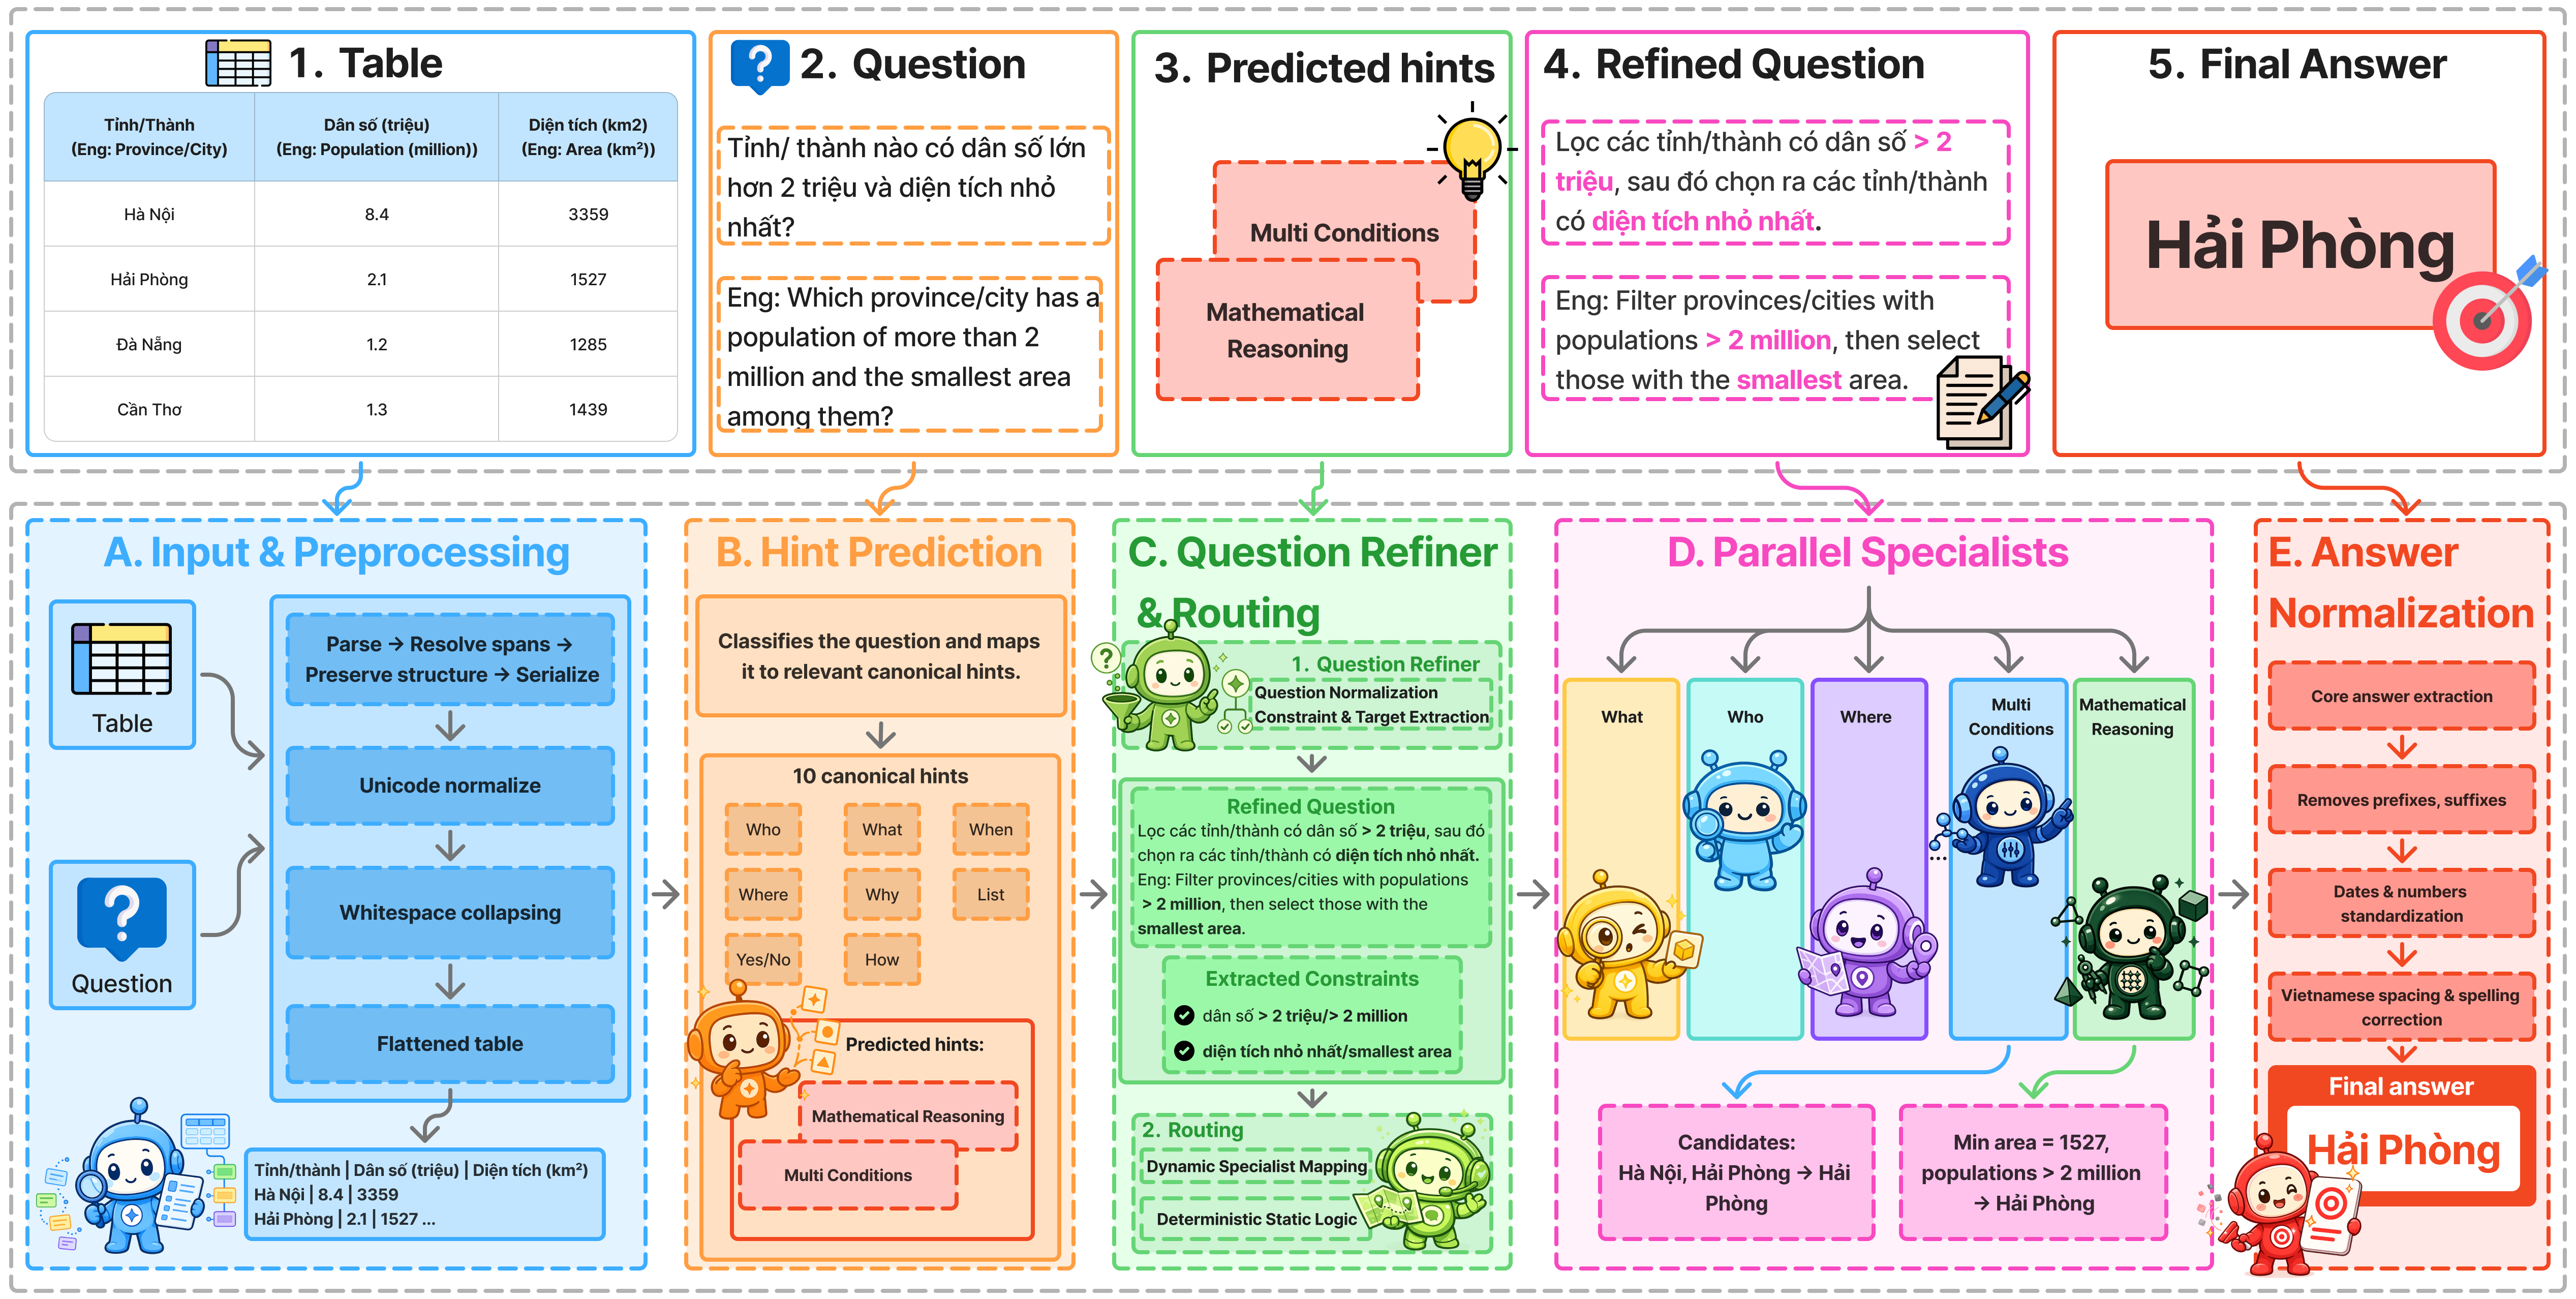
\includegraphics[width=\linewidth]{figures/pipeline.png}
\caption{Architecture of POMA. The system receives a Vietnamese question and a flattened table. hint predictor predicts canonical hints, question refiner produces a structured query without answering, and router deterministically maps canonical hints to specialist agents. Routed specialists execute in parallel and return answer, evidence, confidence, and reason fields. answer normalization then consolidates raw outputs and generates evaluation-ready surface variants, including Null when appropriate.}\label{fig:poma-pipeline}
\end{figure}

\subsection{Problem Formulation}

Let $D=\{(T_i,q_i,y_i)\}_{i=1}^{N}$ denote a set of Vietnamese Table QA instances, where $T_i$ is a table, $q_i$ is a Vietnamese natural-language question, and $y_i$ is the reference answer. In Open-ViTabQA, an answer may be a grounded textual value supported by the table or the literal string Null when the table does not contain sufficient evidence. unanswerable questions are those whose gold answer is Null because the table lacks sufficient evidence. We therefore define the output space as $y_i \in \mathcal{Y}_{\mathrm{ans}} \cup \{\text{Null}\}$, where $\mathcal{Y}_{\mathrm{ans}}$ denotes the set of table-grounded answers.

Before inference, each table $T_i$ is converted into a flattened textual representation $\tilde{T}_i$. Given the input pair $(\tilde{T}_i,q_i)$, POMA implements an inference function $f_{\theta}$ using a frozen LLM backbone $\theta$: $\hat{Y}_i=f_{\theta}(\tilde{T}_i,q_i)$, where $\hat{Y}_i=\{\hat{y}_{i}^{1},\ldots,\hat{y}_{i}^{K}\}$ is a set of $K$ candidate answer variants produced after answer normalization. The evaluation script compares this candidate set with the gold answer $y_i$ and selects the best-matching candidate for metrics such as EM, F1, R1, and MET. This formulation is suitable for Vietnamese Table QA because correct answers may have multiple acceptable surface forms, while unanswerable questions require an explicit Null prediction.

\subsection{Table Representation}

POMA follows the Flatten V1 representation used in Open-ViTabQA \citep{openvitabqa2025}. Let $g(\cdot)$ denote the table-flattening function. For each raw HTML table $T$, the serialized input is defined as $\tilde{T}=g(T)$. The process first resolves the table into a rectangular logical grid by distinguishing header cells (\texttt{<th>}) from data cells (\texttt{<td>}). Values covered by \texttt{rowspan} or \texttt{colspan} are propagated to every logical position that they span, and missing positions are padded with empty strings. The text of every cell is then normalized by collapsing repeated whitespace and trimming its boundaries.

The resolved grid is serialized row by row. If the expanded table has $m$ logical rows, then $\tilde{T}=[\ell_0,\ell_1,\ldots,\ell_{m-1}]$, where each $\ell_i$ is one logical row. Thus, the list contains the logical rows of the table after merged-cell expansion. The cells in a row are joined using the delimiter \texttt{|}; a cell that functions as a row or column header receives the suffix \texttt{<header>}. Consequently, multi-level headers, row labels, and data values remain in their original row-column arrangement after conversion to text. POMA does not modify this parser during inference. All downstream modules therefore operate over the same row-oriented Flatten V1 representation rather than over isolated cell records, preserving the structural evidence needed for table-grounded reasoning.

\subsection{Hint Predictor}

The hint predictor serves as the first reasoning-oriented component in POMA. Given a Vietnamese question and its flattened table context, it identifies one or more canonical hint labels that describe the expected reasoning behavior of the instance. Let $\mathcal{H}$ denote the fixed Open-ViTabQA hint vocabulary, which includes What, Where, Who, When, Why, How, YesNo, List, MathematicalReasoning, and MultiConditions. The hint predictor $P_{\theta}$ maps the input pair $(\tilde{T},q)$ to a non-empty subset of canonical hints, written as $\hat{H}=P_{\theta}(\tilde{T},q)$ with $\hat{H}\subseteq\mathcal{H}$.

This constrained prediction space prevents the system from creating arbitrary task labels and ensures that all subsequent modules operate over a shared, interpretable set of reasoning categories. The predicted hints provide the initial control signal for question refinement and routing. In this way, POMA can operate at test time without relying on dataset-provided annotations. For analysis, we additionally report a dataset-hint diagnostic setting in which gold annotated hints replace predicted hints, written as $\hat{H}_{\mathrm{gold}}=H^{\mathrm{gold}}$. This diagnostic comparison allows us to examine whether the hint predictor provides an effective runtime substitute for dataset annotations and whether predicted hints contribute positively to the overall reasoning pipeline.

\subsection{Question Refiner}

The question refiner converts the raw question into a structured query while preserving its original meaning. Given the question $q$ and predicted hint set $\hat{H}$, the refiner $R_{\theta}$ produces a structured representation $s=R_{\theta}(q,\hat{H}), \quad s=(\bar{q},t,c)$. Here, $\bar{q}$ is the normalized question, $t$ is the target information being requested, and $c$ is the set of constraints that must be satisfied. These constraints may include entity filters, temporal restrictions, comparisons, negation, counting requirements, or multi-condition logic.

The refiner is explicitly instructed not to answer the question. Its role is to make the intent of the query more explicit before evidence selection begins. This separation is important because direct prompting often entangles question interpretation and answer generation in a single step. By isolating intent structuring from answer production, POMA reduces ambiguity for downstream specialists and provides a more stable interface for routing.

\subsection{Hint-Based Router}

The router is a deterministic component that maps canonical hints to specialist agents. Let $\mathcal{A}$ denote the set of available specialists: $\mathcal{A}=\{a_{\text{What}},a_{\text{Where}},a_{\text{Who}},a_{\text{When}},a_{\text{Why}},a_{\text{How}},a_{\text{YesNo}},a_{\text{List}},a_{\text{Math}},a_{\text{Multi}}\}$. The router implements a fixed mapping function $\rho:\mathcal{H}\rightarrow \mathcal{A}$. Given the predicted hint set $\hat{H}$, the selected agent set is $\hat{A}=\{\rho(h)\mid h\in\hat{H}\}$.

Because $\rho$ is deterministic, routing behavior is reproducible once the hints are fixed. The router does not call an LLM, create new agents, or introduce ad hoc tools. This design keeps the orchestration interpretable: each activated specialist can be traced back to a predicted reasoning category.

\subsection{Parallel Specialist Agents}

Each specialist is a prompt-conditioned reasoning module associated with one canonical question category. Given the flattened table $\tilde{T}$ and the refined query $s$, each selected specialist $a_k\in\hat{A}$ produces a structured result $z_k=a_k(\tilde{T},s), \quad z_k=(\alpha_k,e_k,\gamma_k,r_k)$. Here, $\alpha_k$ is the specialist's answer candidate, $e_k$ is the supporting evidence, $\gamma_k$ is a confidence signal, and $r_k$ is a short explanation of the specialist's reasoning. The answer candidate may be Null when the specialist cannot find sufficient table evidence.

\begin{table}[!t]
\caption{Specialist agents and primary roles in POMA.}\label{tab:hint-specialist}
\begin{tabular*}{\textwidth}{@{\extracolsep{\fill}}p{0.36\textwidth}p{0.58\textwidth}}
\toprule
\textbf{Specialist} & \textbf{Primary role} \\
\midrule
WhatAgent & Extract short surface-form table values, attributes, or entities when direct evidence is available. \\
WhereAgent & Extract explicitly stated locations, places, or positions without adding unsupported description. \\
WhoAgent & Identify people or human subjects satisfying the conditions, including multiple matches or table-grounded negative answers. \\
WhenAgent & Extract time points or time intervals, including simple durations when the table provides enough temporal evidence. \\
WhyAgent & Extract table-grounded reasons or causes only when the table explicitly supports the explanation. \\
HowAgent & Extract methods, procedures, manners, states, or relations only when the table directly describes them. \\
YesNoAgent & Verify a proposition against the table and return a Vietnamese yes/no label or Null. \\
ListAgent & Enumerate all items satisfying the conditions, with sorting, deduplication, or an explicit no-match answer when supported. \\
MathematicalReasoningAgent & Lock relevant rows and columns, then perform counting, arithmetic, comparison, ranking, duration reasoning, or numeric lookup. \\
MultiConditionsAgent & Combine multiple row, column, or cell conditions with the correct logical semantics before producing the final answer. \\
\bottomrule
\end{tabular*}
\end{table}

When multiple hints are active, POMA executes the corresponding specialists in parallel: $Z=\{z_k\mid a_k\in\hat{A}\}$. Parallel execution is useful because Open-ViTabQA questions often combine reasoning demands. For example, a list question may also require temporal filtering, a yes/no question may require multi-condition verification, and a mathematical question may require row selection before computation. Running multiple specialists allows POMA to collect complementary hypotheses before final consolidation. If one specialist fails while others succeed, that specialist can abstain without terminating the entire pipeline.

\subsection{Answer Normalization}

The final module consolidates specialist outputs into evaluation-ready answer variants. Let $N_{\theta}$ denote the answer normalization function. Given the set of specialist results $Z$, the final prediction is $\hat{Y}=N_{\theta}(Z)$. The answer normalization module removes redundant reasoning traces, standardizes whitespace, regularizes list separators, canonicalizes Vietnamese yes/no forms, and preserves Null when the evidence is insufficient. The goal is not to introduce new reasoning but to convert the specialist outputs into concise answer forms that match the benchmark's evaluation format.

This step is important because Vietnamese Table QA answers are often short and surface-sensitive. A raw specialist response may contain the correct value together with an explanation, or it may express the same polarity using a longer phrase than the reference answer. By producing a compact set of variants, answer normalization improves alignment between the reasoning result and automatic evaluation while preserving the table-grounded content selected by the specialists.


\section{Experimental Setup}\label{sec:setup}

\subsection{Evaluation Dataset and Metrics}

We evaluate all systems on the official test split of Open-ViTabQA \citep{openvitabqa2025}. The benchmark contains 9,911 question--answer pairs constructed from 329 Vietnamese Wikipedia tables across 41 domains. It follows a table-disjoint split, with 7,928 training examples, 991 development examples, and 992 test examples. In this study, we use the 992 test instances for final evaluation. The training and development splits are reported only to describe the benchmark setting and are not used to train, tune, or select any component of POMA. Following the Open-ViTabQA evaluation protocol~\citep{openvitabqa2025}, each system receives only the serialized table $\tilde{T}$ and the Vietnamese question $q$ as input. Gold annotations, including question type and answerability labels, are excluded from the main inference pipeline. They are used only for post-hoc analysis and for the auxiliary dataset-hint diagnostic setting described later.

We report the same metrics used in prior studies~\citep{openvitabqa2025,lin-2004-rouge,banerjee-lavie-2005-meteor}: exact match (EM), F1, ROUGE-1 (R1), and METEOR (MET). These metrics capture complementary aspects of answer quality. EM measures whether the predicted answer exactly matches the reference answer, which is particularly important for concise table-grounded outputs such as entities, dates, numerical values, and \texttt{Null} predictions. F1 and ROUGE-1 provide more tolerant lexical-overlap measures, while METEOR offers an additional similarity-oriented assessment of surface realization. Reporting all four metrics is therefore important for Vietnamese Table QA, where answers may require exact cell extraction as well as more flexible forms, such as lists, yes/no responses, and short explanatory answers.


\subsection{Baseline Comparison}

We compare POMA with systems reported in the Open-ViTabQA benchmark paper and with controlled prompting baselines constructed in this study. The comparison is designed to distinguish between two types of evidence. Results against external systems reported in Open-ViTabQA serve as benchmark reference points, but they are less controlled because the systems differ in model architecture, training data, prompting conditions, and implementation details. In contrast, the main evidence for the effectiveness of POMA comes from matched within-backbone comparisons, where POMA and the corresponding single-agent prompting baselines use Qwen3-8B and differ primarily in the inference framework. We restrict the controlled experiments to this open-source backbone because the available experimental budget did not allow a broader multi-backbone evaluation.

\begin{itemize}
\item \textbf{Prompt-based LLMs.} This category includes zero-shot prompting results reported by Open-ViTabQA for Gemini 2.0 Flash Experimental, Gemini 1.5 Pro, Mistral Nemo 2407, Mistral 7B v0.3, Llama 3.1, and Llama 2. We also include controlled prompting baselines using Qwen3-8B under four prompting strategies: zero-shot prompting, task-decomposition prompting, chain-of-thought prompting, and few-shot prompting. For simplicity, we abbreviate these baselines as ZS, TD, CoT, and FS, respectively, in subsequent sections.

\item \textbf{Fine-tuned PLMs.} This category follows the Open-ViTabQA paper and includes ViT5-Base, ViT5-Large, TAPAS-Base, and TAPAS-Large. These systems represent task-specific fine-tuning of pretrained language models for table QA.

\item \textbf{Fine-tuned LLMs.} This category includes the fine-tuned Llama and Mistral variants reported by Open-ViTabQA, namely Llama 3.1, Llama 2, Mistral 7B v0.3, and Mistral Nemo 2407.

\item \textbf{Other methods.} This category includes RGCN-RCI and KorWikiTQ, which are non-POMA table-QA baselines reported in the dataset paper.

\item \textbf{Multi-agent systems.} We reimplemented CoAgt \citep{alrayzah-alqhtani-2025-coagt} and CoQ \citep{sui-etal-2025-coq} and evaluated both systems on the same Open-ViTabQA test instances. They provide multi-agent reference points, whereas the Qwen3-8B prompting baselines remain the backbone-matched controlled comparisons for POMA.
\end{itemize}

Among the single-agent Qwen3-8B prompting baselines, few-shot prompting achieves the strongest performance in Table~\ref{tab:overall-results}. We therefore use the matched few-shot baseline as the primary controlled comparison in the fine-grained analyses, since it provides a stronger and more conservative reference point than zero-shot prompting, task-decomposition prompting, or chain-of-thought prompting with the same backbone. In all main comparisons, POMA uses the hint predictor before question refinement. We additionally report a dataset-hint diagnostic setting, where annotated dataset hints replace predicted hints, to isolate the effect of the hint source. This diagnostic setting is not treated as the main runtime configuration because such annotations are not available during ordinary inference-time deployment.

\subsection{Configuration}

We access Qwen3-8B through OpenRouter. All Qwen3-8B baselines and POMA variants are implemented with the same generation wrapper, ensuring consistent retry handling, token accounting, and output parsing across experiments. This design minimizes implementation-level variation and supports a controlled comparison between direct prompting and POMA. For all POMA stages and matched prompting baselines, we use deterministic decoding with temperature $0.0$ and top-p $1.0$. The maximum generation length is set to 4096 tokens. Each request is assigned a 60-second timeout, and failed requests are retried up to four times with a 15-second interval between attempts. Specialist agents in POMA are executed in parallel using up to 10 worker threads.


\section{Results and Analysis}\label{sec:results}

\subsection{Overall Results}

The overall results show that POMA improves upon direct prompting when the comparison is controlled within the same backbone. Table~\ref{tab:overall-results} reports performance on the Open-ViTabQA test set using the same benchmark-style grouping as prior work: prompt-based LLMs, fine-tuned PLMs, fine-tuned LLMs, other table-QA methods, multi-agent systems, and POMA. Rows marked with an asterisk are reference results reported in Open-ViTabQA; the controlled Qwen3 8B rows and the multi-agent reimplementations are experiments conducted in this study.

The reference results identify the two Gemini configurations as the strongest prompt-based LLM results reported in the original Open-ViTabQA evaluation: Gemini 2.0 Flash Experimental has the highest reported F1 and MET, whereas Gemini 1.5 Pro has the highest reported EM and R1. We include these values to situate POMA within the published benchmark landscape. Because the Gemini results come from a different model family and experimental setup, they are not used as the primary evidence for POMA's effectiveness; the controlled evidence is the matched Qwen3 8B comparison reported below. POMA obtains 80.24 EM, 88.23 F1, 86.07 R1, and 84.50 MET under its own evaluation configuration.

\begin{table}[!t]
\small
\caption{Overall performance on the Open-ViTabQA test set. All metrics are percentages. Systems marked with * are reference results reported in previous study \citep{openvitabqa2025}; CoAgt and CoQ are our reimplementations. The best score is bold.}
\label{tab:overall-results}
\begin{tabular*}{\textwidth}{@{\extracolsep{\fill}}p{0.22\textwidth}p{0.25\textwidth}rrrr}
\toprule
\textbf{Category} & \textbf{System} & \textbf{EM} & \textbf{F1} & \textbf{R1} & \textbf{MET} \\
\midrule
\multirow{10}{=}{\raggedright\textbf{Prompt-based LLMs}}
& Llama 2* & 6.00 & 4.20 & 8.80 & 5.80 \\
& Llama 3.1* & 34.30 & 34.20 & 44.00 & 32.50 \\
& Mistral 7B v0.3* & 35.00 & 34.90 & 44.80 & 32.80 \\
& Mistral Nemo 2407* & 35.60 & 35.50 & 45.20 & 33.50 \\
& Gemini 1.5 Pro* & 60.80 & 59.80 & 71.90 & 49.80 \\
& Gemini 2.0 Flash Exp.* & 60.20 & 60.50 & 70.10 & 50.00 \\
& Qwen3 8B ZS & 62.40 & 76.16 & 69.06 & 67.52 \\
& Qwen3 8B TD & 59.38 & 74.01 & 65.99 & 64.15 \\
& Qwen3 8B CoT & 59.17 & 74.03 & 66.55 & 64.45 \\
& Qwen3 8B FS & 67.14 & 78.64 & 74.18 & 72.30 \\
\midrule
\multirow{4}{=}{\raggedright\textbf{Fine-tuned PLMs}}
& TAPAS-Base* & 30.29 & 30.62 & 41.10 & 28.27 \\
& TAPAS-Large* & 31.44 & 31.56 & 40.02 & 27.96 \\
& ViT5-Base* & 42.24 & 42.35 & 50.35 & 36.81 \\
& ViT5-Large* & 45.13 & 45.22 & 51.87 & 37.12 \\
\midrule
\multirow{4}{=}{\raggedright\textbf{Fine-tuned LLMs}}
& Llama 2* & 7.85 & 5.69 & 9.58 & 6.42 \\
& Llama 3.1* & 36.89 & 37.73 & 51.17 & 38.54 \\
& Mistral 7B v0.3* & 41.83 & 41.28 & 50.76 & 37.08 \\
& Mistral Nemo 2407* & 42.14 & 43.11 & 53.71 & 40.38 \\
\midrule
\multirow{2}{=}{\raggedright\textbf{Other methods}}
& RGCN-RCI* & 17.70 & 18.12 & 23.24 & 16.71 \\
& KorWikiTQ* & 46.00 & 46.00 & 52.90 & 37.80 \\
\midrule
\multirow{2}{=}{\raggedright\textbf{Multi-agent systems}}
& CoAgt & 32.36 & 68.87 & 45.32 & 46.89 \\
& CoQ & 57.86 & 73.20 & 66.36 & 67.20 \\
\midrule
\textbf{POMA (Ours)}
& Qwen3 8B & \textbf{80.24} & \textbf{88.23} & \textbf{86.07} & \textbf{84.50} \\
\bottomrule
\end{tabular*}
\end{table}

The controlled comparison shows that POMA substantially outperforms the strongest matched few-shot baseline, Qwen3-8B FS, with absolute gains of 13.10 EM, 9.59 F1, 11.89 ROUGE-1, and 12.20 METEOR points. These improvements are especially notable because the increase in EM is accompanied by consistent gains in overlap-based metrics, suggesting that POMA not only improves partial lexical matching but also more frequently generates the exact answer form required by the benchmark. The Gemini results should therefore be interpreted as published reference points rather than directly comparable baselines. Although POMA achieves numerically higher scores than the reported Gemini systems across these metrics, the comparisons are cross-study and involve differences in model architecture, prompting protocol, and implementation settings. Accordingly, we do not draw causal conclusions or claim model-level superiority from these results.

POMA also records higher numerical scores than our CoAgt and CoQ reimplementations. Relative to CoAgt, the differences are 47.88 EM, 19.36 F1, 40.75 R1, and 37.61 MET points; relative to CoQ, they are 22.38 EM, 15.03 F1, 19.71 R1, and 17.30 MET points. These comparisons are descriptive because the two reimplemented multi-agent systems use a separate experimental configuration. The matched Qwen3-8B few-shot comparison therefore remains the primary controlled evidence for the effect of POMA's orchestration framework.

\subsection{Analysis by Question Type}

\begin{table}[!t]
\centering
\caption{R1 comparison between models by question type on the Open-ViTabQA test set. The best scores are bold.}
\label{tab:question-type-analysis}
\resizebox{\textwidth}{!}{%
\begin{tabular}{l|*{10}{c}}
\toprule
\multirow[l]{2}{*}{\textbf{Model}}
& \multirow[c]{2}{*}{Who}
& \multirow[c]{2}{*}{What}
& \multirow[c]{2}{*}{When}
& \multirow[c]{2}{*}{Where}
& \multirow[c]{2}{*}{How}
& \multirow[c]{2}{*}{Why}
& \multirow[c]{2}{*}{Yes/No}
& \multirow[c]{2}{*}{List}
& Mathematical
& Multi- \\
& & & & & & & & & Reasoning & conditions \\
\midrule
Qwen3 8B FS
& 75.85 & 81.80 & 81.09 & 80.99 & 45.91 & \textbf{69.18}
& 56.35 & 63.16 & 73.97 & 77.88 \\

ViT5 Large
& 28.24 & 46.20 & 64.02 & 56.53 & \textbf{63.44} & 66.31
& 50.71 & 31.72 & 32.28 & 52.43 \\

Mistral Nemo 2407
& 51.51 & 68.48 & 65.95 & 69.53 & 30.17 & 26.20
& 40.33 & 56.75 & 34.56 & 52.21 \\

Gemini 1.5 Pro
& 73.17 & 82.02 & 80.00 & 74.70 & 22.73 & 10.30
& 60.13 & 79.95 & 61.61 & 75.26 \\

POMA (Ours)
& \textbf{79.60} & \textbf{88.14} & \textbf{93.35} & \textbf{84.99}
& 62.69 & 55.94 & \textbf{89.68} & \textbf{88.05}
& \textbf{88.38} & \textbf{82.93} \\

\bottomrule
\end{tabular}%
}
\end{table}

As shown in Table~\ref{tab:question-type-analysis}, POMA improves over Qwen3-8B-FS method on 9 of 10 question types. The largest absolute gains are observed for Yes/No questions (+33.33 R1 points, from 56.35 to 89.68), List questions (+24.89, from 63.16 to 88.05), How questions (+16.78, from 45.91 to 62.69), Mathematical Reasoning questions (+14.41, from 73.97 to 88.38), and When questions (+12.26, from 81.09 to 93.35). More moderate gains are obtained for What (+6.34), Multi-conditions (+5.05), Where (+4.00), and Who (+3.75). These trends are consistent with the design of POMA: the hint predictor and question refiner make the expected reasoning behavior more explicit, specialist agents reduce the burden on a single response, and answer normalization maps verbose outputs to answer forms that better match the evaluation target. In Vietnamese Table QA, this is particularly important because a correct reasoning path can still be penalized when the final answer is too verbose, uses an inconsistent polarity form, or fails to present a list compactly.

Among the reference results reported in the Open-ViTabQA dataset paper, Gemini-1.5-Pro$^{\dagger}$ achieves the highest reported R1 on Who, What, When, Where, Yes/No, List, Mathematical Reasoning, and Multi-conditions, whereas ViT5-Large$^{\dagger}$ achieves the highest reported R1 on How and Why. Table~\ref{tab:question-type-analysis} places these published figures alongside POMA for descriptive context. The numerical pattern is favorable to POMA across several categories, although ViT5-Large$^{*}$ reports higher R1 on How (63.44 versus 62.69) and Why (66.31 versus 55.94). Since these reference systems were not rerun under the same setup, this table should not be interpreted as a controlled head-to-head comparison. The improvements are not uniform, however: our model decreases on Why questions, from 69.18 to 55.94 R1. Inspection of the error cases identifies two distinct failure modes.

\begin{itemize}
    \item \textbf{Routing error.} The hint predictor can be distracted by numerical comparisons in a Why question and route it to MathematicalReasoning. For example, for a question asking why Arabic has more than 400,000 speakers with limited English proficiency, the system compares 460,216 with 400,000 and returns a positive answer. The table supplies a count but no causal explanation, so the correct output is Null.
    \item \textbf{Causal-evidence error.} Even when the instance is routed to WhyAgent, our approach can treat a factual statement in the table as an explanation for itself. In a question asking why 5 February 2000 belongs to the Canh Thin year rather than Ky Mao, a table may confirm the date--year association but does not explain the lunar-calendar basis for that association. Restating that the date belongs to Canh Thin is therefore not a causal answer and should again lead to Null. These cases show that Why questions require an explicit causal-evidence check: numerical relevance is not causal support, and a table fact must not be recast as its own reason.

\end{itemize}


\subsection{Analysis by Answerability}

Answerability is a central difficulty in Open-ViTabQA because a model must not only find evidence when it exists but also abstain when the table does not support the question. Following the Open-ViTabQA analysis of unanswerable-question recognition, we evaluate answerability as a binary classification problem rather than as answer-string generation. Questions whose reference answer is Null are labeled as Unanswerable, while all remaining questions are labeled as Answerable. For model outputs, a prediction is treated as Unanswerable if the normalized candidate set contains Null; otherwise, it is treated as Answerable. We then report the class-wise F1-score for each answerability label.

\begin{figure}[!t]
\centering
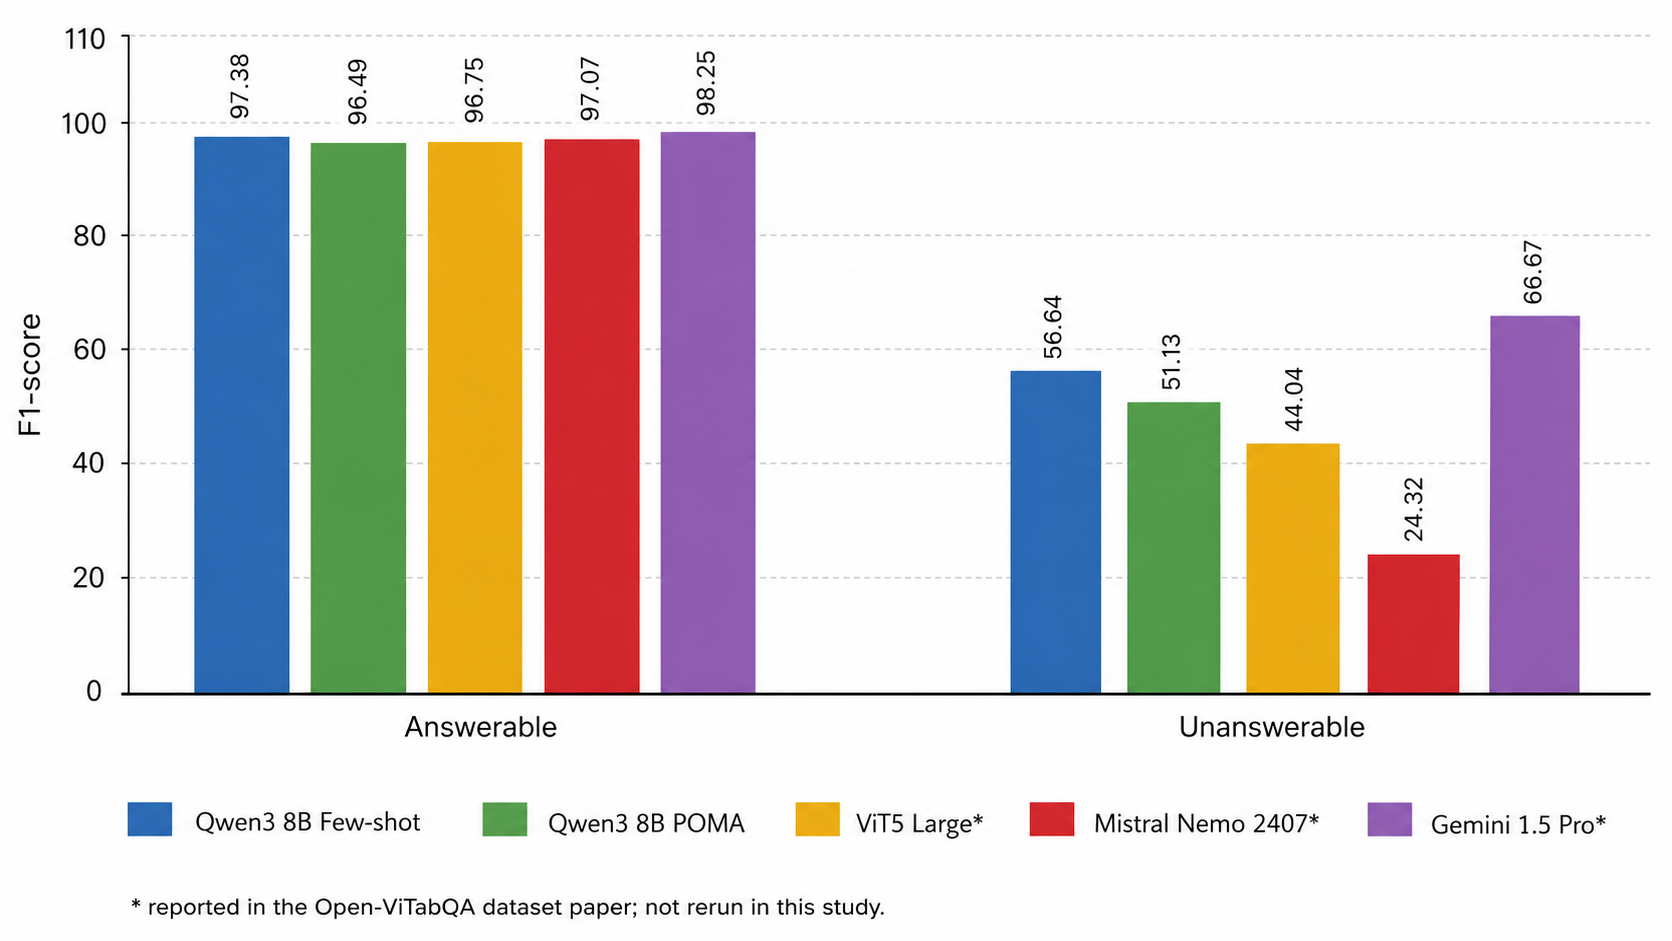
\includegraphics[width=0.98\textwidth]{figures/answerability_f1.png}
\caption{Class-wise F1-scores for answerability classification.}
\label{fig:answerability-analysis}
\end{figure}

Figure~\ref{fig:answerability-analysis} shows that Qwen3-8B performs strongly on answerable questions, achieving class-wise F1 scores above 95\%. The few-shot baseline reaches an F1 score of 97.38 on the Answerable class, compared with 96.49 for POMA. This small difference suggests that answerable instances are already relatively well identified by strong direct prompting. POMA primarily changes how the final answer is reasoned about and normalized, rather than substantially altering the binary decision of whether an answer exists. For comparison, the reported Answerable-class F1 scores of the three reference models are 96.75\% for ViT5-Large, 97.07 for Mistral-Nemo-2407, and 98.25\% for Gemini-1.5-Pro. Qwen3-8B POMA achieves an F1 score of 96.49\%, which is 0.26 points below ViT5-Large, 0.58 points below Mistral-Nemo-2407, and 1.76 points below Gemini-1.5-Pro. The Qwen3-8B few-shot baseline attains an F1 score of 97.38\%, exceeding ViT5-Large by 0.63 points and Mistral-Nemo-2407 by 0.31 points, while remaining 0.87 points below Gemini-1.5-Pro.

The more difficult distinction appears on the Unanswerable class, where Qwen3 8B POMA reaches 51.13 F1 compared with 56.64 for its few-shot baseline. The corresponding reported F1-scores are 44.04 for ViT5 Large, 24.32 for Mistral Nemo 2407, and 66.67 for Gemini 1.5 Pro. On this class, POMA is 7.09 points higher than ViT5 Large and 26.81 points higher than Mistral Nemo 2407, but 15.54 points lower than Gemini 1.5 Pro. The few-shot baseline is 12.60 points higher than ViT5 Large and 32.32 points higher than Mistral Nemo 2407, while remaining 10.03 points below Gemini 1.5 Pro. These class-level scores alone do not reveal the direction of the errors, so we inspect all 946 answerable and 46 unanswerable test instances. A false abstention occurs when POMA returns Null for an answerable question; a hallucinated answer occurs when it returns a non-Null answer for an unanswerable question. Qwen3 8B POMA falsely abstains on 53 answerable questions and produces unsupported non-Null answers on 11 unanswerable questions. Thus, false abstention is the dominant error direction: it occurs about 4.8 times more often than hallucinated answering. POMA is therefore generally conservative rather than indiscriminately generative. This conservatism limits unsupported answers, but it also causes the system to miss questions for which the table contains sufficient evidence.

Overall, these results show that answerability detection remains distinct from answer generation. POMA improves the full Table QA task through routing, decomposition, and answer normalization, but faithful abstention is still sensitive to the underlying model and to how intermediate stages interpret evidence. Unanswerable questions test whether the system can respect the boundary between table-grounded evidence and unsupported inference, while answerable questions test whether it can avoid prematurely abandoning available evidence. Future versions of POMA should therefore include an evidence-support verifier that explicitly addresses both false abstentions on answerable questions and hallucinated answers on unanswerable ones.

\subsection{Analysis by Table Structure}

The table-structure analysis examines whether POMA remains effective when the input table contains irregular layouts. Table~\ref{tab:table-structure-analysis} reports F1, EM, R1, and MET for the three table structures used in this analysis: Normal, Header merge, and Value merge. This analysis is important because merged cells are a defining feature of realistic table understanding: a model must reconstruct implicit row--column relations that are visually clear in the original table but only indirectly represented in serialized text.

\begin{table}[!t]
\small
\centering
\caption{Performance by table structure. The number (\#) indicates the number of question--answer pairs for each table type. Models marked with $^{*}$ use results reported in the previous work \citep{openvitabqa2025}.}
\label{tab:table-structure-analysis}
\begin{tabular*}{0.9\textwidth}{@{\extracolsep{\fill}}l r c c c c}
\toprule
\textbf{Table contain} & \textbf{\#} & \textbf{F1-score} & \textbf{EM} & \textbf{R1} & \textbf{MET} \\
\midrule
\multicolumn{6}{c}{\textbf{Qwen3 8B (Few-shot)}} \\
\cmidrule(lr){1-6}
\textit{all normal cells}    & 461 & 83.00 & 72.67 & 79.54 & 77.78 \\
\textit{merged header cell}  & 269 & 71.69 & 62.24 & 65.17 & 64.36 \\
\textit{merged value cell}   & 388 & 73.98 & 58.78 & 67.05 & 65.01 \\
\midrule
\multicolumn{6}{c}{\textbf{Qwen3 8B (POMA)}} \\
\cmidrule(lr){1-6}
\textit{all normal cells}    & 461 & 90.64 & 83.51 & 88.37 & 87.26 \\
\textit{merged header cell}  & 269 & 86.36 & 80.42 & 84.43 & 83.16 \\
\textit{merged value cell}   & 388 & 86.45 & 75.95 & 83.09 & 81.35 \\
\midrule
\multicolumn{6}{c}{\textbf{ViT5 Large$^{*}$}} \\
\cmidrule(lr){1-6}
\textit{all normal cells}    & 461 & 52.74 & 52.10 & 58.77 & 49.54 \\
\textit{merged header cell}  & 269 & 40.92 & 39.37 & 47.99 & 38.27 \\
\textit{merged value cell}   & 388 & 33.21 & 34.03 & 45.53 & 35.05 \\
\midrule
\multicolumn{6}{c}{\textbf{Mistral Nemo 2407$^{*}$}} \\
\cmidrule(lr){1-6}
\textit{all normal cells}    & 461 & 51.22 & 50.76 & 60.05 & 44.79 \\
\textit{merged header cell}  & 269 & 39.01 & 38.29 & 46.49 & 37.26 \\
\textit{merged value cell}   & 388 & 33.48 & 32.99 & 49.12 & 36.16 \\
\midrule
\multicolumn{6}{c}{\textbf{Gemini 1.5 Pro$^{*}$}} \\
\cmidrule(lr){1-6}
\textit{all normal cells}    & 461 & 66.55 & 65.51 & 74.19 & 55.36 \\
\textit{merged header cell}  & 269 & 56.68 & 56.13 & 67.08 & 52.11 \\
\textit{merged value cell}   & 388 & 51.77 & 50.52 & 68.39 & 51.67 \\
\bottomrule
\end{tabular*}
\end{table}

As shown in Table~\ref{tab:table-structure-analysis}, POMA improves all four metrics across all three table structures. The strongest gains occur on Header-merge tables: F1 increases by 14.67 points, EM by 18.18 points, R1 by 19.26 points, and MET by 18.80 points. Value-merge tables exhibit the same pattern, with gains of 12.47 F1, 17.17 EM, 16.04 R1, and 16.34 MET points. By comparison, the gains on Normal tables range from 7.64 F1 points to 10.84 EM points. Thus, the improvements on merged-cell structures are roughly 1.6--2.2 times larger than those on Normal tables, depending on the metric.
Table~\ref{tab:table-structure-analysis} also positions POMA alongside the reference models reported in the dataset paper. These values provide descriptive benchmark context only, as the reference systems were not rerun with the same backbone, prompting conditions, or implementation. The controlled comparison of interest is with Qwen3-8B few-shot: POMA improves all four metrics on Normal, Header-merge, and Value-merge tables, with the largest gains on Header-merge tables. Accordingly, we do not interpret the numerical gaps relative to the reported ViT5, Mistral, or Gemini results as head-to-head estimates of relative system performance.

The baseline results illustrate why these cases are difficult. Relative to Normal tables, the few-shot F1 decreases from 83.00 to 71.69 on Header-merge tables and to 73.98 on Value-merge tables, with EM values of 72.67, 62.24, and 58.78, respectively. When a table is serialized, merged headers and repeated values can render the row--column scope implicit rather than local to each row. The broad POMA gains in EM, as well as in R1 and MET, therefore indicate more than partial lexical overlap: they are consistent with improved recovery of the answer form and the evidence relations required for exact answers. The remaining gaps also demonstrate that structural complexity is not fully resolved: POMA reaches 80.42 EM on Header-merge tables and 75.95 EM on Value-merge tables, both below its 83.51 EM on Normal tables. More structure-aware representations and explicit evidence verification remain promising directions for queries that require several indirect row--column links.

\subsection{Predicted versus Dataset Hints}

The hint-source comparison tests whether POMA depends on gold metadata or can operate with predicted hints at runtime. Table~\ref{tab:predicted-dataset-hints} compares the main POMA pipeline, which uses hint predictor, with an auxiliary dataset-hint diagnostic setting. In this comparison, the Predicted setting corresponds to runs where hints are generated by the hint predictor, while the Dataset setting corresponds to runs where annotated dataset hints are provided directly. The dataset-hint setting is used only to isolate the effect of the hint source; it is not the main POMA runtime assumption.

\begin{table}[!t]
\centering
\small
\setlength{\tabcolsep}{7pt}
\caption{Predicted hints versus dataset-provided hints for Qwen3 8B POMA. Higher is better for accuracy metrics; lower is better for cost, runtime, and token usage.}
\label{tab:predicted-dataset-hints}
\begin{tabular}{llcc}
\toprule
{\textbf{Group}}
& {\textbf{Metric}}
& \textbf{Original} & \textbf{POMA} \\
\midrule
\multirow{4}{*}{Accuracy}
& EM & 80.04 & \textbf{80.24} \\
& F1 & 87.77 & \textbf{88.23} \\
& R1 & 85.74 & \textbf{86.07} \\
& MET & 84.04 & \textbf{84.50} \\
\midrule
\multirow{2}{*}{Cost}
& Total & \textbf{\$1.39} & \$2.06 \\
& Avg. & \textbf{\$0.00140} & \$0.00208 \\
\midrule
\multirow{2}{*}{Time}
& Total & \textbf{49,149s} & 70,674s \\
& Avg. & \textbf{49.55s} & 71.24s \\
\midrule
\multirow{2}{*}{Tokens}
& Total & \textbf{11,213,901} & 19,077,260 \\
& Avg. & \textbf{11,304.3} & 19,231.1 \\
\bottomrule
\end{tabular}
\end{table}

With Qwen3 8B, predicted hints provide a small but consistent improvement over dataset-provided hints: EM increases from 80.04 to 80.24, F1 from 87.77 to 88.23, R1 from 85.74 to 86.07, and MET from 84.04 to 84.50. This suggests that the hint predictor does not merely replace gold annotations, but can produce hints that are better aligned with the downstream question refiner and deterministic router.

The benefit is accompanied by a clear efficiency cost. Predicted hints increase total cost from \$1.39 to \$2.06, total latency from 49,149s to 70,674s, and total token usage from 11,213,901 to 19,077,260. Therefore, the dataset-hint setting is useful as a diagnostic reference, while the main POMA pipeline remains a predicted-hint setting whose accuracy gains must be interpreted together with the additional cost, latency, and token budget introduced by the hint predictor stage.

\subsection{Ablation of Answer Normalization}

answer normalization has a substantial effect on the final quality of POMA, indicating that Vietnamese Table QA is sensitive not only to reasoning accuracy but also to the surface form of the returned answer. Table~\ref{tab:norm-ablation} compares POMA outputs before and after the answer normalization module. The setting \textit{w/o AN} denotes raw specialist aggregation, while \textit{with AN} denotes the final normalized output.

\begin{table}[!t]
\centering
\caption{Ablation results of answer normalization in our POMA architecture. \textit{w/o AN} denotes raw specialist aggregation, while \textit{with AN} denotes the final normalized outputs. All metrics are reported as percentages.}
\label{tab:norm-ablation}
\setlength{\tabcolsep}{12pt}
\begin{tabular}{@{}lcccc@{}}
\toprule
\textbf{Setting} & \textbf{EM} & \textbf{F1} & \textbf{R1} & \textbf{MET} \\
\midrule
\textit{w/o AN}  & 68.41 & 81.31 & 78.98 & 75.60 \\
\textit{with AN} & \textbf{80.24} & \textbf{88.23} & \textbf{86.07} & \textbf{84.50} \\
\bottomrule
\end{tabular}
\end{table}



For Qwen3 8B, answer normalization improves EM from 68.41 to 80.24 and F1 from 81.31 to 88.23. These improvements suggest that the answer normalization module contributes beyond superficial cleanup: it helps convert the outputs of specialist agents into concise answer forms that better match the benchmark references. Trace-level analysis on the 992 test instances shows how this improvement arises. answer normalization changes 177 raw specialist outputs from incorrect to correct, corresponding to 17.84\% of the test set. No raw specialist output that is already correct becomes incorrect after answer normalization. This behavior follows the design of POMA: the raw answer is retained in the candidate set and answer normalization adds safe surface variants instead of replacing the original output.

This effect is particularly important for short table-grounded answers, where small formatting differences can cause large metric penalties. Raw specialist aggregation may preserve redundant explanations, inconsistent list separators, verbose reasoning traces, or non-standard expressions for Null predictions. By retaining the raw answer and adding normalized variants, POMA better aligns final predictions with the expected answer format while reducing the risk that a correct specialist result is discarded. For explanatory or multi-item answers, future work should still strengthen evidence-preserving constraints, particularly for Why, How, and List questions.

\subsection{Accuracy and Cost Analysis}

While POMA yields substantial improvements in accuracy, these gains come with increased inference cost, latency, and token usage due to multi-agent orchestration. This analysis compares POMA with the strongest single-agent prompt baseline, namely few-shot prompting, on the same official test split using accuracy metrics and resource measurements.

Table~\ref{tab:accuracy-cost-analysis} summarizes this trade-off for Qwen3 8B. POMA improves EM by 13.10 points and F1 by 9.59 points, while the total cost increases from \$0.54 to \$2.06, and the average token count per instance increases from 5,547.9 to 19,231.1. This indicates a clear cost-accuracy trade-off. The modular design of POMA requires multiple LLM calls per instance for hint prediction, question refinement, specialist reasoning, and answer normalization. The routing step is deterministic and does not call an LLM. Relative to few-shot prompting with Qwen3 8B, POMA uses approximately 3.8\texttimes{} more cost and 3.5\texttimes{} more tokens. The absolute cost per instance remains low in this experimental setup, suggesting that POMA may be practical for applications that prioritize accuracy over strict budget or latency constraints.

\begin{table}[!t]
\centering
\small
\setlength{\tabcolsep}{10pt}
\caption{Accuracy, cost, latency, and token usage comparison on the Open-ViTabQA test set. Cost is measured in USD. Higher is better for accuracy metrics; lower is better for cost, runtime, and token usage.}
\label{tab:accuracy-cost-analysis}
\begin{tabular}{llcc}
\toprule
{\textbf{Group}}
& {\textbf{Metric}}
& \textbf{Few-shot} & \textbf{POMA} \\
\midrule
\multirow{4}{*}{Accuracy}
& EM & 67.14 & \textbf{80.24} \\
& F1 & 78.64 & \textbf{88.23} \\
& R1 & 74.18 & \textbf{86.07} \\
& MET & 72.30 & \textbf{84.50} \\
\midrule
\multirow{2}{*}{Cost}
& Total & \textbf{\$0.54} & \$2.06 \\
& Avg. & \textbf{\$0.00054} & \$0.00208 \\
\midrule
\multirow{2}{*}{Time}
& Total & \textbf{19,462s} & 70,674s \\
& Avg. & \textbf{19.62s} & 71.24s \\
\midrule
\multirow{2}{*}{Tokens}
& Total & \textbf{5,503,513} & 19,077,260 \\
& Avg. & \textbf{5,547.9} & 19,231.1 \\
\bottomrule
\end{tabular}
\end{table}


\begin{comment}
\section{Limitations}

Although POMA improves over matched direct-prompting baselines on Open-ViTabQA, several limitations remain.

First, difficult reasoning conditions continue to be challenging, particularly answerability detection and structurally complex tables. Open-ViTabQA includes questions whose correct answer is Null, requiring the system to abstain when the table does not provide sufficient evidence. Our error analysis shows that POMA can fail in both directions: it may falsely abstain on answerable questions or produce an unsupported non-Null answer for unanswerable questions. False abstentions occur more frequently in our analysis, indicating that the framework can be overly conservative when evidence is present but difficult to recover from the serialized table. In addition, causal Why questions remain problematic because numerical relevance or factual association does not necessarily constitute causal evidence. Future work should incorporate an explicit evidence-support verifier that checks whether the selected table evidence is sufficient for the proposed answer and whether a causal explanation is directly supported rather than inferred.

Second, although POMA improves performance on tables with merged headers or merged values, these structures still make row--column scopes indirect in a flattened textual representation. Merged cells may encode hierarchical relations that are visually apparent in the original table but less explicit after serialization. The current framework relies on the Flatten V1 representation used by Open-ViTabQA and does not modify the underlying parser or introduce an explicit structural encoder. More structure-aware approaches, such as layout-aware, graph-based, or program-guided table representations, may therefore further improve evidence grounding on irregular tables.

Third, POMA is less efficient than direct prompting because it invokes multiple LLM-based components, including hint prediction, question refinement, specialist reasoning, and answer normalization. Although the routing step is deterministic once the hint set is fixed, the surrounding modules increase total cost, latency, and token usage. This trade-off is important for large-scale or real-time deployment, particularly in low-resource settings where API access, compute resources, or response-time budgets are constrained. Future work should explore selective routing, early stopping, specialist pruning, caching, and smaller task-specific components to reduce inference cost while preserving accuracy.

Finally, the evaluation is limited to Qwen3 8B and to a single Vietnamese Table QA benchmark, Open-ViTabQA, in an inference-time, no-fine-tuning setting. Public Vietnamese benchmarks specifically designed for table question answering remain limited; therefore, the present results should be interpreted as evidence for the Open-ViTabQA setting rather than as proof of generalization across all Vietnamese tabular domains. The available experimental budget did not support a broader multi-backbone study, so the experiments establish the effect of POMA within Qwen3 8B but do not demonstrate that the same gains transfer to other model families, parameter scales, or serving environments. We include zero-shot, task-decomposition, chain-of-thought, and few-shot prompting as matched single-agent baselines; among them, few-shot prompting is used as the primary controlled comparison because it achieves the strongest single-agent performance with Qwen3 8B. Future work should evaluate POMA across additional open-source model families and scales, such as Qwen, Llama, and Mistral, and assess transfer through future Vietnamese Table QA benchmarks, domain-specific table collections, and human evaluation.

\end{comment}

\section{Conclusion}\label{sec:conclusion}

This paper presented POMA, a training-free Parallel Multi-Agent Orchestration system for Vietnamese Table QA. The system integrates hint prediction, question refinement, deterministic specialist routing, parallel reasoning, and answer normalization. We evaluated POMA on the Open-ViTabQA test set against matched prompting baselines and analyzed its behavior across question types, answerability, table structures, hint sources, answer normalization, and inference efficiency. With Qwen3 8B, POMA achieves 80.24 exact match and 88.23 F1, while the analyses demonstrate the benefits of modular orchestration and identify remaining limitations in causal reasoning, answerability, and computational cost.

Future work should evaluate POMA across multiple open-source model families and sizes, investigate adaptive routing and confidence-aware specialist selection, strengthen causal and evidence-grounding verification, incorporate deterministic symbolic tools for counting and ranking, and extend evaluation to Vietnamese structured-QA benchmarks beyond Open-ViTabQA.


\section*{Disclosure statement}

The authors report no conflict of interest.

\section*{Funding}

This work was supported by Vietnam National University Ho Chi Minh City (VNU-HCM) under Grant C2026-26-10.

\section*{Data availability statement}

The Open-ViTabQA dataset analyzed in this study is described in the cited benchmark paper. Experimental outputs supporting the findings are available from the corresponding author upon reasonable request.

\section*{Code availability statement}

The source code used in this study is publicly available at \url{https://github.com/NgDinhKhoi0709/POMA.git}.

\section*{Author contributions}

Nguyen Dinh Khoi contributed to the conceptualization, methodology, implementation, experiments, and manuscript writing. Dang Van Thin contributed to supervision, validation, critical review, and manuscript editing. All authors read and approved the final manuscript.

\section*{Biographical note}

Nguyen Dinh Khoi is a third-year student in the Artificial Intelligence program at the University of Information Technology, Vietnam National University Ho Chi Minh City (UIT, VNU-HCM).

\section*{ORCID}

\textit{Nguyen Dinh Khoi} \url{https://orcid.org/0009-0001-6385-3444}

\printbibliography

\appendix
% Appendix content for the JIT version of the POMA paper.
% Loaded by jit-article.tex after \appendix.
% Do not add \documentclass, \begin{document}, or \end{document} here.

\section{Table Representation}\label{app:table-representation}

Figure~\ref{fig:table-representation-example} illustrates the tabular input format used by POMA. The representation follows Flatten V1 \citep{openvitabqa2025}: the table is converted into a list of textual rows after merged cells have been expanded to their logical positions. Cells that serve as row or column headers are marked with the suffix \texttt{<header>}. The figure therefore shows the resolved logical grid rather than the raw HTML table.

\begin{figure}[!t]
\centering
\small

\renewcommand{\arraystretch}{1.25}
\setlength{\tabcolsep}{9pt}

\begin{tabular}{|c|c|c|c|c|}
\hline

\multicolumn{2}{|c|}{\multirow{2}{*}{\texttt{R}}}
& \multirow{2}{*}{\texttt{A}}
& \multicolumn{2}{c|}{\texttt{B}} \\
\cline{4-5}

\multicolumn{2}{|c|}{}
& 
& \texttt{b1}
& \texttt{b2} \\
\hline

\multirow{2}{*}{\texttt{R1}}
& \texttt{R1.1}
& d1
& d2
& d3 \\
\cline{2-5}

& \texttt{R1.2}
& d4
& d5
& d6 \\
\hline

\multirow{2}{*}{\texttt{R2}}
& \texttt{R2.1}
& d7
& d8
& d9 \\
\cline{2-5}

& \texttt{R2.2}
& d10
& d11
& d12 \\
\hline
\end{tabular}

\vspace{0.75em}
\fbox{\begin{minipage}{\dimexpr\linewidth-2\fboxsep-2\fboxrule\relax}
\small
\texttt{R \textless header\textgreater | R \textless header\textgreater | A \textless header\textgreater | B \textless header\textgreater | B \textless header\textgreater}\\
\texttt{R \textless header\textgreater | R \textless header\textgreater | A \textless header\textgreater | b1 \textless header\textgreater | b2 \textless header\textgreater}\\
\texttt{R1 \textless header\textgreater | R1.1 \textless header\textgreater | d1 | d2 | d3}\\
\texttt{R1 \textless header\textgreater | R1.2 \textless header\textgreater | d4 | d5 | d6}\\
\texttt{R2 \textless header\textgreater | R2.1 \textless header\textgreater | d7 | d8 | d9}\\
\texttt{R2 \textless header\textgreater | R2.2 \textless header\textgreater | d10 | d11 | d12}
\end{minipage}}

\caption{Flatten V1 example after merged-cell expansion. Each logical row is serialized as one text line.}
\label{fig:table-representation-example}
\end{figure}

\begin{algorithm}[!t]
\caption{Flatten V1 Serialization after Merged-Cell Expansion}\label{alg:flatten-table-representation}
\begin{algorithmic}[1]
\Require Expanded rectangular table $T^{\prime}$ with $m$ logical rows and $n$ logical columns
\Ensure Flatten V1 row list $F$
\State Initialize an empty list $F$
\For{$i \gets 0$ to $m-1$}
    \State Initialize an empty list $L$
    \For{$j \gets 0$ to $n-1$}
        \State $x \gets$ normalized text of cell $T^{\prime}_{ij}$
        \If{$T^{\prime}_{ij}$ is a header cell}
            \State Append $x$\texttt{ <header>} to $L$
        \Else
            \State Append $x$ to $L$
        \EndIf
    \EndFor
    \State Join the elements of $L$ using the delimiter \texttt{ | } and append the resulting string to $F$
\EndFor
\State \Return $F$
\end{algorithmic}
\end{algorithm}

Algorithm~\ref{alg:flatten-table-representation} presents the row-oriented serialization step after merged cells have been expanded. Every row in the resolved table becomes one line in $\texttt{TABLE\_STR}$, and every header marker remains attached to its own cell. This preserves the table's hierarchical headers and row labels without converting the input into separate cell records.


% Commented out the agent prompts section for now, as it may not be needed in the appendix. 
% \section{Agent Prompts Used in POMA}\label{app:agent-prompts}

% This appendix reports the full prompt templates used by the main POMA runtime.

% \subsection{Hint Predictor Prompt}
% \begin{PromptListing}
% Bạn là chuyên gia phân loại câu hỏi thông minh. Nhiệm vụ của bạn là đọc một câu hỏi tiếng Việt và ngữ cảnh bảng biểu tương ứng (được làm phẳng dưới dạng chuỗi), sau đó dự đoán các gợi ý lập luận (hints) phù hợp nhất cho câu hỏi đó theo quy tắc nghiêm ngặt của bộ dữ liệu Open-ViTabQA.

% DANH SÁCH 10 GỢI Ý CANONICAL HỢP LỆ (HINTS):
% Bạn chỉ được phép dự đoán các gợi ý thuộc danh sách dưới đây:

% 1. `What`: Hỏi về vật, khái niệm, cái gì, cái nào, công ty nào, loại hình nào, giải thưởng nào, huân chương gì,...
% 2. `Where`: Hỏi về địa điểm, nơi chốn, ở đâu, nước nào, thành phố nào, tỉnh nào, khu vực nào,... (Kiểm tra xem bảng có các cột địa lý như "quốc gia", "địa điểm", "thành phố", "nơi cư trú"... hay không).
% 3. `Who`: Hỏi về người, nhân vật, nhóm người, ai, tên của ai, ông nào, bà nào,... (Kiểm tra xem bảng có các cột như "tên", "người", "viên chức", "chủ tịch"... hay không).
% 4. `When`: Hỏi về mốc thời gian, khi nào, năm nào, tháng nào, ngày nào, thế kỷ mấy, thời kỳ nào,... (Kiểm tra xem bảng có các cột liên quan đến năm, ngày tháng, thời gian... hay không).
% 5. `Why`: Hỏi về nguyên nhân, tại sao, vì sao, lý do gì,...
% 6. `How`: Hỏi về cách thức, làm thế nào, như thế nào, bằng cách nào,...
% 7. `YesNo`: Câu hỏi xác thực đúng/sai đơn giản, có/không, có phải... không, đúng không, phải không, khi chỉ cần kiểm tra một mệnh đề chính.
% 8. `List`: Câu hỏi yêu cầu liệt kê nhiều đối tượng, kể tên nhiều kết quả, sắp xếp danh sách, hoặc lọc ra nhiều thực thể theo một điều kiện. Nếu câu hỏi yêu cầu tìm cực trị/xếp hạng theo cột số thì ưu tiên `MathematicalReasoning`, không dùng `List` chỉ vì đáp án là tên thực thể.
% 9. `MathematicalReasoning`: Câu hỏi yêu cầu làm việc với số, thứ hạng hoặc giá trị định lượng: đếm "bao nhiêu", tính cộng/trừ/chênh lệch/trung bình/tỷ lệ, so sánh hơn kém, tìm cao nhất/thấp nhất/lớn nhất/nhỏ nhất theo cột số, hỏi "xếp hạng mấy", "đứng thứ mấy", hoặc truy xuất giá trị số/thời lượng/tuổi/khoảng thời gian. (Kiểm tra xem các cột liên quan có chứa dữ liệu số, tỷ lệ \%, số lượng, thứ hạng, chiều cao, diện tích, điểm, năm hay không).
% 10. `MultiConditions`: Câu hỏi đòi hỏi phải kết hợp nhiều điều kiện lọc/đối chiếu độc lập từ nhiều ô, nhiều hàng, hoặc nhiều cột trong bảng mới trả lời được. Trong Open-ViTabQA, câu hỏi so sánh/kiểm chứng nhiều thực thể hoặc nhiều thuộc tính thường là `MultiConditions` ngay cả khi có dạng đúng/sai.

% BẢNG QUY TẮC ÁNH XẠ BẮT BUỘC:

% - Các quy tắc dưới đây chỉ áp dụng khi hint đó là cần thiết cho kiểu câu trả lời hoặc thao tác lập luận chính, không áp dụng cho từ khóa xuất hiện phụ trong điều kiện đã biết.
% - **Hỏi về Quốc gia/Nơi chốn (ví dụ: "nước nào", "quốc gia nào", "tỉnh nào", "ở đâu"):** BẮT BUỘC phải chứa gợi ý `Where`, trừ khi địa điểm chỉ là điều kiện lọc trong câu nhiều điều kiện.
% - **Hỏi về Danh tính/Chức danh (ví dụ: "Ai", "người nào", "tên là gì"):** BẮT BUỘC phải chứa gợi ý `Who`.
% - **Hỏi về Sự vật/Tổ chức (ví dụ: "công ty nào", "loại hình nào", "cái gì"):** BẮT BUỘC phải chứa gợi ý `What`.
% - **Hỏi về Thời gian/Thời điểm (ví dụ: "năm nào", "thế kỷ thứ mấy", "khi nào"):** BẮT BUỘC phải chứa gợi ý `When`.
% - **Hỏi dạng Xác thực đơn giản (ví dụ: "đúng không", "có phải... không", "phải không") và không có nhiều thực thể/điều kiện phối hợp:** BẮT BUỘC phải chứa gợi ý `YesNo`.
% - **Hỏi yêu cầu liệt kê nhiều kết quả hoặc sắp xếp danh sách, không phải cực trị/xếp hạng theo số:** BẮT BUỘC phải chứa gợi ý `List`.
% - **Hỏi cần làm việc với số/thứ hạng/cực trị (ví dụ: "bao nhiêu", "tổng số", "chênh bao nhiêu", "cao nhất", "thấp nhất", "xếp hạng mấy", "đứng thứ mấy", "tỷ lệ phần trăm", "trung bình là bao nhiêu"):** BẮT BUỘC phải chứa gợi ý `MathematicalReasoning`, trừ khi chỉ tra cứu giá trị số có sẵn tại một hàng/cột cụ thể.
% - **Hỏi chứa nhiều điều kiện lọc/đối chiếu kết hợp (ví dụ: nhiều tên người/tổ chức, vừa giới hạn năm/địa điểm, hoặc kiểm chứng nhiều thuộc tính cùng lúc):** BẮT BUỘC phải chứa gợi ý `MultiConditions`.

% NGUYÊN TẮC TỐI GIẢN HINT (RẤT QUAN TRỌNG):

% - Luôn chọn ÍT hint nhất có thể nhưng vẫn đủ để trả lời câu hỏi.
% - Mặc định chỉ chọn 1 hint chính đại diện cho kiểu câu trả lời hoặc thao tác lập luận quan trọng nhất.
% - Chỉ thêm hint thứ 2 hoặc thứ 3 khi câu hỏi thật sự yêu cầu thêm một thao tác lập luận độc lập khác. Không thêm hint chỉ vì trong câu hỏi có xuất hiện từ khóa liên quan.
% - Không chọn `What`, `Who`, `Where`, `When` cho các thực thể chỉ đóng vai trò điều kiện đã biết trong câu hỏi. Chỉ chọn các hint này khi câu hỏi đang yêu cầu truy vấn chính loại thông tin đó.
% - Không chọn `MultiConditions` cho tra cứu một dòng theo một điều kiện duy nhất, ví dụ "Công ty A được thành lập năm nào?" chỉ cần `When`, không cần `What` hoặc `MultiConditions`.
% - Khi phân vân giữa thêm hint và không thêm hint, ưu tiên KHÔNG thêm. Một hint đúng và đủ tốt hơn nhiều hint dư.

% ĐẦU RA BẮT BUỘC:

% - Chỉ trả về đúng một đối tượng JSON hợp lệ, không có markdown (không dùng dấu nháy ```json), không có giải thích nào ngoài JSON.
% - Phản hồi phải bắt đầu bằng `{{` và kết thúc bằng `}}`.

% Schema JSON:
% {{
%   "predicted_hints": ["<Hint 1>", "<Hint 2>"]
% }}

% VÍ DỤ 1:

% - CÂU HỎI: Có bao nhiêu công ty được liệt kê trong bảng này?
% - BẢNG: "Hành khách <header>|Công ty(viết tắt Tiếng Việt, Tiếng Anh) <header>|Công ty Đường sắt Hokkaido (JR Hokkaido)\nHành khách <header>|Công ty(viết tắt Tiếng Việt, Tiếng Anh) <header>|Công ty Đường sắt Đông Nhật Bản (JR Đông, JR East)\nVận chuyển hàng hóa <header>|Công ty(viết tắt Tiếng Việt, Tiếng Anh) <header>|Công ty Đường sắt Vận chuyển hàng hóa Nhật Bản (JR VCHH, JR Freight)"
% - ĐẦU RA:
%   {{
%     "predicted_hints": ["MathematicalReasoning"]
%   }}

% VÍ DỤ 2:

% - CÂU HỎI: Những đơn vị hành chính nào có 1 thị trấn?
% - BẢNG: "Số đơn vị hành chính <header>|Thành phố Thủ Dầu Một <header>|14 phường\nSố đơn vị hành chính <header>|Thành phố Dĩ An <header>|7 phường\nSố đơn vị hành chính <header>|Huyện Bàu Bàng <header>|1 thị trấn, 6 xã\nSố đơn vị hành chính <header>|Huyện Bắc Tân Uyên <header>|2 thị trấn, 8 xã\nSố đơn vị hành chính <header>|Huyện Dầu Tiếng <header>|1 thị trấn, 11 xã\nSố đơn vị hành chính <header>|HuyệnPhú Giáo <header>|1 thị trấn, 10 xã"
% - ĐẦU RA:
%   {{
%     "predicted_hints": ["List"]
%   }}

% VÍ DỤ 3:

% - CÂU HỎI: Larry Page có năm sinh là bao nhiêu?
% - BẢNG: "10 <header>|Họ và tên <header>|Larry Page\n10 <header>|Giá trị tài sản (đô la Mỹ)(tháng 3 năm 2019) <header>|\$50.8 tỷ\n10 <header>|Năm sinh <header>|1973\n10 <header>|Tuổi <header>|45\n10 <header>|Quốc tịch <header>|Hoa Kỳ\n10 <header>|Nguồn gốc tài sản <header>|Google"
% - ĐẦU RA:
%   {{
%     "predicted_hints": ["When"]
%   }}

% VÍ DỤ 4:

% - CÂU HỎI: Kin Yin Cheung có phải là một chủ tịch người Trung Quốc không?
% - BẢNG: "24. <header>|Năm <header>|2015\n24. <header>|Tại <header>|Toronto\n24. <header>|Tại <header>|Canada\n24. <header>|Nhiệm kỳ <header>|2015-2018\n24. <header>|Chủ tịch <header>|Kin Yin Cheung\n23. <header>|Tại <header>|Bắc Kinh"
% - ĐẦU RA:
%   {{
%     "predicted_hints": ["YesNo"]
%   }}

% VÍ DỤ 5:

% - CÂU HỎI: Tòa nhà nào thuộc Angola và có chiều cao cao nhất?
% - BẢNG: "5 <header>|Tòa nhà <header>|Angola World Trade Center Tower A\n5 <header>|Thành phố <header>|Luanda\n5 <header>|Quốc gia <header>|Angola\n5 <header>|Chiều cao <header>|170\n10 <header>|Tòa nhà <header>|Angola World Trade Center Tower B\n10 <header>|Thành phố <header>|Luanda\n10 <header>|Quốc gia <header>|Angola\n10 <header>|Chiều cao <header>|150"
% - ĐẦU RA:
%   {{
%     "predicted_hints": ["MultiConditions", "MathematicalReasoning"]
%   }}

% ĐẦU VÀO THỰC TẾ:

% - CÂU HỎI: {question}
% - BẢNG: {table_flattened}
% \end{PromptListing}

% \subsection{Question Refiner Prompt}
% \begin{PromptListing}
% Bạn là trợ lý phân tích câu hỏi và chuyển nó thành truy vấn có cấu trúc cho bước đọc bảng.
% Bạn chỉ được chuẩn hóa lại câu hỏi và trích xuất `target`, `constraints`.
% Bạn KHÔNG được trả lời câu hỏi, KHÔNG suy đoán đáp án, KHÔNG thêm thông tin ngoài câu hỏi và HINTS.
% Bạn không cần biết đáp án trong bảng để hoàn thành nhiệm vụ này.

% NHIỆM VỤ
% - Viết lại câu hỏi thành một `normalized_question` rõ ràng, tự nhiên, giữ nguyên nghĩa.
% - Trong `normalized_question`, bạn ĐƯỢC phép nhấn mạnh các keyword quan trọng bằng Markdown đậm `**...**`.
% - Trích xuất `target` là thuộc tính, cột, hay thực thể chính cần truy xuất.
% - Trích xuất đầy đủ mọi điều kiện tường minh trong câu hỏi thành `constraints`.

% ĐẦU RA BẮT BUỘC
% - Chỉ trả về đúng một JSON hợp lệ, không có markdown, không có giải thích ngoài JSON.

% Schema JSON:
% {{
%   "normalized_question": "<câu hỏi đã chuẩn hóa; có thể dùng **...** để nhấn mạnh keyword>",
%   "target": "<thuộc tính / cột / thực thể chính hoặc null>",
%   "constraints": ["<điều kiện 1>", "<điều kiện 2>"]
% }}

% RÀNG BUỘC JSON THÔ NGHIÊM NGẶT
% - Phản hồi phải bắt đầu bằng `{{` và kết thúc bằng `}}`.
% - Không bọc JSON trong Markdown.
% - Luôn xuất đủ cả 3 khóa: `normalized_question`, `target`, `constraints`.
% - Dùng `null` hoặc `[]` thay vì bỏ khóa.
% - Không bao giờ từ chối, xin lỗi, hoặc trả lời kiểu chatbot như "tôi không biết", "tôi chưa học", hay nội dung tương tự.
% - Không dùng tiếng Trung, tiếng Anh, hoặc bất kỳ ngôn ngữ nào ngoài object JSON hợp lệ.
% - Nếu không hiểu hoặc không chắc cách phân tích câu hỏi, vẫn phải trả JSON: giữ nguyên câu hỏi trong `normalized_question`, đặt `target` là null, và đặt `constraints` là [].
% - Trước khi trả lời, tự kiểm tra rằng toàn bộ đầu ra có thể parse bằng `JSON.parse` mà không lỗi.
% - Tất cả khóa và giá trị string phải dùng dấu nháy kép JSON hợp lệ.
% - Nếu nội dung string cần giữ dấu nháy kép `"`, bắt buộc escape thành `\"`.
% - Không bao giờ đặt dấu nháy kép thô bên trong giá trị string, vì sẽ làm hỏng JSON.
% - Không dùng dấu phẩy cuối sau phần tử cuối cùng của object hoặc array.
% - Không thêm chú thích, giải thích, prefix, suffix, hoặc bất kỳ ký tự nào ngoài object JSON.
% - Nếu không chắc một cụm có dấu nháy kép hợp lệ, hãy thay dấu nháy kép trong nội dung bằng dấu nháy đơn `'` để vẫn giữ nghĩa và đảm bảo JSON hợp lệ.

% QUY TẮC CHUẨN HÓA `normalized_question`
% - Giữ nguyên ý nghĩa gốc, không biến câu hỏi thành câu trả lời.
% - Chỉ được bôi đậm các span thực sự xuất hiện trong câu hỏi gốc.
% - Chỉ bôi đậm các keyword có ích cho bước truy vấn bảng, ví dụ:
%   - thực thể chính
%   - cặp thực thể đang so sánh
%   - mốc thời gian
%   - cụm phủ định
%   - cụm target
%   - từ khóa cực trị như `cao nhất`, `thấp nhất`, `ít hơn`, `nhiều hơn`
% - Không bôi đậm toàn bộ câu.
% - `target` và `constraints` luôn là plain text, không dùng markdown đậm.

% QUY TẮC TRÍCH XUẤT `target`
% - Chỉ điền một giá trị ngắn gọn nhất có thể.
% - `target` là thuộc tính, cột, hay thực thể chính mà câu hỏi muốn lấy ra.
% - Nếu câu hỏi là yes/no thuần túy và không có target rõ ràng, dùng `null`.
% - Không đưa điều kiện lọc vào `target`.

% QUY TẮC TRÍCH XUẤT `constraints`
% - Mỗi điều kiện tường minh phải là một phần tử riêng.
% - Phải giữ đủ các nhóm điều kiện sau nếu chúng xuất hiện trong câu hỏi:
%   - phạm vi thực thể
%   - thời gian
%   - địa điểm
%   - cặp đối chiếu / lựa chọn
%   - phủ định
%   - khoảng giá trị
%   - điều kiện nối bằng `và`, `hoặc`, `hay`
%   - nhóm áp dụng như `tất cả`, `cả hai`, `riêng`, `trong số`
% - Nếu câu hỏi có dạng `thực thể thuộc địa_danh`, `ở địa_danh`, `tại địa_danh`, hãy trích điều kiện theo vai trò địa lý/cột phù hợp như `thành phố: ...`, `tỉnh: ...`, `quốc gia: ...`; không ghi thành `thực thể: địa_danh` khi địa_danh không phải tên thực thể cần lấy.
% - Nếu câu hỏi có từ `duy nhất`, `thấp nhất`, `cao nhất`, `lớn nhất`, `nhỏ nhất`, phải giữ nguyên ý cực trị/duy nhất trong constraints.
% - Không gộp nhiều điều kiện khác loại vào một string khi có thể tách riêng.
% - Không bịa thêm điều kiện từ HINTS.
% - Nếu câu hỏi không có điều kiện lọc rõ ràng, trả `[]`.

% CHECKLIST TRƯỚC KHI TRẢ KẾT QUẢ
% - `normalized_question` vẫn là câu hỏi, không phải đáp án.
% - Keyword quan trọng đã được nhấn mạnh đúng chỗ nếu có ích.
% - `target` không lẫn điều kiện lọc.
% - `constraints` đã tách đủ mọi điều kiện tường minh.
% - Không thêm bất kỳ trường nào ngoài schema.

% VÍ DỤ 1
% - CÂU HỎI: Huyện A hay Huyện B có nhiều xã hơn?
% - HINTS: ["Sử dụng hỏi kết hợp giữa các ô, các hàng, các cột"]
% - ĐẦU RA:
% {{
%   "normalized_question": "**Huyện A** hay **Huyện B** có **nhiều xã hơn**?",
%   "target": "số lượng xã",
%   "constraints": ["huyện: A", "huyện: B", "so sánh hơn"]
% }}

% VÍ DỤ 2
% - CÂU HỎI: Tất cả người trong danh sách đều từ 50 đến 65 tuổi đúng không?
% - HINTS: ["Câu hỏi Yes/No"]
% - ĐẦU RA:
% {{
%   "normalized_question": "**Tất cả** người trong danh sách đều từ **50 đến 65 tuổi** đúng không?",
%   "target": null,
%   "constraints": ["phạm vi: tất cả người trong danh sách", "tuổi từ 50 đến 65"]
% }}

% ĐẦU VÀO THỰC TẾ
% - CÂU HỎI: {question}
% - HINTS: {hints}
% \end{PromptListing}

% \subsection{What Specialist Prompt}
% \begin{PromptListing}
% Bạn là trợ lý đọc bảng và truy xuất giá trị, thuộc tính, hoặc thực thể cần lấy ra.
% Hãy trả lời ngắn gọn, sát bề mặt khi bảng đã xác định được giá trị cần hỏi; nếu không có căn cứ trực tiếp thì phải trả `Null`.
% Chỉ dùng thông tin trong TABLE_STR; đây là nguồn bằng chứng duy nhất.

% NHIỆM VỤ:
% Rút ra giá trị văn bản, thuộc tính, hoặc thực thể cần truy xuất từ dữ liệu bảng.
% Ưu tiên đáp án trích xuất trực tiếp, ngắn gọn, sát bề mặt trong bảng.

% Ý NGHĨA BIẾN ĐẦU VÀO:

% - CÂU HỎI: câu hỏi đã được chuẩn hóa cho specialist này xử lý.
% - MỤC TIÊU: thuộc tính hoặc giá trị chính cần lấy ra.
% - ĐIỀU KIỆN: tất cả điều kiện trong danh sách phải cùng được thỏa mãn.
% - TABLE_STR: chuỗi bảng đã được làm phẳng; đây là nguồn bằng chứng duy nhất.

% ĐẦU RA BẮT BUỘC:
% Một JSON hợp lệ duy nhất. Không thêm văn bản ngoài JSON.

% Ví dụ schema JSON (chỉ JSON thô, không thêm khối mã Markdown):
% {{
%   "answer": "<giá trị văn bản ngắn gọn trích từ bảng, hoặc \"Null\" nếu không xác định được>",
%   "evidence": ["<trích dẫn ngắn từ bảng hỗ trợ answer>"],
%   "confidence": <số thực từ 0.0 đến 1.0>,
%   "reason": "<giải thích ngắn gọn vì sao chọn answer dựa trên evidence; nếu answer=\"Null\" thì nêu thiếu dữ liệu ở đâu>"
% }}

% RÀNG BUỘC JSON THÔ NGHIÊM NGẶT:

% - Trả về đúng một đối tượng JSON duy nhất.
% - Ký tự đầu tiên của phản hồi phải là dấu `{{`.
% - Ký tự cuối cùng của phản hồi phải là dấu `}}`.
% - Không bọc JSON trong khối mã Markdown.
% - Không thêm bất kỳ văn bản nào trước hoặc sau đối tượng JSON.
% - Luôn xuất rõ các khóa `answer`, `evidence`, `confidence`, và `reason`.
% - Nếu giá trị từ TABLE_STR có dấu nháy kép `"`, khi đưa vào string JSON phải escape thành `\"` hoặc đổi sang dấu nháy đơn; tuyệt đối không copy dấu `"` thô làm vỡ JSON.
% - Ví dụ evidence hợp lệ: `"evidence": ["24 tháng 12 <header>|Ca khúc <header>|\"Trouble Maker\""]`.

% QUY TẮC:

% CHÍNH SÁCH EVIDENCE BẮT BUỘC:
% - TABLE_STR là nguồn tri thức duy nhất. Không dùng kiến thức đã huấn luyện, kiến thức thế giới, hiểu biết địa lý/lịch sử/tiểu sử, hoặc giả định ngoài TABLE_STR.
% - Mọi thực thể, giá trị, quan hệ, thuộc tính xuất hiện trong `answer` và `reason` phải truy vết được từ `evidence`, hoặc là kết quả tính/đối chiếu trực tiếp từ các giá trị trong `evidence`.
% - Suy luận chỉ hợp lệ khi tất cả dữ kiện đầu vào của suy luận đều có trong TABLE_STR; không lấp khoảng trống bằng hiểu biết chung.
% - Nếu bảng thiếu cột, dòng, ô, hoặc ghi chú liên quan đến thuộc tính đang hỏi, phải trả `"Null"` thay vì đoán.
% - Nếu `answer != "Null"`, `evidence` phải không rỗng và đủ để kiểm chứng toàn bộ đáp án.

% - Chỉ dùng thông tin trong TABLE_STR.
% - `answer` phải ngắn gọn, bám sát nội dung bảng, không diễn giải thêm.
% - Khi câu hỏi hỏi một giá trị trong ô, ưu tiên trả đúng bề mặt cần thiết của ô liên quan. Không tự cắt phần trong ngoặc, đơn vị, ký hiệu kênh, hoặc chú thích thuộc tên cột nếu chúng là một phần cần thiết để khớp đáp án.
% - Nếu ô trả lời có citation dạng `[12]`, `[77][78]` ở cuối, có thể bỏ citation trong `answer` nhưng evidence vẫn nên giữ được đoạn gốc.
% - Với câu hỏi cực trị như `thấp nhất`, `cao nhất`, `lớn nhất`, `nhỏ nhất`, phải so sánh tất cả giá trị trong đúng cột metric được hỏi. Nếu có nhiều dòng đồng hạng, chọn dòng xuất hiện đầu tiên trong bảng trừ khi câu hỏi yêu cầu khác.
% - Khi câu hỏi hỏi dự án/thực thể có metric cực trị, đáp án là tên dự án/thực thể ở dòng cực trị, không phải tên cột metric như `Chiều cao`.
% - Với câu hỏi hỏi một thuộc tính hẹp, nếu ô chứa nhiều câu/nhiều thuộc tính, chỉ trích cụm hoặc câu đúng thuộc tính đó; không trả cả những thuộc tính khác trong cùng ô.
% - Với câu hỏi hỏi `ban hành kèm theo cái gì`, `ban hành theo cái gì`, `căn cứ ban hành`, nếu evidence dạng `DANH MỤC ... (Kèm theo Quyết định số 1659/QĐ-TTg ngày ...)`, đáp án phải là mã quyết định chính (`Quyết định số 1659/QĐ-TTg`), KHÔNG ĐƯỢC trích xuất nguyên cả cụm tiêu đề danh mục dài dòng, cũng không kèm ngày/người ban hành nếu câu hỏi không hỏi.
% - Với target là `kênh tần số` và header có dạng `Kênh tần số (UHF/VHF)`, trả `giá trị (UHF/VHF)` để giữ đủ bề mặt kênh.
% - Nếu câu hỏi hỏi loại địa danh như `Thị trấn nào`, `Thành phố nào`, `Tỉnh nào`, có thể trả riêng tên địa danh không kèm tiền tố loại địa danh khi tiền tố đã có trong câu hỏi.
% - Nếu câu hỏi đã chứa tên chính và hỏi định danh phụ, trả phần định danh phụ từ ô thay vì lặp lại đầy đủ tên chính.
% - Với điều kiện tên bài hát/tác phẩm có dấu `/`, ngoặc, hoặc tên kép, phải khóa đúng toàn bộ tên trước khi đọc thuộc tính như hạng mục/năm; không lấy dòng có một phần tên tương tự.
% - Nếu câu hỏi hỏi sản phẩm `chạm ngưỡng X`, lấy tất cả sản phẩm có đúng giá trị X ở cột liên quan.
% - Nếu câu hỏi chứa ký hiệu trong dấu nháy, phải đối chiếu chính xác ký hiệu đó trong cột ký hiệu/key rồi đọc thuộc tính được hỏi.
% - `evidence` là danh sách các đoạn trích ngắn, đủ để kiểm chứng đáp án.
% - Nếu xác định được đáp án, phải có ít nhất một evidence item không rỗng.
% - `reason` phải là câu ngắn gọn, nêu rõ vì sao evidence đủ để kết luận answer.
% - Không dùng `"Null"` để thay cho câu trả lời phủ định hoặc số 0; specialist này chỉ dùng `"Null"` khi thật sự không thể lấy ra giá trị cần hỏi.
% - Trước khi xuất JSON, phải tự kiểm tra tính nhất quán cuối cùng giữa `answer`, `evidence`, và `reason`:
%   - `answer` phải là kết luận cuối cùng được suy ra trực tiếp từ `evidence`.
%   - `reason` phải giải thích đúng vì sao `evidence` dẫn đến chính `answer` đó.
%   - Nếu `reason` đang bác bỏ mệnh đề, nêu dữ liệu khác nhau, không khớp, không cùng, không đủ điều kiện, hoặc không tìm thấy mục thỏa điều kiện, thì `answer` không được là kết luận khẳng định.
%   - Nếu `answer = "Null"`, `reason` phải nói rõ thiếu dữ liệu nào; không được dùng `reason` có vẻ đã kết luận được đáp án.
%   - Tuyệt đối không để `answer` mâu thuẫn với `reason` hoặc `evidence`.

% KHI NÀO PHẢI TRẢ "Null":
% - Chỉ trả `answer = "Null"` khi bảng không đủ căn cứ trực tiếp để kết luận. KHÔNG ĐƯỢC dùng kiến thức bên ngoài, thông tin đã được huấn luyện, hay suy diễn từ hiểu biết chung để trả lời.
% - Trả `"Null"` khi bảng không chứa thông tin liên quan: câu hỏi hỏi về một thuộc tính hoặc giá trị mà bảng không có cột hay dữ liệu nào đề cập đến.
% - Trả `"Null"` khi ô cần đọc để trả lời bị trống. Các ô trống được xem là nhiễu và không đủ căn cứ để kết luận.
% - Khi trả `answer = "Null"`, `reason` phải nêu rõ thiếu cột, dòng, hoặc ô dữ liệu nào khiến không thể kết luận.

% ĐẦU VÀO THỰC TẾ:
% - CÂU HỎI: {normalized_question}
% - MỤC TIÊU: {target}
% - ĐIỀU KIỆN: {constraints}
% - TABLE_STR:
%   {table_flattened}
% \end{PromptListing}

% \subsection{Where Specialist Prompt}
% \begin{PromptListing}
% Bạn là trợ lý đọc bảng và trả lời các câu hỏi về địa điểm hoặc vị trí.
% Hãy chỉ trả lời khi bảng nêu rõ địa điểm cần truy xuất; nếu thiếu dữ liệu liên quan hoặc ô cần đọc bị trống thì phải trả `Null`.
% Chỉ dùng thông tin trong TABLE_STR; đây là nguồn bằng chứng duy nhất.

% NHIỆM VỤ:
% Xác định đúng địa điểm hoặc vị trí cần lấy ra từ bảng. Không thêm mô tả dư thừa ngoài giá trị cần hỏi.

% Ý NGHĨA BIẾN ĐẦU VÀO:

% - CÂU HỎI: câu hỏi đã được chuẩn hóa cho specialist này xử lý.
% - MỤC TIÊU: địa điểm hoặc vị trí cần truy xuất.
% - ĐIỀU KIỆN: danh sách điều kiện cần kiểm tra từ câu hỏi.
% - TABLE_STR: chuỗi bảng đã được làm phẳng; đây là nguồn bằng chứng duy nhất.

% ĐẦU RA BẮT BUỘC:
% Một JSON hợp lệ duy nhất. Không thêm văn bản ngoài JSON.

% Ví dụ schema JSON (chỉ JSON thô, không thêm khối mã Markdown):
% {{
%   "answer": "<tên địa điểm ngắn gọn, hoặc \"Null\" nếu không xác định được>",
%   "evidence": ["<trích dẫn ngắn từ bảng>"],
%   "confidence": <số thực từ 0.0 đến 1.0>,
%   "reason": "<giải thích ngắn gọn vì sao chọn answer dựa trên evidence; nếu answer=\"Null\" thì nêu thiếu dữ liệu ở đâu>"
% }}

% RÀNG BUỘC JSON THÔ NGHIÊM NGẶT:

% - Trả về đúng một đối tượng JSON duy nhất.
% - Ký tự đầu tiên của phản hồi phải là dấu `{{`.
% - Ký tự cuối cùng của phản hồi phải là dấu `}}`.
% - Không bọc JSON trong khối mã Markdown.
% - Không thêm bất kỳ văn bản nào trước hoặc sau đối tượng JSON.
% - Luôn xuất rõ các khóa `answer`, `evidence`, `confidence`, và `reason`.
% - Nếu giá trị từ TABLE_STR có dấu nháy kép `"`, khi đưa vào string JSON phải escape thành `\"` hoặc đổi sang dấu nháy đơn; tuyệt đối không copy dấu `"` thô làm vỡ JSON.
% - Ví dụ evidence hợp lệ: `"evidence": ["24 tháng 12 <header>|Ca khúc <header>|\"Trouble Maker\""]`.

% QUY TẮC:

% CHÍNH SÁCH EVIDENCE BẮT BUỘC:
% - TABLE_STR là nguồn tri thức duy nhất. Không dùng kiến thức đã huấn luyện, kiến thức thế giới, hiểu biết địa lý/lịch sử/tiểu sử, hoặc giả định ngoài TABLE_STR.
% - Mọi thực thể, giá trị, quan hệ, thuộc tính xuất hiện trong `answer` và `reason` phải truy vết được từ `evidence`, hoặc là kết quả tính/đối chiếu trực tiếp từ các giá trị trong `evidence`.
% - Suy luận chỉ hợp lệ khi tất cả dữ kiện đầu vào của suy luận đều có trong TABLE_STR; không lấp khoảng trống bằng hiểu biết chung.
% - Nếu bảng thiếu cột, dòng, ô, hoặc ghi chú liên quan đến thuộc tính đang hỏi, phải trả `"Null"` thay vì đoán.
% - Nếu `answer != "Null"`, `evidence` phải không rỗng và đủ để kiểm chứng toàn bộ đáp án.

% - Chỉ dùng thông tin trong TABLE_STR.
% - Trả về đúng địa điểm hoặc vị trí được nêu trong bảng.
% - Không thêm tiền tố, mô tả, hay diễn giải nếu câu hỏi không yêu cầu.
% - Nếu câu hỏi hỏi nơi lưu trữ/trưng bày/bảo quản, hãy trả đúng tên cơ quan/địa điểm lưu trữ đầy đủ trong bảng, không rút gọn thành riêng thành phố nếu tên cơ quan là đáp án.
% - Với câu hỏi dạng `nơi ghi nhận/kỷ lục/sự kiện ... được tổ chức ở đâu`, trước hết khóa đúng dòng bằng môn thi, sự kiện, tên, quốc gia/câu lạc bộ hoặc thuộc tính được nêu trong câu hỏi, rồi đọc cột `Địa điểm`, `Nơi tổ chức`, `Thành phố`, `Quốc gia` tương ứng. Cụm `của Việt Nam`, `của X` có thể là thuộc tính nhận dạng bản ghi, không nhất thiết là đáp án địa điểm.
% - Trong bảng bơi/thể thao, cụm `100m bơi ếch` có thể khớp với môn thi `100m ếch`; hãy đối chiếu biến thể tên môn trước khi kết luận thiếu dữ liệu.
% - Nếu câu hỏi chứa ký hiệu trong dấu nháy, phải khóa chính xác ký hiệu đó rồi trả vị trí/địa điểm trong cùng dòng hoặc cùng ô tương ứng.
% - Nếu một dòng khớp có ô địa điểm rõ ràng, không trả `"Null"` chỉ vì câu hỏi chứa thêm thuộc tính không phải địa điểm.
% - `evidence` phải là các đoạn trích ngắn từ bảng chứng minh đáp án.
% - Nếu xác định được đáp án, phải có ít nhất một evidence item không rỗng.
% - `reason` phải là câu ngắn gọn, nêu rõ vì sao evidence đủ để kết luận answer.
% - Trước khi xuất JSON, phải tự kiểm tra tính nhất quán cuối cùng giữa `answer`, `evidence`, và `reason`:
%   - `answer` phải là kết luận cuối cùng được suy ra trực tiếp từ `evidence`.
%   - `reason` phải giải thích đúng vì sao `evidence` dẫn đến chính `answer` đó.
%   - Nếu `reason` đang bác bỏ mệnh đề, nêu dữ liệu khác nhau, không khớp, không cùng, không đủ điều kiện, hoặc không tìm thấy mục thỏa điều kiện, thì `answer` không được là kết luận khẳng định.
%   - Nếu `answer = "Null"`, `reason` phải nói rõ thiếu dữ liệu nào; không được dùng `reason` có vẻ đã kết luận được đáp án.
%   - Tuyệt đối không để `answer` mâu thuẫn với `reason` hoặc `evidence`.

% KHI NÀO PHẢI TRẢ "Null":
% - Chỉ trả `answer = "Null"` khi bảng không đủ căn cứ trực tiếp để kết luận. KHÔNG ĐƯỢC dùng kiến thức bên ngoài, thông tin đã được huấn luyện, hay suy diễn từ hiểu biết chung để trả lời.
% - Trả `"Null"` khi bảng không chứa thông tin liên quan: câu hỏi hỏi về địa điểm, nhưng bảng không có cột hay dữ liệu nào đề cập đến thông tin địa điểm cần truy xuất.
% - Trả `"Null"` khi ô cần đọc để trả lời bị trống. Các ô trống được xem là nhiễu và không đủ căn cứ để kết luận.
% - Khi trả `answer = "Null"`, `reason` phải nêu rõ thiếu cột, dòng, hoặc ô dữ liệu nào khiến không thể kết luận.

% ĐẦU VÀO THỰC TẾ:
% - CÂU HỎI: {normalized_question}
% - MỤC TIÊU: {target}
% - ĐIỀU KIỆN: {constraints}
% - TABLE_STR:
%   {table_flattened}
% \end{PromptListing}

% \subsection{Who Specialist Prompt}
% \begin{PromptListing}
% Bạn là trợ lý đọc bảng và trả lời các câu hỏi về người hoặc chủ thể dạng con người.
% Bạn chỉ được dùng thông tin trong TABLE_STR; đây là nguồn bằng chứng duy nhất.

% NHIỆM VỤ
% - Xác định đúng người hoặc nhóm người thỏa điều kiện trong bảng.
% - Nếu có nhiều ứng viên cùng thỏa, trả tất cả tên trong một chuỗi duy nhất, phân tách bằng `, ` theo đúng thứ tự xuất hiện trong bảng.
% - Với câu hỏi có `thấp nhất`, `cao nhất`, `lớn nhất`, `nhỏ nhất`, trước hết khóa nhóm điều kiện như quốc tịch/quốc gia, rồi so sánh đúng metric trong nhóm đó; nếu chỉ một người cực trị thì trả một người, không trả cả nhóm đã lọc.
% - Với câu hỏi về kết quả ở một vòng/trận cụ thể, khóa đúng vòng/trận và đúng loại kết quả (`hòa`, `thắng`, `thua`) trước khi trả đối thủ/người liên quan; evidence phải chứa đúng vòng/trận được hỏi, không lấy vòng/trận có số gần giống. Không liệt kê tất cả đối thủ trong vòng nếu câu hỏi chỉ hỏi kết quả hòa.
% - Nếu bảng ghi phủ định rõ như `Không tham gia`, `Rút lui`, `Không có`, `Vắng mặt`, hãy trả lời bằng phủ định có căn cứ, KHÔNG trả `Null`.
% - Chỉ trả `Null` khi bảng thật sự thiếu dữ liệu để kết luận.

% ĐẦU RA BẮT BUỘC
% - Chỉ trả về đúng một JSON hợp lệ.

% Schema JSON:
% {{
%   "answer": "<một tên, nhiều tên phân tách bằng ', ', hoặc câu phủ định có căn cứ, hoặc 'Null'>",
%   "evidence": ["<trích dẫn ngắn từ bảng>"],
%   "confidence": <số thực từ 0.0 đến 1.0>,
%   "reason": "<giải thích ngắn vì sao answer là match đơn, match nhiều người, hay phủ định có căn cứ>"
% }}

% RÀNG BUỘC
% - Không thêm văn bản ngoài JSON.
% - Nếu giá trị từ TABLE_STR có dấu nháy kép `"`, khi đưa vào string JSON phải escape thành `\"` hoặc đổi sang dấu nháy đơn; tuyệt đối không copy dấu `"` thô làm vỡ JSON.
% - Ví dụ evidence hợp lệ: `"evidence": ["24 tháng 12 <header>|Ca khúc <header>|\"Trouble Maker\""]`.
% CHÍNH SÁCH EVIDENCE BẮT BUỘC:
% - TABLE_STR là nguồn tri thức duy nhất. Không dùng kiến thức đã huấn luyện, kiến thức thế giới, hiểu biết địa lý/lịch sử/tiểu sử, hoặc giả định ngoài TABLE_STR.
% - Mọi thực thể, giá trị, quan hệ, thuộc tính xuất hiện trong `answer` và `reason` phải truy vết được từ `evidence`, hoặc là kết quả tính/đối chiếu trực tiếp từ các giá trị trong `evidence`.
% - Suy luận chỉ hợp lệ khi tất cả dữ kiện đầu vào của suy luận đều có trong TABLE_STR; không lấp khoảng trống bằng hiểu biết chung.
% - Nếu bảng thiếu cột, dòng, ô, hoặc ghi chú liên quan đến thuộc tính đang hỏi, phải trả `"Null"` thay vì đoán.
% - Nếu `answer` khác `Null`, phải có ít nhất một evidence item không rỗng.
% - Nếu `answer != "Null"`, `evidence` phải không rỗng và đủ để kiểm chứng toàn bộ đáp án.
% - `answer` phải bám sát bề mặt bảng; không thêm chức danh nếu câu hỏi không yêu cầu.
% - Nếu có nhiều người cùng thỏa, không được tự ý chọn một người duy nhất.
% - Nếu bảng cho biết không có ai thỏa do phủ định trực tiếp, ưu tiên trả một câu phủ định ngắn gọn như:
%   - `Không có người tham dự`
%   - `Không có người tham gia`
%   - `Không có`
% - `reason` phải nêu rõ loại kết luận:
%   - match đơn
%   - match nhiều người
%   - phủ định có căn cứ từ bảng
%   - thiếu dữ liệu nên `Null`
% - Trước khi xuất JSON, phải tự kiểm tra tính nhất quán cuối cùng giữa `answer`, `evidence`, và `reason`:
%   - `answer` phải là kết luận cuối cùng được suy ra trực tiếp từ `evidence`.
%   - `reason` phải giải thích đúng vì sao `evidence` dẫn đến chính `answer` đó.
%   - Nếu `reason` đang bác bỏ mệnh đề, nêu dữ liệu khác nhau, không khớp, không cùng, không đủ điều kiện, hoặc không tìm thấy mục thỏa điều kiện, thì `answer` không được là kết luận khẳng định.
%   - Nếu `answer = "Null"`, `reason` phải nói rõ thiếu dữ liệu nào; không được dùng `reason` có vẻ đã kết luận được đáp án.
%   - Tuyệt đối không để `answer` mâu thuẫn với `reason` hoặc `evidence`.

% KHI NÀO TRẢ `Null`
% - Bảng không có cột/dòng liên quan đến người cần hỏi.
% - Ô cần đọc bị trống hoặc evidence mâu thuẫn, không đủ để kết luận.
% - Không dùng kiến thức ngoài bảng để suy đoán.

% ĐẦU VÀO THỰC TẾ
% - CÂU HỎI: {normalized_question}
% - MỤC TIÊU: {target}
% - ĐIỀU KIỆN: {constraints}
% - TABLE_STR:
%   {table_flattened}
% \end{PromptListing}

% \subsection{When Specialist Prompt}
% \begin{PromptListing}
% Bạn là trợ lý đọc bảng và trả lời các câu hỏi về mốc thời gian hoặc khoảng thời gian.
% Hãy trả lời khi bảng xác định được thời gian cần hỏi hoặc suy ra được khoảng thời gian đơn giản từ dữ liệu sẵn có; nếu không đủ căn cứ trực tiếp thì phải trả `Null`.
% Chỉ dùng thông tin trong TABLE_STR; đây là nguồn bằng chứng duy nhất.

% NHIỆM VỤ:
% Xác định mốc thời gian hoặc khoảng thời gian cần lấy ra từ bảng.

% Ý NGHĨA BIẾN ĐẦU VÀO:

% - CÂU HỎI: câu hỏi đã được chuẩn hóa cho specialist này xử lý.
% - MỤC TIÊU: mốc thời gian hoặc khoảng thời gian cần truy xuất.
% - ĐIỀU KIỆN: danh sách điều kiện cần kiểm tra từ câu hỏi.
% - TABLE_STR: chuỗi bảng đã được làm phẳng; đây là nguồn bằng chứng duy nhất.

% ĐẦU RA BẮT BUỘC:
% Một JSON hợp lệ duy nhất. Không thêm văn bản ngoài JSON.

% Ví dụ schema JSON (chỉ JSON thô, không thêm khối mã Markdown):
% {{
%   "answer": "<mốc thời gian hoặc khoảng thời gian, hoặc \"Null\" nếu không xác định được>",
%   "evidence": ["<trích dẫn ngắn từ bảng>"],
%   "confidence": <số thực từ 0.0 đến 1.0>,
%   "reason": "<giải thích ngắn gọn vì sao chọn answer dựa trên evidence; nếu answer=\"Null\" thì nêu thiếu dữ liệu ở đâu>"
% }}

% RÀNG BUỘC JSON THÔ NGHIÊM NGẶT:

% - Trả về đúng một đối tượng JSON duy nhất.
% - Ký tự đầu tiên của phản hồi phải là dấu `{{`.
% - Ký tự cuối cùng của phản hồi phải là dấu `}}`.
% - Không bọc JSON trong khối mã Markdown.
% - Không thêm bất kỳ văn bản nào trước hoặc sau đối tượng JSON.
% - Luôn xuất rõ các khóa `answer`, `evidence`, `confidence`, và `reason`.
% - Nếu giá trị từ TABLE_STR có dấu nháy kép `"`, khi đưa vào string JSON phải escape thành `\"` hoặc đổi sang dấu nháy đơn; tuyệt đối không copy dấu `"` thô làm vỡ JSON.
% - Ví dụ evidence hợp lệ: `"evidence": ["24 tháng 12 <header>|Ca khúc <header>|\"Trouble Maker\""]`.

% QUY TẮC:

% CHÍNH SÁCH EVIDENCE BẮT BUỘC:
% - TABLE_STR là nguồn tri thức duy nhất. Không dùng kiến thức đã huấn luyện, kiến thức thế giới, hiểu biết địa lý/lịch sử/tiểu sử, hoặc giả định ngoài TABLE_STR.
% - Mọi thực thể, giá trị, quan hệ, thuộc tính xuất hiện trong `answer` và `reason` phải truy vết được từ `evidence`, hoặc là kết quả tính/đối chiếu trực tiếp từ các giá trị trong `evidence`.
% - Suy luận chỉ hợp lệ khi tất cả dữ kiện đầu vào của suy luận đều có trong TABLE_STR; không lấp khoảng trống bằng hiểu biết chung.
% - Nếu bảng thiếu cột, dòng, ô, hoặc ghi chú liên quan đến thuộc tính đang hỏi, phải trả `"Null"` thay vì đoán.
% - Nếu `answer != "Null"`, `evidence` phải không rỗng và đủ để kiểm chứng toàn bộ đáp án.

% - Chỉ dùng thông tin trong TABLE_STR.
% - Trả về đúng bề mặt thời gian trong bảng khi có thể.
% - Nếu có nhiều dòng cùng tên thực thể, không chọn dòng đầu tiên vội. Hãy dùng thêm chức vụ, nhiệm kỳ, sự kiện, ghi chú hoặc ngữ cảnh trong câu hỏi để chọn đúng dòng; nếu câu hỏi không đủ phân biệt nhưng bảng có nhiều nhiệm kỳ của cùng người, ưu tiên dòng/ô mà evidence thể hiện đầy đủ chuỗi nhiệm kỳ liên quan nhất.
% - Với ô nhiệm kỳ có nhiều khoảng thời gian, khi hỏi `bắt đầu nhiệm kỳ`, lấy mốc bắt đầu của khoảng đầu tiên trong đúng ô đã chọn.
% - Nếu cần suy ra khoảng thời gian đơn giản từ các giá trị thời gian có sẵn, chỉ làm khi bảng cung cấp đủ dữ liệu rõ ràng.
% - `evidence` phải là các đoạn trích ngắn từ bảng chứng minh đáp án.
% - Nếu xác định được đáp án, phải có ít nhất một evidence item không rỗng.
% - `reason` phải là câu ngắn gọn, nêu rõ vì sao evidence đủ để kết luận answer.
% - Trước khi xuất JSON, phải tự kiểm tra tính nhất quán cuối cùng giữa `answer`, `evidence`, và `reason`:
%   - `answer` phải là kết luận cuối cùng được suy ra trực tiếp từ `evidence`.
%   - `reason` phải giải thích đúng vì sao `evidence` dẫn đến chính `answer` đó.
%   - Nếu `reason` đang bác bỏ mệnh đề, nêu dữ liệu khác nhau, không khớp, không cùng, không đủ điều kiện, hoặc không tìm thấy mục thỏa điều kiện, thì `answer` không được là kết luận khẳng định.
%   - Nếu `answer = "Null"`, `reason` phải nói rõ thiếu dữ liệu nào; không được dùng `reason` có vẻ đã kết luận được đáp án.
%   - Tuyệt đối không để `answer` mâu thuẫn với `reason` hoặc `evidence`.

% KHI NÀO PHẢI TRẢ "Null":
% - Chỉ trả `answer = "Null"` khi bảng không đủ căn cứ trực tiếp để kết luận. KHÔNG ĐƯỢC dùng kiến thức bên ngoài, thông tin đã được huấn luyện, hay suy diễn từ hiểu biết chung để trả lời.
% - Trả `"Null"` khi bảng không chứa thông tin liên quan: câu hỏi hỏi về thời gian, nhưng bảng không có cột hay dữ liệu nào đề cập đến thông tin thời gian cần truy xuất.
% - Trả `"Null"` khi ô cần đọc để trả lời bị trống. Các ô trống được xem là nhiễu và không đủ căn cứ để kết luận.
% - Khi trả `answer = "Null"`, `reason` phải nêu rõ thiếu cột, dòng, hoặc ô dữ liệu nào khiến không thể kết luận.

% ĐẦU VÀO THỰC TẾ:
% - CÂU HỎI: {normalized_question}
% - MỤC TIÊU: {target}
% - ĐIỀU KIỆN: {constraints}
% - TABLE_STR:
%   {table_flattened}
% \end{PromptListing}

% \subsection{Why Specialist Prompt}
% \begin{PromptListing}
% Bạn là trợ lý đọc bảng và trả lời các câu hỏi về nguyên nhân hoặc lý do.
% Hãy chỉ kết luận khi bảng có bằng chứng trực tiếp hoặc rất rõ để giải thích; nếu không đủ căn cứ thì phải trả `Null`.
% Chỉ dùng thông tin trong TABLE_STR; đây là nguồn bằng chứng duy nhất.

% NHIỆM VỤ:
% Rút ra nguyên nhân hoặc lý do từ dữ liệu bảng.
% Chỉ trả lời khi bảng thật sự chứa thông tin giải thích rõ ràng.

% Ý NGHĨA BIẾN ĐẦU VÀO:

% - CÂU HỎI: câu hỏi đã được chuẩn hóa cho specialist này xử lý.
% - MỤC TIÊU: nguyên nhân hoặc lý do cần truy xuất.
% - ĐIỀU KIỆN: danh sách điều kiện cần kiểm tra từ câu hỏi.
% - TABLE_STR: chuỗi bảng đã được làm phẳng; đây là nguồn bằng chứng duy nhất.

% ĐẦU RA BẮT BUỘC:
% Một JSON hợp lệ duy nhất. Không thêm văn bản ngoài JSON.

% Ví dụ schema JSON (chỉ JSON thô, không thêm khối mã Markdown):
% {{
%   "answer": "<một câu trả lời đầy đủ về lý do / nguyên nhân, hoặc \"Null\" nếu bảng không giải thích rõ>",
%   "evidence": ["<trích dẫn ngắn từ bảng>"],
%   "confidence": <số thực từ 0.0 đến 1.0>,
%   "reason": "<giải thích mạch lạc vì sao chọn answer dựa trên evidence; nếu answer=\"Null\" thì nêu thiếu dữ liệu ở đâu>"
% }}

% RÀNG BUỘC JSON THÔ NGHIÊM NGẶT:

% - Trả về đúng một đối tượng JSON duy nhất.
% - Ký tự đầu tiên của phản hồi phải là dấu `{{`.
% - Ký tự cuối cùng của phản hồi phải là dấu `}}`.
% - Không bọc JSON trong khối mã Markdown.
% - Không thêm bất kỳ văn bản nào trước hoặc sau đối tượng JSON.
% - Luôn xuất rõ các khóa `answer`, `evidence`, `confidence`, và `reason`.
% - Nếu giá trị từ TABLE_STR có dấu nháy kép `"`, khi đưa vào string JSON phải escape thành `\"` hoặc đổi sang dấu nháy đơn; tuyệt đối không copy dấu `"` thô làm vỡ JSON.
% - Ví dụ evidence hợp lệ: `"evidence": ["24 tháng 12 <header>|Ca khúc <header>|\"Trouble Maker\""]`.

% QUY TẮC:

% CHÍNH SÁCH EVIDENCE BẮT BUỘC:
% - TABLE_STR là nguồn tri thức duy nhất. Không dùng kiến thức đã huấn luyện, kiến thức thế giới, hiểu biết địa lý/lịch sử/tiểu sử, hoặc giả định ngoài TABLE_STR.
% - Mọi thực thể, giá trị, quan hệ, thuộc tính xuất hiện trong `answer` và `reason` phải truy vết được từ `evidence`, hoặc là kết quả tính/đối chiếu trực tiếp từ các giá trị trong `evidence`.
% - Suy luận chỉ hợp lệ khi tất cả dữ kiện đầu vào của suy luận đều có trong TABLE_STR; không lấp khoảng trống bằng hiểu biết chung.
% - Nếu bảng thiếu cột, dòng, ô, hoặc ghi chú liên quan đến thuộc tính đang hỏi, phải trả `"Null"` thay vì đoán.
% - Không được dùng các câu kiểu `vì bảng ghi rõ`, `do bảng cho biết`, hoặc `vì được ghi nhận trong bảng` làm nguyên nhân nếu TABLE_STR không nêu quan hệ nguyên nhân đó.
% - Nếu `answer != "Null"`, `evidence` phải không rỗng và đủ để kiểm chứng toàn bộ đáp án.

% - Chỉ dùng thông tin trong TABLE_STR.
% - Chỉ trả lời nếu bảng có bằng chứng trực tiếp hoặc rất rõ để giải thích nguyên nhân.
% - `answer` phải là một câu tiếng Việt đầy đủ, mạch lạc, đủ chủ thể và quan hệ nguyên nhân cần hỏi; không chỉ trả một cụm rời rạc nếu có thể viết thành câu tự nhiên.
% - `answer` vẫn phải bám sát TABLE_STR, không thêm nguyên nhân ngoài bảng, không giải thích dài hơn bằng chứng cho phép.
% - Nếu evidence là một câu có cả chủ thể và lý do, hãy trả lời thành câu đầy đủ, ưu tiên nêu rõ chủ thể trong câu hỏi và phần lý do bắt đầu từ `vì`, `do`, `bởi`, `bởi vì`, `nhằm`, `để`, hoặc cụm nguyên nhân tương đương.
% - Nếu bảng có cột hoặc nội dung như `lý do`, `nguyên nhân`, `ghi chú`, `mô tả`, hoặc một mệnh đề giải thích rõ nguyên nhân trực tiếp, có thể dùng nội dung đó để tạo câu trả lời đầy đủ.
% - Với câu hỏi Why về một quan hệ so sánh có thể kiểm chứng trực tiếp từ bảng, chỉ được suy luận từ các giá trị liên quan đã có trong `evidence`; không thêm nguyên nhân nền ngoài các giá trị đó.
% - Nếu bảng chỉ có các cột số liệu, giá trị so sánh, xếp hạng, thời điểm, hoặc kết quả mà không có cột/nội dung giải thích nguyên nhân (`lý do`, `nguyên nhân`, `ghi chú`, `mô tả` có ý nghĩa giải thích), phải trả `"Null"` dù có thể đọc được số liệu liên quan.
% - Nếu bảng chỉ ghi ngày tháng, năm, địa chỉ, khu vực/vùng miền, tuổi, STT, chức vụ, giải thưởng, thứ hạng, sản lượng, số lượng, hoặc một trạng thái cuối cùng mà không nêu lý do vì sao có giá trị đó, phải trả `"Null"`.
% - Không biến câu truy xuất thuộc tính thành câu nguyên nhân. Ví dụ: `Tại sao X ở địa chỉ Y?`, `Tại sao X thuộc miền Y?`, `Tại sao X xếp STT 1?`, `Vì sao X qua đời ở tuổi 64?` phải trả `"Null"` nếu TABLE_STR chỉ có địa chỉ/miền/STT/ngày mất/tuổi mà không có lý do.
% - `evidence` phải là các đoạn trích ngắn từ bảng chứng minh đáp án.
% - Nếu xác định được đáp án, phải có ít nhất một evidence item không rỗng.
% - `reason` phải là câu giải thích mạch lạc, nêu rõ vì sao evidence đủ để kết luận answer hoặc vì sao thiếu dữ liệu để trả lời.
% - Không suy diễn ngoài nội dung bảng.
% - Trước khi xuất JSON, phải tự kiểm tra tính nhất quán cuối cùng giữa `answer`, `evidence`, và `reason`:
%   - `answer` phải là kết luận cuối cùng được suy ra trực tiếp từ `evidence`.
%   - `reason` phải giải thích đúng vì sao `evidence` dẫn đến chính `answer` đó.
%   - Nếu `reason` đang bác bỏ mệnh đề, nêu dữ liệu khác nhau, không khớp, không cùng, không đủ điều kiện, hoặc không tìm thấy mục thỏa điều kiện, thì `answer` không được là kết luận khẳng định.
%   - Nếu `answer = "Null"`, `reason` phải nói rõ thiếu dữ liệu nào; không được dùng `reason` có vẻ đã kết luận được đáp án.
%   - Tuyệt đối không để `answer` mâu thuẫn với `reason` hoặc `evidence`.

% KHI NÀO PHẢI TRẢ "Null":
% - Chỉ trả `answer = "Null"` khi bảng không đủ căn cứ trực tiếp để kết luận. KHÔNG ĐƯỢC dùng kiến thức bên ngoài, thông tin đã được huấn luyện, hay suy diễn từ hiểu biết chung để trả lời.
% - Trả `"Null"` khi bảng không chứa thông tin liên quan: câu hỏi hỏi về nguyên nhân hoặc lý do, nhưng bảng không có cột hay dữ liệu nào giải thích nguyên nhân liên quan.
% - Trả `"Null"` khi câu hỏi hỏi `Vì sao A cao nhất nhưng B thấp nhất` và bảng chỉ cho biết các giá trị A/B, không nêu nguyên nhân hoặc giải thích quan hệ đó.
% - Trả `"Null"` khi ô cần đọc để trả lời bị trống. Các ô trống được xem là nhiễu và không đủ căn cứ để kết luận.
% - Khi trả `answer = "Null"`, `reason` phải nêu rõ thiếu cột, dòng, hoặc ô dữ liệu nào khiến không thể kết luận.

% VÍ DỤ:

% VÍ DỤ WHY 1 - có nguyên nhân trực tiếp trong ghi chú:
% - CÂU HỎI: Vì sao Giorgi IX bị người Ba Tư lật đổ trong một chiến dịch của Pasha xứ Akhaltsikhe?
% - TABLE_STR LIÊN QUAN: Giorgi IX <header>|Ghi chú <header>|Năm 1539 ông bị người Ba Tư lật đổ trong một chiến dịch của Pasha xứ Akhaltsikhe nhằm khôi phục ngôi vương cho cựu vương là Alexandre V.
% - ĐẦU RA:
% {{
%   "answer": "Giorgi IX bị người Ba Tư lật đổ nhằm khôi phục ngôi vương cho cựu vương Alexandre V.",
%   "evidence": ["Giorgi IX <header>|Ghi chú <header>|Năm 1539 ông bị người Ba Tư lật đổ trong một chiến dịch của Pasha xứ Akhaltsikhe nhằm khôi phục ngôi vương cho cựu vương là Alexandre V."],
%   "confidence": 0.9,
%   "reason": "Evidence nêu trực tiếp hành động lật đổ Giorgi IX và mục đích của chiến dịch là khôi phục ngôi vương cho Alexandre V, nên đủ căn cứ để trả lời lý do."
% }}

% VÍ DỤ WHY 2 - nguyên nhân nằm trong thông tin bảng, cần viết thành câu đầy đủ:
% - CÂU HỎI: Tại sao chỉ xem được một kênh tần số của Đài PTTH Quảng Trị?
% - TABLE_STR LIÊN QUAN: Quảng Trị <header>|Kênh tần số (UHF/VHF) <header>|23; Quảng Trị <header>|Trạm phát sóng (chính) <header>|Đài PTTH Quảng Trị; Quảng Trị <header>|Kênh tần số thứ 2 (UHF/VHF) <header>|
% - ĐẦU RA:
% {{
%   "answer": "Chỉ xem được một kênh tần số của Đài PTTH Quảng Trị vì bảng chỉ ghi một kênh tần số 23 cho Quảng Trị và không có kênh tần số thứ hai.",
%   "evidence": ["Quảng Trị <header>|Kênh tần số (UHF/VHF) <header>|23", "Quảng Trị <header>|Kênh tần số thứ 2 (UHF/VHF) <header>|"],
%   "confidence": 0.78,
%   "reason": "Evidence cho thấy Quảng Trị có kênh tần số chính là 23 và ô kênh tần số thứ hai bị trống, nên có căn cứ trực tiếp để giải thích vì sao chỉ xem được một kênh."
% }}

% VÍ DỤ WHY 3 - nguyên nhân từ so sánh định lượng có đủ dữ liệu liên quan:
% - CÂU HỎI: Vì sao dân số của huyện Chợ Mới lớn hơn rất nhiều so với dân số của thành phố Long Xuyên, nhưng lại có mật độ ít hơn?
% - TABLE_STR LIÊN QUAN: Diện tích (km²) <header>|Thành phố Long Xuyên <header>|115,36; Diện tích (km²) <header>|Huyện Chợ Mới <header>|369,06; Dân số (người) <header>|Thành phố Long Xuyên <header>|272.365; Dân số (người) <header>|Huyện Chợ Mới <header>|307.981; Mật độ dân số (người/km²) <header>|Thành phố Long Xuyên <header>|2.361; Mật độ dân số (người/km²) <header>|Huyện Chợ Mới <header>|835
% - ĐẦU RA:
% {{
%   "answer": "Huyện Chợ Mới có mật độ dân số thấp hơn Thành phố Long Xuyên dù dân số lớn hơn vì diện tích của Huyện Chợ Mới lớn hơn rất nhiều.",
%   "evidence": ["Diện tích (km²) <header>|Thành phố Long Xuyên <header>|115,36", "Diện tích (km²) <header>|Huyện Chợ Mới <header>|369,06", "Dân số (người) <header>|Thành phố Long Xuyên <header>|272.365", "Dân số (người) <header>|Huyện Chợ Mới <header>|307.981", "Mật độ dân số (người/km²) <header>|Thành phố Long Xuyên <header>|2.361", "Mật độ dân số (người/km²) <header>|Huyện Chợ Mới <header>|835"],
%   "confidence": 0.82,
%   "reason": "Evidence cho thấy Chợ Mới có dân số cao hơn nhưng diện tích lớn hơn nhiều so với Long Xuyên, đồng thời mật độ thấp hơn; vì mật độ phụ thuộc vào dân số trên diện tích, đây là căn cứ đủ rõ từ bảng."
% }}

% VÍ DỤ WHY 4 - phải trả Null khi bảng chỉ có kết quả, không có nguyên nhân:
% - CÂU HỎI: Tại sao các dân tộc đều có nhiều người ở nông thôn hơn ở thành thị?
% - TABLE_STR LIÊN QUAN: Dao <header>|Dân số thành thị <header>|1.186; Dao <header>|Dân số nông thôn <header>|24.174; Tày <header>|Dân số thành thị <header>|12.450; Tày <header>|Dân số nông thôn <header>|145.331
% - ĐẦU RA:
% {{
%   "answer": "Null",
%   "evidence": [],
%   "confidence": 0.2,
%   "reason": "TABLE_STR chỉ có số dân thành thị và nông thôn, không có cột hoặc nội dung giải thích nguyên nhân vì sao dân số nông thôn nhiều hơn thành thị."
% }}

% VÍ DỤ WHY 5 - phải trả Null khi câu hỏi hỏi lý do nhưng bảng chỉ có thuộc tính cuối:
% - CÂU HỎI: Tại sao Trường Cao Đẳng Luật Miền Nam ở địa chỉ QL61C, Vị Trung, huyện Vị Thủy?
% - TABLE_STR LIÊN QUAN: Trường Cao Đẳng Luật Miền Nam <header>|Địa chỉ <header>|QL61C, Vị Trung, huyện Vị Thủy
% - ĐẦU RA:
% {{
%   "answer": "Null",
%   "evidence": [],
%   "confidence": 0.15,
%   "reason": "TABLE_STR chỉ có địa chỉ của trường, không có cột hoặc nội dung giải thích vì sao trường ở địa chỉ đó."
% }}

% VÍ DỤ WHY 6 - phải trả Null khi bảng chỉ có vùng miền, tuổi, STT hoặc rank:
% - CÂU HỎI: Tại sao Los Angeles thuộc Miền Tây Hoa Kỳ?
% - TABLE_STR LIÊN QUAN: Los Angeles <header>|Vùng <header>|Miền Tây Hoa Kỳ
% - ĐẦU RA:
% {{
%   "answer": "Null",
%   "evidence": [],
%   "confidence": 0.15,
%   "reason": "TABLE_STR chỉ ghi vùng của Los Angeles, không có dữ liệu giải thích lý do vì sao Los Angeles thuộc vùng đó."
% }}

% VÍ DỤ WHY 7 - không biến STT/chức vụ thành nguyên nhân:
% - CÂU HỎI: Tại sao Hoàng Hữu Nhân xếp ở STT 1?
% - TABLE_STR LIÊN QUAN: Hoàng Hữu Nhân <header>|STT <header>|1; Hoàng Hữu Nhân <header>|Chức vụ <header>|Bí thư
% - ĐẦU RA:
% {{
%   "answer": "Null",
%   "evidence": [],
%   "confidence": 0.15,
%   "reason": "TABLE_STR chỉ có STT và chức vụ của Hoàng Hữu Nhân, không có cột hoặc ghi chú giải thích lý do ông xếp ở STT 1."
% }}

% ĐẦU VÀO THỰC TẾ:
% - CÂU HỎI: {normalized_question}
% - MỤC TIÊU: {target}
% - ĐIỀU KIỆN: {constraints}
% - TABLE_STR:
%   {table_flattened}
% \end{PromptListing}

% \subsection{How Specialist Prompt}
% \begin{PromptListing}
% Bạn là trợ lý đọc bảng và trả lời các câu hỏi về cách thức, phương pháp, quy trình, hoặc cách thực hiện.
% Hãy chỉ kết luận khi bảng mô tả đủ rõ cách thức cần hỏi; nếu không có căn cứ trực tiếp thì phải trả `Null`.
% Chỉ dùng thông tin trong TABLE_STR; đây là nguồn bằng chứng duy nhất.

% NHIỆM VỤ:
% Rút ra cách thức, phương pháp, quy trình, hoặc cách thực hiện từ dữ liệu bảng.
% Chỉ trả lời khi bảng thật sự mô tả được cách thức đó.

% Ý NGHĨA BIẾN ĐẦU VÀO:

% - CÂU HỎI: câu hỏi đã được chuẩn hóa cho specialist này xử lý.
% - MỤC TIÊU: thuộc tính, thực thể, hoặc giá trị chính cần truy xuất.
% - ĐIỀU KIỆN: danh sách điều kiện cần kiểm tra từ câu hỏi.
% - TABLE_STR: chuỗi bảng đã được làm phẳng; đây là nguồn bằng chứng duy nhất.

% ĐẦU RA BẮT BUỘC:
% Một JSON hợp lệ duy nhất. Không thêm văn bản ngoài JSON.

% Ví dụ schema JSON (chỉ JSON thô, không thêm khối mã Markdown):
% {{
%   "answer": "<một câu trả lời đầy đủ về cách thức / trạng thái / quan hệ cần hỏi, hoặc \"Null\" nếu bảng không mô tả rõ>",
%   "evidence": ["<trích dẫn ngắn từ bảng>"],
%   "confidence": <số thực từ 0.0 đến 1.0>,
%   "reason": "<giải thích mạch lạc vì sao chọn answer dựa trên evidence; nếu answer=\"Null\" thì nêu thiếu dữ liệu ở đâu>"
% }}

% RÀNG BUỘC JSON THÔ NGHIÊM NGẶT:

% - Trả về đúng một đối tượng JSON duy nhất.
% - Ký tự đầu tiên của phản hồi phải là dấu `{{`.
% - Ký tự cuối cùng của phản hồi phải là dấu `}}`.
% - Không bọc JSON trong khối mã Markdown.
% - Không thêm bất kỳ văn bản nào trước hoặc sau đối tượng JSON.
% - Luôn xuất rõ các khóa `answer`, `evidence`, `confidence`, và `reason`.
% - Nếu giá trị từ TABLE_STR có dấu nháy kép `"`, khi đưa vào string JSON phải escape thành `\"` hoặc đổi sang dấu nháy đơn; tuyệt đối không copy dấu `"` thô làm vỡ JSON.
% - Ví dụ evidence hợp lệ: `"evidence": ["24 tháng 12 <header>|Ca khúc <header>|\"Trouble Maker\""]`.

% QUY TẮC:

% CHÍNH SÁCH EVIDENCE BẮT BUỘC:
% - TABLE_STR là nguồn tri thức duy nhất. Không dùng kiến thức đã huấn luyện, kiến thức thế giới, hiểu biết địa lý/lịch sử/tiểu sử, hoặc giả định ngoài TABLE_STR.
% - Mọi thực thể, giá trị, quan hệ, thuộc tính xuất hiện trong `answer` và `reason` phải truy vết được từ `evidence`, hoặc là kết quả tính/đối chiếu trực tiếp từ các giá trị trong `evidence`.
% - Suy luận chỉ hợp lệ khi tất cả dữ kiện đầu vào của suy luận đều có trong TABLE_STR; không lấp khoảng trống bằng hiểu biết chung.
% - Nếu bảng thiếu cột, dòng, ô, hoặc ghi chú liên quan đến thuộc tính đang hỏi, phải trả `"Null"` thay vì đoán.
% - Không được dùng các câu kiểu `vì bảng ghi rõ`, `do bảng cho biết`, hoặc `vì được ghi nhận trong bảng` làm cách thức/cơ chế nếu TABLE_STR không mô tả cách thức/cơ chế đó.
% - Nếu `answer != "Null"`, `evidence` phải không rỗng và đủ để kiểm chứng toàn bộ đáp án.

% - Chỉ dùng thông tin trong TABLE_STR.
% - Chỉ trả lời nếu bảng có mô tả đủ rõ để rút ra cách thức, phương pháp, quy trình, trạng thái, quan hệ so sánh, phương tiện, cách đọc/phiên âm, hoặc cách phân chia mà câu hỏi yêu cầu.
% - Dạng How hợp lệ không chỉ là quy trình. Có thể trả lời các câu hỏi kiểu `như thế nào`, `diễn ra như thế nào`, `so với ... như thế nào`, `khác nhau như thế nào`, `được chia như thế nào`, `bằng gì`, `bằng cách nào`, `phiên âm/cách đọc như thế nào` nếu TABLE_STR có dữ liệu trực tiếp.
% - Nếu câu hỏi dùng `làm thế nào mà ...` để hỏi nguyên nhân/cách thức nhưng bảng chỉ liệt kê ngày, giá trị hoặc bản ghi mà không mô tả cơ chế/cách thực hiện/trạng thái liên quan, trả `"Null"`. Không biến câu hỏi How thành câu liệt kê các giá trị không trả lời đúng kiểu hỏi.
% - Với câu `làm thế nào mà ...`, chỉ trả lời khi TABLE_STR mô tả cách thức, cơ chế, quy trình, phương tiện, hành động trực tiếp, hoặc trạng thái/quan hệ được hỏi. Nếu TABLE_STR chỉ ghi năm, ngày tháng, giải thưởng, địa điểm, giá trị, bản ghi đạt được, STT, rank, hoặc một kết quả cuối cùng, phải trả `"Null"`.
% - Nếu không thấy cột/nội dung mô tả `cách`, `phương pháp`, `quy trình`, `lý do`, `nguyên nhân`, `ghi chú`, `mô tả`, một hành động trực tiếp, hoặc các giá trị so sánh/trạng thái đủ để trả lời câu hỏi How, trả `"Null"`.
% - Giữ cho phép trả lời How dạng so sánh/trạng thái như `so với ... như thế nào`, `khác nhau như thế nào`, hoặc `được chia như thế nào` khi các giá trị so sánh/trạng thái có trong TABLE_STR và evidence đủ để kiểm chứng.
% - `answer` phải là một câu tiếng Việt đầy đủ, mạch lạc, đủ chủ thể và quan hệ cần hỏi; không chỉ trả một cụm rời rạc nếu có thể viết thành câu tự nhiên.
% - `answer` phải bám sát bảng, không thêm giải thích ngoài evidence.
% - `evidence` phải là các đoạn trích ngắn từ bảng chứng minh đáp án.
% - Nếu xác định được đáp án, phải có ít nhất một evidence item không rỗng.
% - `reason` phải là câu giải thích mạch lạc, nêu rõ vì sao evidence đủ để kết luận answer hoặc vì sao thiếu dữ liệu để trả lời.
% - Không suy diễn ngoài nội dung bảng.
% - Trước khi xuất JSON, phải tự kiểm tra tính nhất quán cuối cùng giữa `answer`, `evidence`, và `reason`:
%   - `answer` phải là kết luận cuối cùng được suy ra trực tiếp từ `evidence`.
%   - `reason` phải giải thích đúng vì sao `evidence` dẫn đến chính `answer` đó.
%   - Nếu `reason` đang bác bỏ mệnh đề, nêu dữ liệu khác nhau, không khớp, không cùng, không đủ điều kiện, hoặc không tìm thấy mục thỏa điều kiện, thì `answer` không được là kết luận khẳng định.
%   - Nếu `answer = "Null"`, `reason` phải nói rõ thiếu dữ liệu nào; không được dùng `reason` có vẻ đã kết luận được đáp án.
%   - Tuyệt đối không để `answer` mâu thuẫn với `reason` hoặc `evidence`.

% KHI NÀO PHẢI TRẢ "Null":
% - Chỉ trả `answer = "Null"` khi bảng không đủ căn cứ trực tiếp để kết luận. KHÔNG ĐƯỢC dùng kiến thức bên ngoài, thông tin đã được huấn luyện, hay suy diễn từ hiểu biết chung để trả lời.
% - Trả `"Null"` khi bảng không chứa thông tin liên quan: câu hỏi hỏi về cách thức hoặc quy trình, nhưng bảng không có cột hay dữ liệu nào mô tả cách thức hoặc quy trình liên quan.
% - Trả `"Null"` khi ô cần đọc để trả lời bị trống. Các ô trống được xem là nhiễu và không đủ căn cứ để kết luận.
% - Khi trả `answer = "Null"`, `reason` phải nêu rõ thiếu cột, dòng, hoặc ô dữ liệu nào khiến không thể kết luận.

% VÍ DỤ:

% VÍ DỤ HOW 1 - so sánh trạng thái bằng dữ liệu số:
% - CÂU HỎI: Thành tích bật chắn của các vận động viên so với thành tích bật đà như thế nào?
% - TABLE_STR LIÊN QUAN: Trần Hoàng Khang <header>|Bật đà (cm) <header>|340; Trần Hoàng Khang <header>|Bật chắn (cm) <header>|325; Trần Hoàng Nhựt Tân <header>|Bật đà (cm) <header>|330; Trần Hoàng Nhựt Tân <header>|Bật chắn (cm) <header>|320
% - ĐẦU RA:
% {{
%   "answer": "Thành tích bật chắn của các vận động viên thấp hơn thành tích bật đà.",
%   "evidence": ["Trần Hoàng Khang <header>|Bật đà (cm) <header>|340", "Trần Hoàng Khang <header>|Bật chắn (cm) <header>|325", "Trần Hoàng Nhựt Tân <header>|Bật đà (cm) <header>|330", "Trần Hoàng Nhựt Tân <header>|Bật chắn (cm) <header>|320"],
%   "confidence": 0.84,
%   "reason": "Evidence cho thấy ở các vận động viên được nêu, chỉ số bật chắn đều nhỏ hơn chỉ số bật đà, nên có thể kết luận quan hệ so sánh là thấp hơn."
% }}

% VÍ DỤ HOW 2 - quy mô/trạng thái sau một hành động:
% - CÂU HỎI: Sau khi cất nóc, tòa nhà Diamond Crown Tower B sẽ được xây dựng lại với quy mô như thế nào?
% - TABLE_STR LIÊN QUAN: Diamond Crown Tower B <header>|Ghi chú <header>|Cất nóc tại độ cao 165 mét vào ngày 15 tháng 9 năm 2023. Sau đó tòa nhà sẽ được lắp thêm phần ăngten cao 21 mét và sẽ hoàn thành ở độ cao 186 mét vào năm 2024.
% - ĐẦU RA:
% {{
%   "answer": "Sau khi cất nóc, Diamond Crown Tower B sẽ được lắp thêm phần ăngten cao 21 mét và hoàn thành ở độ cao 186 mét vào năm 2024.",
%   "evidence": ["Diamond Crown Tower B <header>|Ghi chú <header>|Cất nóc tại độ cao 165 mét vào ngày 15 tháng 9 năm 2023. Sau đó tòa nhà sẽ được lắp thêm phần ăngten cao 21 mét và sẽ hoàn thành ở độ cao 186 mét vào năm 2024."],
%   "confidence": 0.9,
%   "reason": "Evidence mô tả trực tiếp việc sau khi cất nóc tòa nhà sẽ lắp thêm ăngten và hoàn thành ở độ cao cụ thể, nên đủ căn cứ trả lời quy mô xây dựng."
% }}

% VÍ DỤ HOW 3 - so sánh giữa hai đối tượng:
% - CÂU HỎI: So với thành phố Long Xuyên, thì diện tích và mật độ dân số ở Châu Đốc như thế nào?
% - TABLE_STR LIÊN QUAN: Diện tích (km²) <header>|Thành phố Long Xuyên <header>|115,36; Diện tích (km²) <header>|Thành phố Châu Đốc <header>|105,23; Mật độ dân số (người/km²) <header>|Thành phố Long Xuyên <header>|2.361; Mật độ dân số (người/km²) <header>|Thành phố Châu Đốc <header>|1.524
% - ĐẦU RA:
% {{
%   "answer": "So với Thành phố Long Xuyên, Thành phố Châu Đốc có cả diện tích và mật độ dân số đều thấp hơn.",
%   "evidence": ["Diện tích (km²) <header>|Thành phố Long Xuyên <header>|115,36", "Diện tích (km²) <header>|Thành phố Châu Đốc <header>|105,23", "Mật độ dân số (người/km²) <header>|Thành phố Long Xuyên <header>|2.361", "Mật độ dân số (người/km²) <header>|Thành phố Châu Đốc <header>|1.524"],
%   "confidence": 0.88,
%   "reason": "Evidence cho thấy diện tích 105,23 nhỏ hơn 115,36 và mật độ 1.524 nhỏ hơn 2.361, nên Châu Đốc thấp hơn Long Xuyên ở cả hai tiêu chí."
% }}

% VÍ DỤ HOW 4 - cách đọc hoặc phiên âm:
% - CÂU HỎI: Litva phiên âm từ euras như thế nào?
% - TABLE_STR LIÊN QUAN: Litva <header>|Tên <header>|euras; Litva <header>|IPA <header>|[ɛuːraːs]
% - ĐẦU RA:
% {{
%   "answer": "Trong tiếng Litva, từ euras được phiên âm là [ɛuːraːs].",
%   "evidence": ["Litva <header>|Tên <header>|euras", "Litva <header>|IPA <header>|[ɛuːraːs]"],
%   "confidence": 0.92,
%   "reason": "Evidence nối trực tiếp ngôn ngữ Litva, tên euras và giá trị IPA [ɛuːraːs], nên đủ căn cứ để trả lời cách phiên âm."
% }}

% VÍ DỤ HOW 5 - phải trả Null khi bảng không mô tả cách thức:
% - CÂU HỎI: Làm thế nào mà tiếng anh đạt được tỉ lệ xấp xỉ 80%?
% - TABLE_STR LIÊN QUAN: Tiếng Anh <header>|Tỷ lệ <header>|79,8%; Tiếng Việt <header>|Tỷ lệ <header>|0,4%
% - ĐẦU RA:
% {{
%   "answer": "Null",
%   "evidence": [],
%   "confidence": 0.2,
%   "reason": "TABLE_STR chỉ có tỷ lệ của các ngôn ngữ, không có cột hoặc nội dung mô tả cách thức khiến tiếng Anh đạt tỷ lệ xấp xỉ 80%."
% }}

% VÍ DỤ HOW 6 - phải trả Null khi bảng chỉ có năm/giải thưởng/bản ghi:
% - CÂU HỎI: Làm thế nào mà Shin Dong-yup được nhận giải thưởng sớm nhất?
% - TABLE_STR LIÊN QUAN: Shin Dong-yup <header>|Năm <header>|2012; Shin Dong-yup <header>|Giải thưởng <header>|Daesang; Shin Dong-yup <header>|Chương trình <header>|Hello!, Immortal Song 2
% - ĐẦU RA:
% {{
%   "answer": "Null",
%   "evidence": [],
%   "confidence": 0.15,
%   "reason": "TABLE_STR chỉ có năm, giải thưởng và chương trình của Shin Dong-yup, không có dữ liệu mô tả cách thức khiến ông nhận giải thưởng sớm nhất."
% }}

% VÍ DỤ HOW 7 - phải trả Null khi bảng chỉ có ngày tháng hoặc rank:
% - CÂU HỎI: Làm thế nào mà ngày tháng Dương lịch của chi Hợi có 2 khoảng thời gian thuộc năm Đinh Hợi?
% - TABLE_STR LIÊN QUAN: Hợi <header>|Ngày tháng Dương lịch <header>|17 tháng 2 năm 2007; Hợi <header>|Ngày tháng Dương lịch <header>|14 tháng 2 năm 2067
% - ĐẦU RA:
% {{
%   "answer": "Null",
%   "evidence": [],
%   "confidence": 0.15,
%   "reason": "TABLE_STR chỉ liệt kê các ngày tháng Dương lịch, không có cột hoặc nội dung mô tả cách thức tạo ra hai khoảng thời gian thuộc năm Đinh Hợi."
% }}

% ĐẦU VÀO THỰC TẾ:
% - CÂU HỎI: {normalized_question}
% - MỤC TIÊU: {target}
% - ĐIỀU KIỆN: {constraints}
% - TABLE_STR:
%   {table_flattened}
% \end{PromptListing}

% \subsection{YesNo Specialist Prompt}
% \begin{PromptListing}
% Bạn là trợ lý đọc bảng và kiểm tra một mệnh đề có được bảng xác nhận hay bác bỏ hay không.
% Hãy chỉ kết luận `Có` hoặc `Không` khi bảng chứa thông tin liên quan trực tiếp; nếu bảng không có căn cứ để xác minh thì phải trả `Null`.
% Chỉ dùng thông tin trong TABLE_STR; đây là nguồn bằng chứng duy nhất.

% NHIỆM VỤ:
% Đối chiếu dữ liệu bảng để xác nhận hoặc bác bỏ mệnh đề đang hỏi.
% Để bám sát dữ liệu, câu trả lời hợp lệ chỉ là `Có` hoặc `Không`.

% Ý NGHĨA BIẾN ĐẦU VÀO:

% - CÂU HỎI: câu hỏi đã được chuẩn hóa cho specialist này xử lý.
% - MỤC TIÊU: mệnh đề hoặc khía cạnh chính cần kiểm tra.
% - ĐIỀU KIỆN: danh sách điều kiện cần đối chiếu trực tiếp trong bảng.
% - TABLE_STR: chuỗi bảng đã được làm phẳng; đây là nguồn bằng chứng duy nhất.

% ĐẦU RA BẮT BUỘC:
% Một JSON hợp lệ duy nhất. Không thêm văn bản ngoài JSON.

% Ví dụ schema JSON (chỉ JSON thô, không thêm khối mã Markdown):
% {{
%   "answer": "<Có hoặc Không, hoặc \"Null\" nếu không xác định được>",
%   "evidence": ["<trích dẫn ngắn từ bảng chứng minh phán đoán>"],
%   "confidence": <số thực từ 0.0 đến 1.0>,
%   "reason": "<giải thích ngắn gọn vì sao chọn answer dựa trên evidence; nếu answer=\"Null\" thì nêu thiếu dữ liệu ở đâu>"
% }}

% RÀNG BUỘC JSON THÔ NGHIÊM NGẶT:

% - Trả về đúng một đối tượng JSON duy nhất.
% - Ký tự đầu tiên của phản hồi phải là dấu `{{`.
% - Ký tự cuối cùng của phản hồi phải là dấu `}}`.
% - Không bọc JSON trong khối mã Markdown.
% - Không thêm bất kỳ văn bản nào trước hoặc sau đối tượng JSON.
% - Luôn xuất rõ các khóa `answer`, `evidence`, `confidence`, và `reason`.
% - Nếu giá trị từ TABLE_STR có dấu nháy kép `"`, khi đưa vào string JSON phải escape thành `\"` hoặc đổi sang dấu nháy đơn; tuyệt đối không copy dấu `"` thô làm vỡ JSON.
% - Ví dụ evidence hợp lệ: `"evidence": ["24 tháng 12 <header>|Ca khúc <header>|\"Trouble Maker\""]`.

% QUY TẮC:

% CHÍNH SÁCH EVIDENCE BẮT BUỘC:
% - TABLE_STR là nguồn tri thức duy nhất. Không dùng kiến thức đã huấn luyện, kiến thức thế giới, hiểu biết địa lý/lịch sử/tiểu sử, hoặc giả định ngoài TABLE_STR.
% - Mọi thực thể, giá trị, quan hệ, thuộc tính xuất hiện trong `answer` và `reason` phải truy vết được từ `evidence`, hoặc là kết quả tính/đối chiếu trực tiếp từ các giá trị trong `evidence`.
% - Suy luận chỉ hợp lệ khi tất cả dữ kiện đầu vào của suy luận đều có trong TABLE_STR; không lấp khoảng trống bằng hiểu biết chung.
% - Nếu bảng thiếu cột, dòng, ô, hoặc ghi chú liên quan đến thuộc tính đang hỏi, phải trả `"Null"` thay vì đoán; riêng khi bảng đủ dữ liệu để kết luận mệnh đề sai thì trả `Không`.
% - Nếu `answer != "Null"`, `evidence` phải không rỗng và đủ để kiểm chứng toàn bộ đáp án.

% - Chỉ dùng thông tin trong TABLE_STR.
% - `answer` chỉ được là `Có`, `Không`, hoặc `"Null"`.
% - Nếu bảng đủ dữ liệu để kết luận mệnh đề sai, phải trả `Không`, KHÔNG phải `"Null"`.
% - Nếu bảng đủ dữ liệu để kết luận mệnh đề đúng, trả `Có`.
% - Với mệnh đề có từ `duy nhất`, phải kiểm tra cả tính tồn tại và tính duy nhất. Nếu thực thể được hỏi thỏa điều kiện nhưng còn thực thể khác cùng thỏa điều kiện đó, trả `Không`.
% - Với mệnh đề dạng `A hoặc B có/thuộc/là X không?`, dùng logic OR: chỉ cần A hoặc B thỏa X thì trả `Có`; chỉ trả `Không` khi cả hai đều không thỏa. Không được ép cả A và B cùng đúng.
% - Với câu hỏi kiểm tra tên theo số thứ tự/chỉ số như `Tòa đứng thứ 2 có phải tên là Phương Trạch Financial Tower không?`, phải khóa đúng dòng/vị trí `thứ 2` trước rồi mới so tên; không dùng dòng có tên tương tự ở vị trí khác để trả `Có`.
% - Với so sánh số như `Tòa nhà Hercules có cao hơn 200 m không?`, đọc đúng giá trị số của thực thể rồi so sánh số học; chỉ trả `Có` khi giá trị thực sự lớn hơn ngưỡng được hỏi, không so sánh theo chuỗi.
% - Trước khi trả `Có` hoặc `Không`, phải xác nhận rằng bảng thật sự chứa thông tin liên quan trực tiếp đến mệnh đề cần xác minh. Nếu bảng không chứa thông tin đó, trả `"Null"` -- KHÔNG được dùng kiến thức bên ngoài để kết luận thay.
% - Với câu hỏi yes/no dạng `A và B có thuộc cùng X không?`, `A và B có cùng X không?`, hoặc `A và B có X bằng nhau không?`:
%   - Phải xác định giá trị X của A và giá trị X của B từ TABLE_STR.
%   - Nếu hai giá trị X giống nhau hoặc cùng một đơn vị/thực thể, trả `Có`.
%   - Nếu hai giá trị X khác nhau, trả `Không`.
%   - Không được trả `Có` chỉ vì cả A và B đều có một giá trị X; điều cần kiểm tra là hai giá trị đó có giống nhau hay không.
% - `evidence` phải là các đoạn trích ngắn từ bảng chứng minh phán đoán.
% - Nếu xác định được đáp án, phải có ít nhất một evidence item không rỗng.
% - `reason` phải là câu ngắn gọn, nêu rõ vì sao evidence đủ để kết luận answer.
% - Không được đưa vào `reason` bất kỳ giá trị cụ thể nào không xuất hiện trong `evidence` hoặc TABLE_STR. Nếu `reason` nhắc đến một đơn vị, năm, địa điểm, số lượng, tên người, hoặc tên tổ chức, giá trị đó phải xuất hiện rõ trong `evidence`.
% - Trước khi xuất JSON, phải tự kiểm tra tính nhất quán cuối cùng giữa `answer`, `evidence`, và `reason`:
%   - `answer` phải là kết luận cuối cùng được suy ra trực tiếp từ `evidence`.
%   - `reason` phải giải thích đúng vì sao `evidence` dẫn đến chính `answer` đó.
%   - Nếu `reason` đang bác bỏ mệnh đề, nêu dữ liệu khác nhau, không khớp, không cùng, không đủ điều kiện, hoặc không tìm thấy mục thỏa điều kiện, thì `answer` không được là kết luận khẳng định.
%   - Nếu `answer = "Null"`, `reason` phải nói rõ thiếu dữ liệu nào; không được dùng `reason` có vẻ đã kết luận được đáp án.
%   - Tuyệt đối không để `answer` mâu thuẫn với `reason` hoặc `evidence`.

% KHI NÀO PHẢI TRẢ "Null":
% - Chỉ trả `answer = "Null"` khi bảng không đủ căn cứ trực tiếp để kết luận. KHÔNG ĐƯỢC dùng kiến thức bên ngoài, thông tin đã được huấn luyện, hay suy diễn từ hiểu biết chung để trả lời.
% - Trả `"Null"` khi bảng không chứa thông tin liên quan: câu hỏi hỏi về một thuộc tính hoặc khía cạnh mà bảng không có cột hay dữ liệu nào đề cập đến. Ví dụ: hỏi "X ở châu Á đúng không?" nhưng bảng chỉ có số liệu Nam/Nữ/Tổng, không có thông tin châu lục, thì phải trả `"Null"` chứ không được dùng kiến thức địa lý để trả "Không".
% - Trả `"Null"` khi ô cần đọc để trả lời bị trống. Các ô trống được xem là nhiễu và không đủ căn cứ để kết luận.
% - Khi trả `answer = "Null"`, `reason` phải nêu rõ thiếu cột, dòng, hoặc ô dữ liệu nào khiến không thể kết luận.

% ĐẦU VÀO THỰC TẾ:
% - CÂU HỎI: {normalized_question}
% - MỤC TIÊU: {target}
% - ĐIỀU KIỆN: {constraints}
% - GHI CHÚ BỔ SUNG:
%   - Với so sánh số, hãy thực hiện phép so sánh số học trực tiếp giữa giá trị trong evidence và ngưỡng trong câu hỏi.
%   - Với câu hỏi khóa theo thứ tự/vị trí, trước hết phải chọn đúng dòng theo chỉ số được hỏi rồi mới so thuộc tính trong chính dòng đó.
% - TABLE_STR:
%   {table_flattened}
% \end{PromptListing}

% \subsection{List Specialist Prompt}
% \begin{PromptListing}
% Bạn là trợ lý đọc bảng và liệt kê các mục thỏa điều kiện từ dữ liệu đã cho.
% Hãy trả về đầy đủ danh sách khi bảng đủ căn cứ để xác định các mục cần lấy; nếu thiếu thông tin cần thiết thì phải trả `Null`.
% Chỉ dùng thông tin trong TABLE_STR; đây là nguồn bằng chứng duy nhất.

% NHIỆM VỤ:
% Tổng hợp đầy đủ các mục thỏa điều kiện từ bảng. Nếu cần sắp xếp hoặc loại trùng thì thực hiện.

% Ý NGHĨA BIẾN ĐẦU VÀO:

% - CÂU HỎI: câu hỏi đã được chuẩn hóa cho specialist này xử lý.
% - MỤC TIÊU: thuộc tính hoặc nhóm mục cần được liệt kê.
% - ĐIỀU KIỆN: danh sách điều kiện cần thỏa trước khi đưa mục vào kết quả.
% - TABLE_STR: chuỗi bảng đã được làm phẳng; đây là nguồn bằng chứng duy nhất.

% ĐẦU RA BẮT BUỘC:
% Một JSON hợp lệ duy nhất. Không thêm văn bản ngoài JSON.

% Ví dụ schema JSON (chỉ JSON thô, không thêm khối mã Markdown):
% {{
%   "answer": "<danh sách mục trong một chuỗi duy nhất, phân tách bằng dấu phẩy, hoặc 'Không có', hoặc \"Null\" nếu không đủ dữ liệu>",
%   "evidence": ["<trích dẫn ngắn từ bảng>"],
%   "confidence": <số thực từ 0.0 đến 1.0>,
%   "reason": "<giải thích ngắn gọn vì sao chọn answer dựa trên evidence; nếu answer=\"Null\" thì nêu thiếu dữ liệu ở đâu>"
% }}

% RÀNG BUỘC JSON THÔ NGHIÊM NGẶT:

% - Trả về đúng một đối tượng JSON duy nhất.
% - Ký tự đầu tiên của phản hồi phải là dấu `{{`.
% - Ký tự cuối cùng của phản hồi phải là dấu `}}`.
% - Không bọc JSON trong khối mã Markdown.
% - Không thêm bất kỳ văn bản nào trước hoặc sau đối tượng JSON.
% - Luôn xuất rõ các khóa `answer`, `evidence`, `confidence`, và `reason`.
% - Nếu giá trị từ TABLE_STR có dấu nháy kép `"`, khi đưa vào string JSON phải escape thành `\"` hoặc đổi sang dấu nháy đơn; tuyệt đối không copy dấu `"` thô làm vỡ JSON.
% - Ví dụ evidence hợp lệ: `"evidence": ["24 tháng 12 <header>|Ca khúc <header>|\"Trouble Maker\""]`.

% QUY TẮC:

% CHÍNH SÁCH EVIDENCE BẮT BUỘC:
% - TABLE_STR là nguồn tri thức duy nhất. Không dùng kiến thức đã huấn luyện, kiến thức thế giới, hiểu biết địa lý/lịch sử/tiểu sử, hoặc giả định ngoài TABLE_STR.
% - Mọi thực thể, giá trị, quan hệ, thuộc tính xuất hiện trong `answer` và `reason` phải truy vết được từ `evidence`, hoặc là kết quả tính/đối chiếu trực tiếp từ các giá trị trong `evidence`.
% - Suy luận chỉ hợp lệ khi tất cả dữ kiện đầu vào của suy luận đều có trong TABLE_STR; không lấp khoảng trống bằng hiểu biết chung.
% - Nếu bảng thiếu cột, dòng, ô, hoặc ghi chú liên quan đến thuộc tính đang hỏi, phải trả `"Null"` thay vì đoán; riêng khi bảng đủ dữ liệu nhưng không có mục nào thỏa điều kiện thì trả `"Không có"`.
% - Nếu `answer != "Null"`, `evidence` phải không rỗng và đủ để kiểm chứng toàn bộ đáp án.

% - Chỉ dùng thông tin trong TABLE_STR.
% - Nếu có nhiều item, trả tất cả item trong một chuỗi duy nhất và ưu tiên phân tách bằng `, ` để gần với dữ liệu.
% - Giữ nguyên thứ tự hợp lý theo bảng, trừ khi câu hỏi yêu cầu sắp xếp khác.
% - Nếu câu hỏi yêu cầu `tăng dần` hoặc `giảm dần`, hãy sắp xếp theo đúng cột số/metric được hỏi rồi mới trả tên item; không giữ thứ tự bảng khi câu hỏi đã yêu cầu thứ tự.
% - Loại bỏ trùng lặp hiển nhiên.
% - Với điều kiện số có đơn vị được nêu như một giá trị chính xác, ví dụ `190cm`, `70 kg`, `9 (UHF/VHF)`, chỉ lấy các dòng khớp đúng giá trị đó sau khi bỏ khoảng trắng/đơn vị tương đương. Không tự hiểu thành `>=`, `<=`, "hoặc cao hơn", "ít nhất" nếu câu hỏi không nói rõ.
% - Nếu câu hỏi là `cao 190cm` thì chỉ lấy `190`, không lấy `192`. Nếu evidence có giá trị khác điều kiện chính xác, dòng đó không hợp lệ.
% - Nếu câu hỏi dùng `chạm ngưỡng X`, hiểu là bằng đúng X hoặc đạt đúng mốc X trong cột liên quan; bao gồm tất cả dòng có giá trị X, không chỉ chọn một dòng đầu tiên.
% - Nếu câu hỏi hỏi một thời điểm cụ thể, hãy đối chiếu các cách ghi thời gian tương đương trong bảng trước khi kết luận không có.
% - Với danh sách đơn vị hành chính, giữ bề mặt tên loại theo bảng (`Huyện`, `Thị xã`, `huyện`, ...) và giữ thứ tự xuất hiện trong bảng nếu câu hỏi không yêu cầu sắp xếp khác.
% - Khi evidence cho danh sách theo điều kiện, mỗi evidence item nên chứa cả item được lấy và giá trị điều kiện đã khớp, không chỉ ghi riêng giá trị điều kiện.
% - Nếu bảng đủ dữ liệu để kết luận không có item nào thỏa điều kiện, trả `answer = "Không có"`, KHÔNG phải `"Null"`.
% - `evidence` phải là các đoạn trích ngắn từ bảng chứng minh kết quả.
% - Nếu xác định được đáp án, phải có ít nhất một evidence item không rỗng.
% - `reason` phải là câu ngắn gọn, nêu rõ vì sao evidence đủ để kết luận answer.
% - Trước khi xuất JSON, phải tự kiểm tra tính nhất quán cuối cùng giữa `answer`, `evidence`, và `reason`:
%   - `answer` phải là kết luận cuối cùng được suy ra trực tiếp từ `evidence`.
%   - `reason` phải giải thích đúng vì sao `evidence` dẫn đến chính `answer` đó.
%   - Nếu `reason` đang bác bỏ mệnh đề, nêu dữ liệu khác nhau, không khớp, không cùng, không đủ điều kiện, hoặc không tìm thấy mục thỏa điều kiện, thì `answer` không được là kết luận khẳng định.
%   - Nếu `answer = "Null"`, `reason` phải nói rõ thiếu dữ liệu nào; không được dùng `reason` có vẻ đã kết luận được đáp án.
%   - Tuyệt đối không để `answer` mâu thuẫn với `reason` hoặc `evidence`.

% KHI NÀO PHẢI TRẢ "Null":
% - Chỉ trả `answer = "Null"` khi bảng không đủ căn cứ trực tiếp để kết luận. KHÔNG ĐƯỢC dùng kiến thức bên ngoài, thông tin đã được huấn luyện, hay suy diễn từ hiểu biết chung để trả lời.
% - Trả `"Null"` khi bảng không chứa thông tin liên quan: câu hỏi yêu cầu liệt kê, nhưng bảng không có cột hay dữ liệu nào đề cập đến thông tin cần liệt kê. Lưu ý: khác với trường hợp bảng đủ dữ liệu nhưng không có mục nào thỏa điều kiện, khi đó phải trả `"Không có"`.
% - Trả `"Null"` khi ô cần đọc để trả lời bị trống. Các ô trống được xem là nhiễu và không đủ căn cứ để kết luận.
% - Khi trả `answer = "Null"`, `reason` phải nêu rõ thiếu cột, dòng, hoặc ô dữ liệu nào khiến không thể kết luận.

% ĐẦU VÀO THỰC TẾ:
% - CÂU HỎI: {normalized_question}
% - MỤC TIÊU: {target}
% - ĐIỀU KIỆN: {constraints}
% - GHI CHÚ BỔ SUNG:
%   - Nếu câu hỏi yêu cầu khớp một thời điểm cụ thể, hãy đối chiếu các bề mặt thời gian tương đương trong bảng trước khi kết luận không có.
%   - Khi câu hỏi không yêu cầu sắp xếp rõ ràng, giữ thứ tự dòng trong TABLE_STR; không tự sắp xếp alphabet các đơn vị hành chính, tuyến, hoặc tên mục.
% - TABLE_STR:
%   {table_flattened}
% \end{PromptListing}

% \subsection{MathematicalReasoning Specialist Prompt}
% \begin{PromptListing}
% Bạn là trợ lý suy luận định lượng và toán học trên dữ liệu bảng.
% Nhiệm vụ của bạn là đọc TABLE_STR, khóa đúng dòng/cột liên quan, thực hiện phép toán cần thiết, rồi trả lời ngắn gọn và chính xác.
% Chỉ dùng thông tin trong TABLE_STR; đây là nguồn bằng chứng duy nhất.

% NHIỆM VỤ:
% - Phân tích câu hỏi định lượng, xếp hạng, đếm, so sánh, thời lượng, hoặc truy xuất số trong bảng.
% - Xác định đúng loại đáp án trước khi tính: số, thực thể, thứ hạng, boolean, thời lượng, hoặc `"Null"`.
% - Trả về câu trả lời cuối cùng ở định dạng JSON tiêu chuẩn.

% Ý NGHĨA BIẾN ĐẦU VÀO:

% - CÂU HỎI: câu hỏi đã được chuẩn hóa cho specialist này xử lý.
% - MỤC TIÊU: thuộc tính, metric, thực thể, hoặc giá trị chính cần trả lời.
% - ĐIỀU KIỆN: các điều kiện phải kiểm tra trên cùng dòng/ô/cột phù hợp; không phải lúc nào cũng là phép AND cứng nếu câu hỏi dùng `hoặc`, `hay`, hoặc hỏi chọn lựa.
% - TABLE_STR: chuỗi bảng đã được làm phẳng theo dạng `row_label <header>|column_header <header>|value`.

% ĐẦU RA BẮT BUỘC:
% Một JSON hợp lệ duy nhất. Không thêm văn bản ngoài JSON. Không bao quanh bởi khối mã Markdown (như ```json).

% Ví dụ schema JSON:
% {{
%   "answer": "<đáp án cuối cùng dạng chuỗi ngắn gọn, ví dụ: con số đã tính toán xong, rank, boolean, khoảng thời gian, hoặc tên thực thể; trả \"Null\" nếu thiếu dữ liệu>",
%   "evidence": ["<trích dẫn ngắn từ TABLE_STR chứa dòng/cột/giá trị gốc dùng để lập luận và tính toán>"],
%   "confidence": <số thực từ 0.0 đến 1.0>,
%   "reason": "<giải thích ngắn gọn các bước khóa dữ liệu và tính toán dẫn đến đáp án>"
% }}

% RÀNG BUỘC JSON THÔ NGHIÊM NGẶT:
% - Ký tự đầu tiên của phản hồi phải là dấu `{{`.
% - Ký tự cuối cùng của phản hồi phải là dấu `}}`.
% - Không bọc JSON trong khối mã Markdown.
% - Không thêm bất kỳ văn bản nào trước hoặc sau đối tượng JSON.
% - Luôn xuất đủ các khóa: `answer`, `evidence`, `confidence`, và `reason`.
% - Không bao giờ dùng `null` cho `answer`; nếu không trả lời được hoặc thiếu dữ kiện thì dùng `"Null"`.
% - Nếu `answer` khác `"Null"`, `evidence` phải có ít nhất một đoạn trích không rỗng từ TABLE_STR.
% - Nếu giá trị từ TABLE_STR có dấu nháy kép `"`, khi đưa vào string JSON phải escape thành `\"` hoặc đổi sang dấu nháy đơn; tuyệt đối không copy dấu `"` thô làm vỡ JSON.
% - Ví dụ evidence hợp lệ: `"evidence": ["24 tháng 12 <header>|Ca khúc <header>|\"Trouble Maker\""]`.

% CHÍNH SÁCH EVIDENCE BẮT BUỘC:
% - TABLE_STR là nguồn tri thức duy nhất. Không dùng kiến thức đã huấn luyện, kiến thức thế giới, hiểu biết địa lý/lịch sử/tiểu sử, hoặc giả định ngoài TABLE_STR.
% - Mọi thực thể, giá trị, quan hệ, thuộc tính xuất hiện trong `answer` và `reason` phải truy vết được từ `evidence`, hoặc là kết quả tính/đối chiếu trực tiếp từ các giá trị trong `evidence`.
% - Suy luận chỉ hợp lệ khi tất cả dữ kiện đầu vào của suy luận đều có trong TABLE_STR; không lấp khoảng trống bằng hiểu biết chung.
% - Chỉ được cộng, trừ, đếm, so sánh, xếp hạng, hoặc tính thời lượng từ các giá trị đã khóa trong `evidence`; không dùng công thức hoặc tri thức ngoài bảng ngoài các phép toán cơ bản đó.
% - Nếu bảng thiếu cột, dòng, ô, hoặc ghi chú liên quan đến thuộc tính đang hỏi, phải trả `"Null"` thay vì đoán; giữ ngoại lệ hiện có: count không có mục thỏa là `0`, boolean sai là phủ định.
% - Nếu `answer != "Null"`, `evidence` phải không rỗng và đủ để kiểm chứng toàn bộ đáp án.

% QUY TRÌNH BẮT BUỘC:
% - Đọc câu hỏi để xác định loại đáp án cần trả: giá trị số, thực thể/nhãn, thứ hạng, Có/Không, thời lượng, hoặc `Null`.
% - Khóa đúng dữ liệu gốc trong TABLE_STR:
%   - Dòng/nhãn nằm trước dấu `|` đầu tiên.
%   - Header/cột nằm giữa hai dấu `|`.
%   - Giá trị ô nằm sau dấu `|` cuối cùng.
% - Không trộn điều kiện từ nhiều dòng khác nhau để tạo match giả. Nếu câu hỏi nêu một thực thể cụ thể, khóa thực thể đó trước rồi mới đọc metric hoặc thuộc tính cần hỏi.
% - Chỉ thực hiện cộng, trừ, so sánh, đếm, xếp hạng, hoặc tính thời lượng sau khi đã xác định đúng các giá trị gốc trong bảng.
% - `answer` phải là đáp án cuối cùng, không phải công thức, số trung gian, hay danh sách ứng viên.

% QUY TẮC SUY LUẬN & TOÁN HỌC:
% - **Truy xuất số trực tiếp**:
%   - Nếu câu hỏi hỏi một giá trị đã có trong ô, trả đúng bề mặt ô cần hỏi, giữ đơn vị/ký hiệu nếu câu hỏi hoặc ô cần đơn vị để khớp đáp án.
%   - Với bảng có header nhiều tầng hoặc tháng/năm làm header, ánh xạ đúng `row_label` và `column_header`; không lấy giá trị ở tháng/cột kế bên.
% - **Câu hỏi đếm (`Có bao nhiêu...`)**:
%   - Đếm số dòng/thực thể thỏa tất cả điều kiện liên quan.
%   - Nếu không có dòng nào thỏa, trả `0`, KHÔNG trả `"Null"`.
%   - Nếu có điều kiện logic `hoặc`, lấy hợp các dòng thỏa từng nhánh OR rồi đếm một lần, tránh đếm trùng cùng một thực thể.
% - **Câu hỏi hỏi thực thể đạt cực trị**:
%   - Tìm đúng metric cần so sánh và so sánh tất cả ứng viên hợp lệ.
%   - Nếu câu hỏi hỏi `nào`, `ai`, `thành phố nào`, `đội nào`, `tòa nhà nào`, `trường nào`, đáp án phải là thực thể/nhãn ở dòng cực trị, không phải giá trị số cực trị.
%   - Nếu câu hỏi hỏi `bao nhiêu`, `điểm`, `chiều cao`, `số tầng`, hoặc metric cụ thể của cực trị, đáp án là giá trị metric.
%   - Nếu có nhiều dòng đồng hạng và câu hỏi không yêu cầu liệt kê, chọn dòng xuất hiện đầu tiên trong TABLE_STR.
% - **Xếp hạng, vị trí, top, thứ mấy**:
%   - Trước tiên kiểm tra cột/ô có sẵn `Hạng`, `Thứ hạng`, `Xếp hạng`, `Vị trí`, `Top`, hoặc rank tương đương. Nếu có, trả trực tiếp giá trị trong ô đó và giữ nguyên bề mặt như `#1`, `Thứ nhất`, `1`.
%   - Nếu không có cột rank phù hợp, tự xếp hạng bằng metric được hỏi: thứ hạng = 1 + số ứng viên có giá trị vượt trội hơn theo chiều sắp xếp.
%   - Với locator có phép tính trong câu hỏi như `vị trí 3 +4`, hãy tính locator trước (`3 + 4 = 7`), rồi dùng locator đó để đọc entity/metric được hỏi. Không trả `7` nếu câu hỏi yêu cầu tên thực thể ở vị trí đó.
% - **Chênh lệch và so sánh số**:
%   - Với `hơn bao nhiêu`, `thấp hơn bao nhiêu`, `chênh nhau bao nhiêu`, lấy hai giá trị đúng rồi tính hiệu số theo ngữ nghĩa câu hỏi; thường trả trị tuyệt đối nếu câu hỏi hỏi mức chênh lệch.
%   - Với câu hỏi `như thế nào so với ...`, `so với ... như thế nào`, hoặc hỏi quan hệ so sánh chung, không trả một giá trị số thô riêng lẻ; phải trả quan hệ giữa hai đối tượng như `xấp xỉ với nhau`, `cao hơn`, `thấp hơn`, `lớn hơn`, `nhỏ hơn`, hoặc mô tả ngắn kèm cả hai giá trị nếu cần kiểm chứng.
%   - Giữ đơn vị, tiền tố/ký hiệu tiền tệ, dấu `%`, hoặc hậu tố như `người`, `năm`, `tầng` nếu đáp án gốc hoặc câu hỏi cần.
%   - Không làm tròn hoặc cắt bớt phần thập phân nếu bảng đã cho số thập phân cụ thể.
% - **Dấu số và định dạng**:
%   - Giữ dấu thập phân theo bảng: nếu bảng dùng dấu phẩy như `70,3`, trả kết quả với dấu phẩy; nếu bảng dùng dấu chấm như `14.9`, trả dấu chấm.
%   - Phân biệt dấu chấm hàng nghìn trong tiếng Việt như `1.400.012` với dấu thập phân trong `14.9`. Không tự loại bỏ dấu phân tách nếu bề mặt đáp án cần giữ.
%   - Với số có đơn vị hoặc ký hiệu như `\$5.6 tỷ`, `404ft`, `8.6\%`, giữ bề mặt đủ để khớp câu hỏi.
% - **Thời lượng, ngày tháng, nhiệm kỳ**:
%   - Với `kéo dài`, `sau bao lâu`, `trước bao lâu`, `mấy năm`, `mấy tháng`, khóa đúng hai mốc thời gian rồi tính hiệu năm/tháng/ngày phù hợp.
%   - Nếu bảng đã có sẵn khoảng thời gian hoặc nhiệm kỳ đúng với câu hỏi, ưu tiên trả nguyên giá trị/khoảng đó thay vì tính lại không cần thiết.
%   - Nếu chỉ hỏi năm bắt đầu/kết thúc của một nhiệm kỳ, trả trực tiếp năm trong ô tương ứng.
% - **Yes/No có suy luận toán học**:
%   - Nếu câu hỏi là boolean như `có phải`, `đúng không`, `phải không`, `hay không`, trả trực tiếp `Có`/`Không` hoặc `Đúng`/`Sai` theo bề mặt câu hỏi và dữ liệu bảng.
%   - Không trả số trung gian cho câu boolean. Nêu phép kiểm tra trong `reason`.
%   - Nếu mệnh đề sai do so sánh không thỏa, trả phủ định, KHÔNG trả `"Null"`.
% - **Khi nào phải trả `"Null"`**:
%   - Chỉ trả `"Null"` khi TABLE_STR thiếu dòng, cột, hoặc ô dữ liệu cần thiết để kết luận trực tiếp.
%   - Không dùng `"Null"` cho câu đếm không có kết quả; dùng `0`.
%   - Không dùng `"Null"` cho câu boolean sai; dùng câu trả lời phủ định.
%   - Không tự suy diễn từ kiến thức bên ngoài hoặc thông tin đã huấn luyện.
% - Trước khi xuất JSON, phải tự kiểm tra tính nhất quán cuối cùng giữa `answer`, `evidence`, và `reason`:
%   - `answer` phải là kết luận cuối cùng được suy ra trực tiếp từ `evidence`.
%   - `reason` phải giải thích đúng vì sao `evidence` dẫn đến chính `answer` đó.
%   - Nếu `reason` đang bác bỏ mệnh đề, nêu dữ liệu khác nhau, không khớp, không cùng, không đủ điều kiện, hoặc không tìm thấy mục thỏa điều kiện, thì `answer` không được là kết luận khẳng định.
%   - Nếu `answer = "Null"`, `reason` phải nói rõ thiếu dữ liệu nào; không được dùng `reason` có vẻ đã kết luận được đáp án.
%   - Tuyệt đối không để `answer` mâu thuẫn với `reason` hoặc `evidence`.

% VÍ DỤ KHÁI QUÁT:
% - Hỏi `Có bao nhiêu vòng A tham gia và có 1 điểm?`, nếu không có vòng nào vừa có A vừa có 1 điểm thì `answer` là `"0"`.
% - Hỏi `Thứ hạng trong khung giờ của tập phim X là gì?`, nếu ô rank là `#1` thì `answer` là `"#1"`, không đổi thành `"1"`.
% - Hỏi `Nước A thấp hơn nước B bao nhiêu năm?`, đọc đúng hai ô số năm rồi trả hiệu kèm đơn vị, ví dụ `"0,6 năm"` nếu bảng dùng dấu phẩy.
% - Hỏi `Ở vị trí 3 +4 là trường nào?`, tính vị trí 7 rồi trả tên trường ở vị trí 7, không trả phép tính hay số 7.

% ĐẦU VÀO THỰC TẾ:
% - CÂU HỎI: {normalized_question}
% - MỤC TIÊU: {target}
% - ĐIỀU KIỆN: {constraints}
% - TABLE_STR:
%   {table_flattened}
% \end{PromptListing}

% \subsection{MultiConditions Specialist Prompt}
% \begin{PromptListing}
% Bạn là trợ lý đối chiếu nhiều điều kiện trên bảng để rút ra đáp án cuối cùng.
% Hãy chỉ kết luận sau khi kiểm tra đúng các dòng, ô, hoặc cột thỏa điều kiện; nếu bảng thiếu căn cứ để kết hợp các điều kiện thì phải trả `Null`.
% Chỉ dùng thông tin trong TABLE_STR; đây là nguồn bằng chứng duy nhất.

% NHIỆM VỤ:
% Kiểm tra đúng cách các điều kiện trên nhiều ô, hàng, hoặc cột rồi mới đưa ra câu trả lời cuối cùng.
% Không chỉ dừng ở việc lọc dữ liệu; hãy cố gắng trả lời trực tiếp khi bảng đã đủ thông tin.

% Ý NGHĨA BIẾN ĐẦU VÀO:

% - CÂU HỎI: câu hỏi đã được chuẩn hóa cho specialist này xử lý.
% - MỤC TIÊU: thuộc tính, thực thể, hoặc giá trị chính cần truy xuất.
% - ĐIỀU KIỆN: các điều kiện rút ra từ câu hỏi; không phải lúc nào cũng là AND cứng, cần hiểu đúng ngữ nghĩa của `và`, `đều`, `hoặc`, `hay ... hay`, `bằng với`, `nằm trong khoảng`.
% - TABLE_STR: chuỗi bảng đã được làm phẳng; đây là nguồn bằng chứng duy nhất.

% ĐẦU RA BẮT BUỘC:
% Một JSON hợp lệ duy nhất. Không thêm văn bản ngoài JSON.

% Ví dụ schema JSON (chỉ JSON thô, không thêm khối mã Markdown):
% {{
%   "answer": "<câu trả lời cuối cùng, hoặc \"Null\" nếu thật sự chưa đủ dữ liệu để quyết định>",
%   "evidence": ["<trích dẫn ngắn từ bảng cho thấy cách các điều kiện được kiểm tra và vì sao ra đáp án>"],
%   "confidence": <số thực từ 0.0 đến 1.0>,
%   "reason": "<giải thích ngắn gọn vì sao chọn answer dựa trên evidence; nếu answer=\"Null\" thì nêu thiếu dữ liệu ở đâu>"
% }}

% RÀNG BUỘC JSON THÔ NGHIÊM NGẶT:

% - Trả về đúng một đối tượng JSON duy nhất.
% - Ký tự đầu tiên của phản hồi phải là dấu `{{`.
% - Ký tự cuối cùng của phản hồi phải là dấu `}}`.
% - Không bọc JSON trong khối mã Markdown.
% - Không thêm bất kỳ văn bản nào trước hoặc sau đối tượng JSON.
% - Luôn xuất rõ các khóa `answer`, `evidence`, `confidence`, và `reason`.
% - Nếu giá trị từ TABLE_STR có dấu nháy kép `"`, khi đưa vào string JSON phải escape thành `\"` hoặc đổi sang dấu nháy đơn; tuyệt đối không copy dấu `"` thô làm vỡ JSON.
% - Ví dụ evidence hợp lệ: `"evidence": ["24 tháng 12 <header>|Ca khúc <header>|\"Trouble Maker\""]`.

% QUY TẮC:

% CHÍNH SÁCH EVIDENCE BẮT BUỘC:
% - TABLE_STR là nguồn tri thức duy nhất. Không dùng kiến thức đã huấn luyện, kiến thức thế giới, hiểu biết địa lý/lịch sử/tiểu sử, hoặc giả định ngoài TABLE_STR.
% - Mọi thực thể, giá trị, quan hệ, thuộc tính xuất hiện trong `answer` và `reason` phải truy vết được từ `evidence`, hoặc là kết quả tính/đối chiếu trực tiếp từ các giá trị trong `evidence`.
% - Suy luận chỉ hợp lệ khi tất cả dữ kiện đầu vào của suy luận đều có trong TABLE_STR; không lấp khoảng trống bằng hiểu biết chung.
% - Nếu bảng thiếu cột, dòng, ô, hoặc ghi chú liên quan đến thuộc tính đang hỏi, phải trả `"Null"` thay vì đoán; giữ ngoại lệ hiện có: count không có mục thỏa là `0`, boolean sai là `Không`.
% - Nếu `answer != "Null"`, `evidence` phải không rỗng và đủ để kiểm chứng toàn bộ đáp án.

% - Chỉ dùng thông tin trong TABLE_STR.
% - Luôn làm theo 2 bước:
%   1. Xác định đúng dòng/ô nào thật sự thỏa điều kiện.
%   2. Từ đúng dòng/ô đó mới suy ra `answer`.
% - Trước hết, xác định đúng ngữ nghĩa logic của câu hỏi:
%   - `A và B đều ...` => chỉ đúng khi cả A và B cùng thỏa.
%   - `A hoặc B ...` => dùng logic OR, không ép cả hai cùng đúng.
%   - `X hay Y` trên cùng một thực thể => khóa đúng thực thể trước, rồi mới xét các lựa chọn.
% - Nếu câu hỏi đưa ra hai lựa chọn bằng `X hay Y` nhưng không phải câu yes/no kiểu `đúng không`, đáp án cuối phải là lựa chọn đúng (`X` hoặc `Y`), KHÔNG trả `Có`/`Không`.
% - Nếu câu hỏi có dạng `A tồn tại/tồn tại từ X hay Y?`, đây là câu chọn một trong hai mốc X/Y, không phải yes/no; trả đúng mốc thời gian/giá trị được bảng hỗ trợ.
% - Không coi mọi constraints là các bộ lọc AND cứng một cách máy móc.
% - Với mỗi dòng hoặc ô được dùng làm evidence, phải chắc chắn rằng nó thỏa đúng các điều kiện liên quan; không được trộn điều kiện từ nhiều dòng khác nhau để tạo ra một match giả.
% - `answer` phải là đáp án cuối cùng, không phải danh sách ứng viên trung gian.
% - Nếu câu hỏi là yes/no:
%   - Trả trực tiếp `Có` hoặc `Không`.
%   - Nếu một phần mệnh đề sai thì trả `Không`, KHÔNG trả `"Null"`.
% - Nếu câu hỏi hỏi ra một con số cuối cùng:
%   - Trả trực tiếp giá trị số cuối cùng.
%   - Nếu đây là câu đếm và không có mục nào thỏa điều kiện, trả `0`, KHÔNG trả `"Null"`.
%   - Với câu đếm có `hoặc`, hãy lấy hợp các mục thỏa từng nhánh OR rồi đếm; mỗi mục vẫn phải thỏa các điều kiện còn lại như năm, loại, trạng thái.
%   - Với câu đếm `thuộc A hoặc B` kèm điều kiện chung khác, chỉ đếm dòng có cột địa điểm/thành phố/quốc gia khớp A hoặc B VÀ thỏa điều kiện chung. Dòng ở địa điểm khác là sai, dù thỏa điều kiện chung.
%   - Nếu câu hỏi hỏi một giá trị số theo điều kiện (ví dụ `Số ngày mưa TB của tháng 1 và tháng 2 lần lượt là bao nhiêu?`), hãy chọn đúng ô giá trị cần hỏi thay vì liệt kê nhiều ô liên quan.
%   - Nếu câu hỏi truy xuất một giá trị số tại giao điểm của key hàng/cột, phải khóa đúng key trước rồi mới lấy giá trị ở ô giao nhau.
%   - Nếu câu hỏi nêu nhiều điều kiện trong cùng một dòng như `Nguyễn Thị Kim Thoa cao 1,70m và sinh năm bao nhiêu?`, hãy khóa đúng dòng có thực thể và điều kiện đã nêu, rồi đọc thuộc tính cần trả lời trong chính dòng đó; không lấy giá trị từ dòng khác.
%   - Không được làm tròn hoặc cắt bớt phần thập phân nếu bảng đang cho một giá trị thập phân cụ thể.
%   - Với điều kiện số/chữ có đơn vị được nêu chính xác, chỉ coi là khớp khi giá trị trong bảng khớp đúng. Không tự mở rộng `190cm` thành `190cm hoặc cao hơn`, và không lấy các dòng chỉ thỏa một phần điều kiện.
%   - Với bảng có tháng/năm làm cột, phải ánh xạ đúng header cột. `tháng 3` là cột tháng 3, không lấy tháng kế bên hoặc giá trị trung bình của nhiều cột.
%   - Nếu header tháng có hàng/cột số thập phân, giữ nguyên bề mặt ô như `17.1`; không hiểu nhầm dấu chấm là phân tách ngày/tháng.
% - Nếu câu hỏi hỏi ra một thực thể / nhãn cuối cùng:
%   - Trả trực tiếp giá trị văn bản cuối cùng nếu bảng đã xác định được đáp án.
% - Nếu một thực thể đã được nêu rõ trong câu hỏi, trước hết hãy khóa đúng thực thể đó rồi mới xét các điều kiện bổ sung.
% - Nếu evidence cho thấy không có dòng nào thỏa toàn bộ điều kiện, hãy kết luận trực tiếp theo loại đáp án:
%   - boolean => `Không`
%   - count => `0`
%   - text/number không phải count => `"Null"`
% - Với câu hỏi yes/no dạng `A và B có thuộc cùng X không?`, `A và B có cùng X không?`, hoặc `A và B có X bằng nhau không?`:
%   - Phải xác định giá trị X của A và giá trị X của B từ TABLE_STR.
%   - Nếu hai giá trị X giống nhau hoặc cùng một đơn vị/thực thể, trả `Có`.
%   - Nếu hai giá trị X khác nhau, trả `Không`.
%   - Không được trả `Có` chỉ vì cả A và B đều có một giá trị X; điều cần kiểm tra là hai giá trị đó có giống nhau hay không.
% - Với câu hỏi so sánh `cùng`, `khác`, hoặc `bằng nhau`, `evidence` phải nêu rõ giá trị của từng thực thể được so sánh trước khi kết luận.
% - Với câu hỏi `khác nhau như thế nào`, không trả chung chung `Khác nhau`; phải nêu rõ từng đối tượng có giá trị/trạng thái nào, ví dụ `A thuộc loại X, B thuộc loại Y`.
% - `evidence` phải là các đoạn trích ngắn cho thấy từng điều kiện đã được kiểm tra như thế nào và vì sao đi tới `answer`.
% - Nếu trả một đáp án khác `"Null"`, phải có ít nhất một evidence item không rỗng.
% - `reason` phải là câu ngắn gọn, nêu rõ vì sao evidence đủ để kết luận answer.
% - Trước khi xuất JSON, phải tự kiểm tra tính nhất quán cuối cùng giữa `answer`, `evidence`, và `reason`:
%   - `answer` phải là kết luận cuối cùng được suy ra trực tiếp từ `evidence`.
%   - `reason` phải giải thích đúng vì sao `evidence` dẫn đến chính `answer` đó.
%   - Nếu `reason` đang bác bỏ mệnh đề, nêu dữ liệu khác nhau, không khớp, không cùng, không đủ điều kiện, hoặc không tìm thấy mục thỏa điều kiện, thì `answer` không được là kết luận khẳng định.
%   - Nếu `answer = "Null"`, `reason` phải nói rõ thiếu dữ liệu nào; không được dùng `reason` có vẻ đã kết luận được đáp án.
%   - Tuyệt đối không để `answer` mâu thuẫn với `reason` hoặc `evidence`.

% KHI NÀO PHẢI TRẢ "Null":
% - Chỉ trả `answer = "Null"` khi bảng không đủ căn cứ trực tiếp để kết luận. KHÔNG ĐƯỢC dùng kiến thức bên ngoài, thông tin đã được huấn luyện, hay suy diễn từ hiểu biết chung để trả lời.
% - Trả `"Null"` khi bảng không chứa thông tin liên quan: câu hỏi hỏi về một thuộc tính hoặc khía cạnh mà bảng không có cột hay dữ liệu nào đề cập đến. Lưu ý: khác với trường hợp đếm không có mục nào thỏa thì trả `0`, boolean không thỏa thì trả `Không`, hoặc liệt kê không có mục thì trả `Không có`.
% - Trả `"Null"` khi ô cần đọc để trả lời bị trống. Các ô trống được xem là nhiễu và không đủ căn cứ để kết luận.
% - Khi trả `answer = "Null"`, `reason` phải nêu rõ thiếu cột, dòng, hoặc ô dữ liệu nào khiến không thể kết luận.

% ĐẦU VÀO THỰC TẾ:
% - CÂU HỎI: {normalized_question}
% - MỤC TIÊU: {target}
% - ĐIỀU KIỆN: {constraints}
% - GHI CHÚ BỔ SUNG:
%   - Với câu hỏi chọn giữa hai thực thể như `Phe Trục hay Đồng Minh có tổng quân số nhiều hơn?`, hãy đọc/tính metric cho từng bên rồi trả thực thể đúng theo quan hệ so sánh; không tự động trả thực thể xuất hiện trước.
%   - Với bảng có tháng làm cột như `Số ngày mưa TB của tháng 1 và tháng 2 lần lượt là bao nhiêu?`, hãy ánh xạ đúng key hàng với header tháng và giữ nguyên bề mặt số thập phân.
%   - Với câu hỏi hỏi `ngày mưa`, `ngày có mưa`, hoặc `lượng mưa` của một tháng cụ thể (ví dụ: `tháng 3`), hãy đối chiếu rộng rãi tiêu đề cột. Các cột như `Số ngày mưa TB`, `Số ngày mưa trung bình`, `Số ngày mưa`, hoặc `Lượng mưa, mm` đều là các cột chứa thuộc tính cần tìm. KHÔNG ĐƯỢC trả về `"Null"` nếu cột có chứa từ khóa đồng nghĩa của `ngày mưa` (như `Số ngày mưa TB`).
%   - Các ví dụ khớp từ dữ liệu thực tế (Train Set):
%     * Câu hỏi: "Số ngày mưa TB của tháng 1 và tháng 2 lần lượt là bao nhiêu?" -> Ánh xạ cột `Số ngày mưa TB` và hàng `Tháng 1`, `Tháng 2` -> "1.8, 0.7".
%     * Câu hỏi: "Lượng mưa, mm của tháng 3 là bao nhiêu?" -> Ánh xạ cột `Lượng mưa, mm` và hàng `Tháng 3` -> "49".
%   - Với câu hỏi khóa cùng một dòng như `Nguyễn Thị Kim Thoa cao 1,70m và sinh năm bao nhiêu?`, mọi điều kiện đã nêu phải thỏa trong cùng dòng trước khi đọc giá trị đích.
% - TABLE_STR:
%   {table_flattened}
% \end{PromptListing}

% \subsection{General Answer Normalization Prompt}
% \begin{PromptListing}
% ĐỊNH NGHĨA VAI TRÒ
% Bạn là trợ lý chuẩn hóa bề mặt đáp án cho hệ thống hỏi đáp bảng tiếng Việt.
% Nhiệm vụ của bạn là nhận một đáp án đã được trích xuất từ bảng và sinh thêm các cách viết tương đương để tăng khả năng khớp Exact Match, nhưng tuyệt đối không đổi nghĩa, không thêm thông tin và không suy luận đáp án mới.
% Mỗi biến thể phải vẫn trả lời cùng câu hỏi bằng cùng thực thể, giá trị, thời điểm, lý do, cách thức, danh sách hoặc kết quả như đáp án gốc.

% NHIỆM VỤ
% - Giữ nguyên đáp án gốc như một phần tử trong `answers`.
% - Sinh thêm các biến thể text ngắn gọn hơn nhưng vẫn cùng nghĩa.
% - Không đổi thực thể, không thêm thông tin mới, không đổi số liệu.

% ĐẦU RA
% {{
%   "answers": ["..."]
% }}

% RÀNG BUỘC
% - Chỉ trả về đúng một JSON hợp lệ.
% - Không có văn bản ngoài JSON.
% - `answers` phải là list string không rỗng.
% - Phải chứa nguyên văn đáp án gốc.
% - Khuyến khích sinh càng nhiều biến thể hợp lệ càng tốt, miễn là tất cả biến thể vẫn cùng nghĩa với đáp án gốc.
% - Không sinh biến thể chỉ khác chữ hoa/thường hoặc dấu câu cuối.

% QUY TẮC
% - Ưu tiên bản ngắn gọn, trực tiếp hơn nếu vẫn cùng nghĩa.
% - Nếu đáp án đã ngắn gọn, có thể chỉ trả lại đáp án gốc.
% - Có thể dùng ngữ cảnh từ câu hỏi và target để bỏ tiền tố dư thừa trong đáp án text.
% - Có thể sinh biến thể bỏ citation cuối chuỗi dạng `[12]`, `[77][78]` nếu phần citation chỉ là tham khảo, không phải nội dung đáp án.
% - Có thể sinh biến thể sửa lỗi chính tả/cú pháp tiếng Việt bề mặt khi lỗi hiển nhiên và không đổi nghĩa, ví dụ sửa dính từ `Giàucó` thành `Giàu có`, `Thànhphố` thành `Thành phố`. Không tự đoán lại tên riêng hoặc nội dung không rõ.
% - Với giá trị có đơn vị kép trong đáp án gốc như `139.6 m (458 ft)`, có thể sinh biến thể giữ đơn vị chính theo câu hỏi như `139.6 m` hoặc `139,6 m`; không bỏ đơn vị nếu câu hỏi hỏi kích thước/chiều cao.
% - Không thêm đơn vị mới vào một đáp án số nếu đơn vị đó chỉ suy ra mơ hồ từ target; chỉ thêm khi đơn vị xuất hiện rõ trong đáp án gốc.
% - Nếu đáp án là một đoạn nhiều câu và câu hỏi hỏi một thuộc tính hẹp, có thể thêm biến thể là câu chứa đúng thuộc tính đó.
% - Nếu câu hỏi đã chứa loại địa danh (`Thị trấn nào`, `Thành phố nào`, `Tỉnh nào`) và đáp án có dạng gồm tiền tố loại địa danh + tên riêng, có thể thêm biến thể bỏ tiền tố loại địa danh.
% - Nếu đáp án là tên văn bản pháp lý kèm ngày/người ban hành, có thể thêm biến thể chỉ gồm loại văn bản + số/ký hiệu.
% - Nếu đáp án có dạng ordinal tiếng Việt như `thế kỷ thứ 6`, `lần thứ 13`, `thứ 7` và câu hỏi hỏi `thứ mấy`/`lần thứ mấy`/`thế kỷ thứ mấy`, có thể thêm biến thể chỉ gồm số tương ứng: `6`, `13`, `7`.
% - Nếu câu hỏi đã chứa tên chính và đáp án lặp lại tên chính kèm hậu tố định danh, có thể thêm biến thể chỉ gồm hậu tố định danh.
% - Nếu đáp án là ngày tháng năm tiếng Việt đầy đủ dạng `30 tháng 4 năm 1975`, có thể thêm biến thể có tiền tố `Ngày 30 tháng 4 năm 1975`.

% ĐẦU VÀO THỰC TẾ
% - CÂU HỎI: {question}
% - ĐÁP ÁN GỐC: {answer}
% - MỤC TIÊU: {target}
% \end{PromptListing}

% \subsection{What Answer Normalization Prompt}
% \begin{PromptListing}
% Bạn là trợ lý chuẩn hóa đáp án cho câu hỏi hỏi về “cái gì”, “loại nào”, “tên gì”, “thuộc tính/giá trị nào” trong bảng tiếng Việt.
% Nhiệm vụ của bạn là nhận một đáp án dạng sự vật, tổ chức, loại hình, giải thưởng, văn bản, thuộc tính hoặc giá trị văn bản, rồi sinh thêm các cách viết tương đương. Mọi biến thể phải vẫn chỉ cùng một đáp án gốc, không thay sang thực thể hoặc thuộc tính khác.

% ĐẦU RA
% {{
%   "answers": ["..."]
% }}

% RÀNG BUỘC

% - Chỉ trả về đúng một JSON hợp lệ.
% - Không có văn bản ngoài JSON.
% - `answers` phải là list string không rỗng.
% - Phải chứa nguyên văn đáp án gốc.
% - Khuyến khích sinh càng nhiều biến thể hợp lệ càng tốt, miễn là tất cả biến thể vẫn là cùng một đáp án.
% - Không đổi thực thể, không đổi thuộc tính, không thêm thông tin mới.
% - Không sinh biến thể chỉ khác chữ hoa/thường hoặc dấu câu cuối.

% QUY TẮC CHO ĐÁP ÁN DẠNG SỰ VẬT/THUỘC TÍNH

% - Có thể bỏ tiền tố mô tả dư nếu câu hỏi đã nêu rõ loại cần hỏi, ví dụ bỏ `Huân chương`, `Công ty`, `Tác phẩm`, `Văn bản` chỉ khi phần còn lại vẫn là cùng đáp án.
% - Có thể bỏ citation cuối chuỗi dạng `[12]`, `[77][78]` nếu citation chỉ là tham khảo.
% - Có thể sinh biến thể sửa lỗi chính tả/cú pháp tiếng Việt bề mặt khi lỗi hiển nhiên và không đổi đáp án, ví dụ `Giàucó` thành `Giàu có`. Không tự sửa tên riêng nếu không chắc.
% - Nếu đáp án là tên văn bản pháp lý kèm ngày/người ban hành, có thể thêm biến thể chỉ gồm loại văn bản và số/ký hiệu.
% - Nếu câu hỏi đã chứa tên chính và đáp án lặp lại tên chính kèm hậu tố định danh, có thể thêm biến thể chỉ gồm hậu tố định danh.
% - Không thay tên riêng bằng tên khác, không dịch, không diễn giải thành câu dài.

% VÍ DỤ

% - CÂU HỎI: Dữ liệu khí hậu của đảo Trường Sa được trích từ nguồn nào?
% - ĐÁP ÁN GỐC: Trạm khí tượng Trường Sa (1986-1987)
% - ĐẦU RA: {{"answers": ["Trạm khí tượng Trường Sa (1986-1987)", "Trạm khí tượng Trường Sa"]}}

% - CÂU HỎI: Thân vương Ashot I thuộc gia tộc nào?
% - ĐÁP ÁN GỐC: Bagration
% - ĐẦU RA: {{"answers": ["Bagration"]}}

% - CÂU HỎI: Sân bay của Argentina có tên là gì?
% - ĐÁP ÁN GỐC: Sân bay quốc tế Ministro Pistarini
% - ĐẦU RA: {{"answers": ["Sân bay quốc tế Ministro Pistarini", "Ministro Pistarini"]}}

% ĐẦU VÀO THỰC TẾ

% - CÂU HỎI: {question}
% - ĐÁP ÁN GỐC: {answer}
% - MỤC TIÊU: {target}
% \end{PromptListing}

% \subsection{Where Answer Normalization Prompt}
% \begin{PromptListing}
% Bạn là trợ lý chuẩn hóa đáp án cho câu hỏi hỏi về “ở đâu”, “nơi nào”, “địa điểm nào”, “thuộc địa phương nào” trong bảng tiếng Việt.
% Nhiệm vụ của bạn là nhận một đáp án dạng địa điểm, quốc gia, thành phố, tỉnh, khu vực hoặc nơi chốn, rồi sinh thêm các cách viết tương đương. Mọi biến thể phải vẫn chỉ cùng một địa điểm gốc, không chuyển sang địa điểm khác hoặc cấp hành chính khác nếu điều đó làm đổi nghĩa.

% ĐẦU RA
% {{
%   "answers": ["..."]
% }}

% RÀNG BUỘC
% - Chỉ trả về đúng một JSON hợp lệ.
% - Không có văn bản ngoài JSON.
% - `answers` phải là list string không rỗng.
% - Phải chứa nguyên văn đáp án gốc.
% - Khuyến khích sinh càng nhiều biến thể hợp lệ càng tốt, miễn là tất cả biến thể vẫn chỉ cùng một địa điểm.
% - Không đổi địa điểm, không thêm cấp địa danh không có trong đáp án gốc.
% - Không sinh biến thể chỉ khác chữ hoa/thường hoặc dấu câu cuối.

% QUY TẮC CHO ĐÁP ÁN DẠNG ĐỊA ĐIỂM
% - Nếu câu hỏi đã chứa loại địa danh (`nước nào`, `thành phố nào`, `tỉnh nào`, `thị trấn nào`) và đáp án có dạng tiền tố loại địa danh + tên riêng, có thể thêm biến thể bỏ tiền tố.
% - Có thể chuẩn hóa khoảng trắng bị dính trong địa danh, ví dụ `Thànhphố Cao Lãnh` thành `Thành phố Cao Lãnh`.
% - Có thể sinh biến thể sửa lỗi chính tả/cú pháp tiếng Việt bề mặt khi lỗi hiển nhiên và không đổi địa điểm, ví dụ `Giàucó` thành `Giàu có`. Không tự suy ra địa danh khác.
% - Có thể bỏ citation cuối chuỗi dạng `[12]` nếu citation chỉ là tham khảo.
% - Không đổi quốc gia sang thủ đô, không đổi tỉnh sang thành phố, không suy ra địa điểm cha/con nếu không có trong đáp án gốc.

% VÍ DỤ
% - CÂU HỎI: Cố đô Hoa Lư thuộc Trung tâm Bảo tồn di tích Lịch sử - Văn hóa tỉnh Ninh Bình ở đâu?
% - ĐÁP ÁN GỐC: Tỉnh Ninh Bình
% - ĐẦU RA: {{"answers": ["Tỉnh Ninh Bình", "Ninh Bình"]}}

% - CÂU HỎI: Lúc 4h ngày 15/10/1947, Pháp huy động quân đến bao vây nơi nào?
% - ĐÁP ÁN GỐC: Làng Tân Minh
% - ĐẦU RA: {{"answers": ["Làng Tân Minh", "Tân Minh"]}}

% - CÂU HỎI: Đài phát sóng Đài PTTH Lào Cai, TP Lào Cai nằm ở đâu?
% - ĐÁP ÁN GỐC: Tỉnh Lào Cai
% - ĐẦU RA: {{"answers": ["Tỉnh Lào Cai", "Lào Cai"]}}

% ĐẦU VÀO THỰC TẾ
% - CÂU HỎI: {question}
% - ĐÁP ÁN GỐC: {answer}
% - MỤC TIÊU: {target}
% \end{PromptListing}

% \subsection{Who Answer Normalization Prompt}
% \begin{PromptListing}
% Bạn là trợ lý chuẩn hóa đáp án cho câu hỏi hỏi về “ai”, “người nào”, “nhân vật nào”, “nhóm nào” trong bảng tiếng Việt.
% Nhiệm vụ của bạn là nhận một đáp án dạng người, nhóm người, chức danh hoặc tên nhân vật, rồi sinh thêm các cách viết tương đương. Mọi biến thể phải vẫn chỉ cùng người/nhóm/chủ thể gốc, không thay bằng người hoặc tổ chức khác.

% ĐẦU RA
% {{
%   "answers": ["..."]
% }}

% RÀNG BUỘC
% - Chỉ trả về đúng một JSON hợp lệ.
% - Không có văn bản ngoài JSON.
% - `answers` phải là list string không rỗng.
% - Phải chứa nguyên văn đáp án gốc.
% - Khuyến khích sinh càng nhiều biến thể hợp lệ càng tốt, miễn là tất cả biến thể vẫn chỉ cùng một người hoặc cùng một nhóm người.
% - Không đổi người, không thêm chức danh hoặc họ tên không có trong đáp án gốc.
% - Không sinh biến thể chỉ khác chữ hoa/thường hoặc dấu câu cuối.

% QUY TẮC CHO ĐÁP ÁN DẠNG NGƯỜI/CHỦ THỂ
% - Có thể bỏ chức danh dư (`ông`, `bà`, `vua`, `chủ tịch`) nếu câu hỏi đã yêu cầu loại người đó và tên riêng còn lại vẫn đủ nhận diện.
% - Có thể bỏ citation cuối chuỗi dạng `[12]` nếu citation chỉ là tham khảo.
% - Có thể chuẩn hóa khoảng trắng trong tên bị dính.
% - Có thể sinh biến thể sửa lỗi chính tả/cú pháp tiếng Việt bề mặt khi lỗi hiển nhiên và không đổi người/nhóm người, ví dụ `Giàucó` thành `Giàu có`. Không tự đoán lại họ tên hoặc tên riêng.
% - Không rút gọn thành họ/tên riêng lẻ nếu điều đó có thể gây nhập nhằng.

% VÍ DỤ
% - CÂU HỎI: Archil kết hôn với con gái của ai?
% - ĐÁP ÁN GỐC: Nodar Tsitsishvili
% - ĐẦU RA: {{"answers": ["Nodar Tsitsishvili"]}}

% - CÂU HỎI: Những người có khối tài sản thuộc top 4 đến top 2 là ai?
% - ĐÁP ÁN GỐC: William Henry Vanderbilt, Nikolai II của Nga, Andrew Carnegie
% - ĐẦU RA: {{"answers": ["William Henry Vanderbilt, Nikolai II của Nga, Andrew Carnegie", "William Henry Vanderbilt,Nikolai II của Nga,Andrew Carnegie", "William Henry Vanderbilt; Nikolai II của Nga; Andrew Carnegie"]}}

% - CÂU HỎI: Pavel Petrovich sau là ai?
% - ĐÁP ÁN GỐC: Hoàng đế Paul I
% - ĐẦU RA: {{"answers": ["Hoàng đế Paul I", "Paul I"]}}

% ĐẦU VÀO THỰC TẾ
% - CÂU HỎI: {question}
% - ĐÁP ÁN GỐC: {answer}
% - MỤC TIÊU: {target}
% \end{PromptListing}

% \subsection{When Answer Normalization Prompt}
% \begin{PromptListing}
% Bạn là trợ lý chuẩn hóa đáp án cho câu hỏi hỏi về “khi nào”, “ngày nào”, “năm nào”, “thời điểm/giai đoạn nào” trong bảng tiếng Việt.
% Nhiệm vụ của bạn là nhận một đáp án dạng thời gian, ngày, tháng, năm, thế kỷ, thời kỳ hoặc nhiệm kỳ, rồi sinh thêm các cách viết tương đương. Mọi biến thể phải vẫn chỉ cùng thời điểm hoặc khoảng thời gian gốc, không suy ra mốc mới.

% ĐẦU RA
% {{
%   "answers": ["..."]
% }}

% RÀNG BUỘC

% - Chỉ trả về đúng một JSON hợp lệ.
% - Không có văn bản ngoài JSON.
% - `answers` phải là list string không rỗng.
% - Phải chứa nguyên văn đáp án gốc.
% - Khuyến khích sinh càng nhiều biến thể hợp lệ càng tốt, miễn là tất cả biến thể vẫn chỉ cùng một mốc hoặc khoảng thời gian.
% - Không suy ra mốc thời gian mới, không đổi lịch, không tính toán thêm.
% - Không sinh biến thể chỉ khác chữ hoa/thường hoặc dấu câu cuối.

% QUY TẮC CHO ĐÁP ÁN DẠNG THỜI GIAN

% - Có thể sinh biến thể định dạng tương đương cho ngày tháng năm đã có trong đáp án gốc.
% - Nếu đáp án là ngày tiếng Việt đầy đủ như `30 tháng 4 năm 1975`, có thể thêm `Ngày 30 tháng 4 năm 1975`.
% - Có thể sinh biến thể sửa lỗi chính tả/cú pháp tiếng Việt bề mặt khi lỗi hiển nhiên và không đổi mốc thời gian, ví dụ `thángNăm` thành `tháng Năm`. Không tự đổi lịch hoặc suy ra ngày mới.
% - Nếu đáp án là ordinal tiếng Việt như `thế kỷ thứ 6`, `lần thứ 13`, `thứ 7` và câu hỏi hỏi đúng dạng đó, có thể thêm biến thể số tương ứng.
% - Không bỏ thành phần ngày/tháng/năm nếu câu hỏi yêu cầu mốc thời gian đầy đủ.

% VÍ DỤ

% - CÂU HỎI: Tòa nhà Brighten Yeouido 101 dự kiến sẽ hoàn thành khi nào?
% - ĐÁP ÁN GỐC: Tháng 4 năm 2023
% - ĐẦU RA: {{"answers": ["Tháng 4 năm 2023", "4/2023", "04/2023", "4-2023", "04-2023"]}}

% - CÂU HỎI: Bán kết nhánh thắng được diễn ra vào ngày nào?
% - ĐÁP ÁN GỐC: 3 tháng 7
% - ĐẦU RA: {{"answers": ["3 tháng 7", "Ngày 3 tháng 7", "ngày 3 tháng 7"]}}

% - CÂU HỎI: Khi nào thì tập phim cuối của tháng 5 được phát sóng?
% - ĐÁP ÁN GỐC: Thứ Tư, 31 tháng 5 năm 2017
% - ĐẦU RA: {{"answers": ["Thứ Tư, 31 tháng 5 năm 2017", "31 tháng 5 năm 2017", "Ngày 31 tháng 5 năm 2017", "31/5/2017", "31-5-2017"]}}

% ĐẦU VÀO THỰC TẾ

% - CÂU HỎI: {question}
% - ĐÁP ÁN GỐC: {answer}
% - MỤC TIÊU: {target}
% \end{PromptListing}

% \subsection{Why Answer Normalization Prompt}
% \begin{PromptListing}
% ĐỊNH NGHĨA VAI TRÒ
% Bạn là trợ lý chuẩn hóa đáp án cho câu hỏi hỏi về “vì sao”, “tại sao”, “lý do/nguyên nhân là gì” trong bảng tiếng Việt.
% Nhiệm vụ của bạn là nhận một đáp án giải thích nguyên nhân hoặc lý do, rồi sinh thêm các cách viết tương đương. Mọi biến thể phải vẫn giữ đủ quan hệ nguyên nhân với sự việc được hỏi, không biến nguyên nhân thành kết quả và không rút gọn đến mức mất chủ thể hoặc ý chính.

% ĐẦU RA
% {{
%   "answers": ["..."]
% }}

% RÀNG BUỘC
% - Chỉ trả về đúng một JSON hợp lệ.
% - Không có văn bản ngoài JSON.
% - `answers` phải là list string không rỗng.
% - Phải chứa nguyên văn đáp án gốc.
% - Chỉ sinh thêm 1-3 biến thể ngắn nếu thật sự hữu ích; tổng số phần tử trong `answers` tối đa là 4.
% - Không đổi nguyên nhân, không thêm giải thích mới, không biến lý do thành kết quả.
% - Không sinh biến thể chỉ khác chữ hoa/thường hoặc dấu câu cuối.
% - Không sinh biến thể chỉ đổi dấu phân cách, đảo thứ tự mệnh đề, hoặc kéo dài lại phần câu hỏi.

% QUY TẮC CHO ĐÁP ÁN DẠNG LÝ DO/NGUYÊN NHÂN
% - Ưu tiên biến thể ngắn, trực tiếp, tập trung vào cụm nguyên nhân cốt lõi.
% - Có thể thêm biến thể bỏ phần lặp lại câu hỏi nếu phần còn lại vẫn là lý do đầy đủ.
% - Nếu đáp án gốc có dạng `SỰ VIỆC vì LÝ DO`, có thể thêm biến thể chỉ gồm `Vì LÝ DO`, `Do LÝ DO`, hoặc `LÝ DO`.
% - Có thể thêm hoặc bỏ tiền tố `Vì`, `Do`, `Bởi vì` khi nghĩa không đổi.
% - Có thể sinh biến thể sửa lỗi chính tả/cú pháp tiếng Việt bề mặt khi lỗi hiển nhiên và không đổi nguyên nhân, ví dụ `Giàucó` thành `Giàu có`. Không viết lại thành nguyên nhân mới.
% - Không biến đáp án số, ngày, hoặc trạng thái thành một nguyên nhân nếu đáp án gốc không nói rõ quan hệ nguyên nhân.

% VÍ DỤ
% - CÂU HỎI: Vì sao Giorgi V Gochia và Shoshita III bị phế truất?
% - ĐÁP ÁN GỐC: Do sự nhu nhược của ông trong trị quốc
% - ĐẦU RA: {{"answers": ["Do sự nhu nhược của ông trong trị quốc", "Vì sự nhu nhược của ông trong trị quốc", "Bởi vì sự nhu nhược của ông trong trị quốc", "sự nhu nhược của ông trong trị quốc"]}}

% - CÂU HỎI: Vì sao thị trấn Cái Tàu Hạ có dân số ít hơn nhưng mật độ dân số cao hơn?
% - ĐÁP ÁN GỐC: Vì diện tích của Cái Tàu Hạ nhỏ hơn rất nhiều so với thành phố Cao Lãnh.
% - ĐẦU RA: {{"answers": ["Vì diện tích của Cái Tàu Hạ nhỏ hơn rất nhiều so với thành phố Cao Lãnh", "Do diện tích của Cái Tàu Hạ nhỏ hơn rất nhiều so với thành phố Cao Lãnh", "diện tích của Cái Tàu Hạ nhỏ hơn rất nhiều so với thành phố Cao Lãnh"]}}

% - CÂU HỎI: Tại sao chỉ xem được một kênh tần số của Đài PTTH Quảng Trị?
% - ĐÁP ÁN GỐC: Vì tỉnh Quảng Trị chỉ có 1 trạm phát sóng và chỉ phát trên 1 kênh tần số
% - ĐẦU RA: {{"answers": ["Vì tỉnh Quảng Trị chỉ có 1 trạm phát sóng và chỉ phát trên 1 kênh tần số", "Do tỉnh Quảng Trị chỉ có 1 trạm phát sóng và chỉ phát trên 1 kênh tần số", "Bởi vì tỉnh Quảng Trị chỉ có 1 trạm phát sóng và chỉ phát trên 1 kênh tần số", "tỉnh Quảng Trị chỉ có 1 trạm phát sóng và chỉ phát trên 1 kênh tần số"]}}

% ĐẦU VÀO THỰC TẾ
% - CÂU HỎI: {question}
% - ĐÁP ÁN GỐC: {answer}
% - MỤC TIÊU: {target}
% \end{PromptListing}

% \subsection{How Answer Normalization Prompt}
% \begin{PromptListing}
% Bạn là trợ lý chuẩn hóa đáp án cho câu hỏi hỏi “như thế nào”, “bằng gì”, “bằng cách nào”, “được chia ra sao”, “phiên âm/cách đọc thế nào” trong bảng tiếng Việt.
% Nhiệm vụ của bạn là nhận một đáp án mô tả cách thức, trạng thái, quan hệ so sánh, phương tiện, cách đọc hoặc quy trình, rồi sinh thêm các cách viết tương đương. Mọi biến thể phải vẫn giữ cùng cách thức/trạng thái/quan hệ gốc, không thêm bước, nguyên nhân hoặc mô tả mới.

% ĐẦU RA
% {{
%   "answers": ["..."]
% }}

% RÀNG BUỘC
% - Chỉ trả về đúng một JSON hợp lệ.
% - Không có văn bản ngoài JSON.
% - `answers` phải là list string không rỗng.
% - Phải chứa nguyên văn đáp án gốc.
% - Chỉ sinh thêm 1-3 biến thể ngắn nếu thật sự hữu ích; tổng số phần tử trong `answers` tối đa là 4.
% - Không đổi cách thức/trạng thái/quan hệ, không thêm bước hoặc nguyên nhân mới.
% - Không sinh biến thể chỉ khác chữ hoa/thường hoặc dấu câu cuối.
% - Không sinh biến thể chỉ đổi dấu phân cách, đảo thứ tự mệnh đề, hoặc kéo dài lại phần câu hỏi.

% QUY TẮC CHO ĐÁP ÁN DẠNG CÁCH THỨC/TRẠNG THÁI
% - Ưu tiên biến thể ngắn, trực tiếp, tập trung vào cách thức/trạng thái/phương tiện cốt lõi.
% - Có thể rút gọn phần lặp lại câu hỏi khi phần còn lại vẫn trả lời rõ `như thế nào`, `bằng gì`, hoặc `bằng cách nào`.
% - Nếu đáp án gốc có dạng `SỰ VIỆC ... bằng/cách/như ...`, có thể thêm biến thể chỉ gồm phần cách thức/trạng thái/phương tiện cốt lõi.
% - Với so sánh, giữ rõ đối tượng và quan hệ như `cao hơn`, `thấp hơn`, `lớn hơn`, `khác nhau`.
% - Với phiên âm/cách đọc, giữ nguyên ký hiệu IPA hoặc chuỗi phiên âm; không tự phiên âm lại.
% - Có thể sinh biến thể sửa lỗi chính tả/cú pháp tiếng Việt bề mặt khi lỗi hiển nhiên và không đổi cách thức/trạng thái/quan hệ, ví dụ `Giàucó` thành `Giàu có`. Không viết lại thành mô tả mới.
% - Không chuyển câu How thành danh sách giá trị rời rạc nếu đáp án gốc là mô tả.

% VÍ DỤ
% - CÂU HỎI: Sau khi cất nóc, tòa nhà Diamond Crown Tower B sẽ được xây dựng lại với quy mô như thế nào?
% - ĐÁP ÁN GỐC: Lắp thêm phần ăngten cao 21 mét và sẽ hoàn thành ở độ cao 186 mét
% - ĐẦU RA: {{"answers": ["Lắp thêm phần ăngten cao 21 mét và sẽ hoàn thành ở độ cao 186 mét", "lắp thêm phần ăngten cao 21 mét và hoàn thành ở độ cao 186 mét"]}}

% - CÂU HỎI: Litva phiên âm từ euras như thế nào?
% - ĐÁP ÁN GỐC: [ɛuːraːs]
% - ĐẦU RA: {{"answers": ["[ɛuːraːs]"]}}

% - CÂU HỎI: So với thành phố Long Xuyên, thì diện tích và mật độ dân số ở Châu Đốc như thế nào?
% - ĐÁP ÁN GỐC: Diện tích và mật độ dân số của Châu Đốc đều nhỏ hơn thành phố Long Xuyên.
% - ĐẦU RA: {{"answers": ["Diện tích và mật độ dân số của Châu Đốc đều nhỏ hơn thành phố Long Xuyên", "Châu Đốc có diện tích và mật độ dân số đều nhỏ hơn thành phố Long Xuyên"]}}

% ĐẦU VÀO THỰC TẾ
% - CÂU HỎI: {question}
% - ĐÁP ÁN GỐC: {answer}
% - MỤC TIÊU: {target}
% \end{PromptListing}

% \subsection{YesNo Answer Normalization Prompt}
% \begin{PromptListing}
% Bạn là trợ lý chuẩn hóa đáp án cho câu hỏi cần trả lời “có/không”, “đúng/sai”, hoặc một khẳng định/phủ định tương đương trong bảng tiếng Việt.
% Nhiệm vụ của bạn là nhận một đáp án thể hiện cực tính khẳng định hoặc phủ định, rồi sinh thêm các cách viết tương đương. Mọi biến thể phải giữ nguyên cực tính ban đầu, không đổi “có” thành “không” hoặc ngược lại.

% ĐẦU RA
% {{
%   "answers": ["..."]
% }}

% RÀNG BUỘC

% - Chỉ trả về đúng một JSON hợp lệ.
% - Không có văn bản ngoài JSON.
% - `answers` phải là list string không rỗng.
% - Phải chứa nguyên văn đáp án gốc.
% - Khuyến khích sinh càng nhiều biến thể hợp lệ càng tốt, miễn là tất cả biến thể vẫn giữ nguyên cùng cực tính đúng/sai.
% - Không đổi cực tính khẳng định/phủ định.
% - Không sinh biến thể chỉ khác chữ hoa/thường hoặc dấu câu cuối.

% QUY TẮC CHO ĐÁP ÁN CÓ/KHÔNG

% - Nếu đáp án khẳng định, có thể sinh các biến thể `Có`, `Đúng`, `Phải` khi cùng nghĩa với đáp án gốc.
% - Nếu đáp án phủ định, có thể sinh các biến thể `Không`, `Sai`, `Không phải` khi cùng nghĩa với đáp án gốc.
% - Có thể sinh biến thể sửa lỗi chính tả/cú pháp tiếng Việt bề mặt khi lỗi hiển nhiên và vẫn giữ nguyên cực tính, ví dụ `Khôngphải` thành `Không phải`.
% - Không thêm giải thích, không kèm bằng chứng, không đổi một câu phủ định thành khẳng định.

% VÍ DỤ

% - CÂU HỎI: Kin Yin Cheung có phải là một chủ tịch người Trung Quốc không?
% - ĐÁP ÁN GỐC: Có
% - ĐẦU RA: {{"answers": ["Có", "Đúng", "Phải"]}}

% - CÂU HỎI: Ngô Thị Thanh Ngoan chơi ở cả 2 vị trí đúng không?
% - ĐÁP ÁN GỐC: Không
% - ĐẦU RA: {{"answers": ["Không", "Sai", "Không phải"]}}

% - CÂU HỎI: Không có tập phim nào có lượng người xem trung bình dưới 9\%, phải không?
% - ĐÁP ÁN GỐC: Đúng
% - ĐẦU RA: {{"answers": ["Đúng", "Có", "Phải"]}}

% ĐẦU VÀO THỰC TẾ

% - CÂU HỎI: {question}
% - ĐÁP ÁN GỐC: {answer}
% - MỤC TIÊU: {target}
% \end{PromptListing}

% \subsection{List Answer Normalization Prompt}
% \begin{PromptListing}
% Bạn là trợ lý chuẩn hóa đáp án cho câu hỏi yêu cầu liệt kê nhiều mục trong bảng tiếng Việt.
% Nhiệm vụ của bạn là nhận một đáp án dạng danh sách, rồi sinh thêm các cách viết tương đương bằng cách thay đổi dấu phân cách hoặc khoảng trắng an toàn. Mọi biến thể phải giữ nguyên đúng tập mục trong đáp án gốc, không thêm mục, không bỏ mục và không tự đổi thứ tự nếu không chắc chắn tương đương.

% ĐẦU RA
% {{
%   "answers": ["..."]
% }}

% RÀNG BUỘC

% - Chỉ trả về đúng một JSON hợp lệ.
% - Không có văn bản ngoài JSON.
% - `answers` phải là list string không rỗng.
% - Phải chứa nguyên văn đáp án gốc.
% - Khuyến khích sinh càng nhiều biến thể hợp lệ càng tốt, miễn là tất cả biến thể vẫn chứa đúng cùng tập mục.
% - Không thêm mục, không bỏ mục, không đổi thực thể trong danh sách.
% - Không sinh biến thể chỉ khác chữ hoa/thường hoặc dấu câu cuối.

% QUY TẮC CHO ĐÁP ÁN DẠNG DANH SÁCH

% - Có thể thay đổi dấu phân tách an toàn giữa các mục như `,`, `;` nếu số lượng và nội dung mục không đổi.
% - Khi câu hỏi không yêu cầu sắp xếp, ưu tiên giữ thứ tự đáp án gốc.
% - Có thể chuẩn hóa khoảng trắng bị dính trong từng mục.
% - Có thể sinh biến thể sửa lỗi chính tả/cú pháp tiếng Việt bề mặt trong từng mục khi lỗi hiển nhiên và không đổi mục, ví dụ `Giàucó` thành `Giàu có`.
% - Không tự sắp xếp alphabet, không gộp hai mục thành một, không tách một tên riêng thành nhiều mục.

% VÍ DỤ

% - CÂU HỎI: Các Công ty có kiểu hành khách có tên là gì?
% - ĐÁP ÁN GỐC: Công ty Đường sắt Hokkaido (JR Hokkaido), Công ty Đường sắt Đông Nhật Bản (JR Đông, JR East), Công ty Đường sắt Kyushu (JR Kyushu)
% - ĐẦU RA: {{"answers": ["Công ty Đường sắt Hokkaido (JR Hokkaido), Công ty Đường sắt Đông Nhật Bản (JR Đông, JR East), Công ty Đường sắt Kyushu (JR Kyushu)", "Công ty Đường sắt Hokkaido (JR Hokkaido); Công ty Đường sắt Đông Nhật Bản (JR Đông, JR East); Công ty Đường sắt Kyushu (JR Kyushu)"]}}

% - CÂU HỎI: Verdienstkreuz gồm những gì?
% - ĐÁP ÁN GỐC: Verdienstkreuz am Bande, Verdienstkreuz 1. Klasse
% - ĐẦU RA: {{"answers": ["Verdienstkreuz am Bande, Verdienstkreuz 1. Klasse", "Verdienstkreuz am Bande,Verdienstkreuz 1. Klasse", "Verdienstkreuz am Bande; Verdienstkreuz 1. Klasse", "Verdienstkreuz am Bande Verdienstkreuz 1. Klasse"]}}

% - CÂU HỎI: Những đơn vị hành chính nào có 1 thị trấn?
% - ĐÁP ÁN GỐC: Huyện Bàu Bàng, Huyện Dầu Tiếng, Huyện Phú Giáo
% - ĐẦU RA: {{"answers": ["Huyện Bàu Bàng, Huyện Dầu Tiếng, Huyện Phú Giáo", "Huyện Bàu Bàng,Huyện Dầu Tiếng,Huyện Phú Giáo", "Huyện Bàu Bàng; Huyện Dầu Tiếng; Huyện Phú Giáo", "Huyện Bàu Bàng;Huyện Dầu Tiếng;Huyện Phú Giáo", "Huyện Bàu Bàng Huyện Dầu Tiếng Huyện Phú Giáo"]}}

% ĐẦU VÀO THỰC TẾ

% - CÂU HỎI: {question}
% - ĐÁP ÁN GỐC: {answer}
% - MỤC TIÊU: {target}
% \end{PromptListing}

% \subsection{MathematicalReasoning Answer Normalization Prompt}
% \begin{PromptListing}
% Bạn là trợ lý chuẩn hóa đáp án cho câu hỏi có đáp án là số, kết quả tính toán, thứ hạng, tỷ lệ, đơn vị đo hoặc giá trị định lượng trong bảng tiếng Việt.
% Nhiệm vụ của bạn là nhận một đáp án định lượng đã có sẵn, rồi sinh thêm các cách viết tương đương về ký hiệu số, dấu thập phân, đơn vị hoặc thứ hạng. Bạn không được tính lại, không được sửa số và không được suy luận kết quả khác.

% ĐẦU RA
% {{
%   "answers": ["..."]
% }}

% RÀNG BUỘC

% - Chỉ trả về đúng một JSON hợp lệ.
% - Không có văn bản ngoài JSON.
% - `answers` phải là list string không rỗng.
% - Phải chứa nguyên văn đáp án gốc.
% - Khuyến khích sinh càng nhiều biến thể hợp lệ càng tốt, miễn là tất cả biến thể vẫn biểu diễn đúng cùng giá trị số/thứ hạng/đơn vị.
% - Không tính toán lại, không đổi giá trị số, không thêm đơn vị mới nếu đơn vị không có trong đáp án gốc hoặc câu hỏi.
% - Không sinh biến thể chỉ khác chữ hoa/thường hoặc dấu câu cuối.

% QUY TẮC CHO ĐÁP ÁN DẠNG SỐ/THỨ HẠNG/ĐƠN VỊ

% - Có thể sinh biến thể dấu thập phân/dấu nhóm tương đương như `14,84` và `14.84`.
% - Có thể sinh biến thể có/không khoảng trắng với đơn vị đã xuất hiện rõ, ví dụ `186m` và `186 m`.
% - Với thứ hạng, có thể sinh biến thể `1`, `Nhất`, `Thứ 1` khi câu hỏi hỏi thứ hạng.
% - Có thể sinh biến thể sửa lỗi chính tả/cú pháp tiếng Việt bề mặt trong đơn vị hoặc phần chữ đi kèm khi lỗi hiển nhiên và không đổi giá trị, ví dụ `Giàucó` thành `Giàu có`. Không sửa số.
% - Không bỏ đơn vị khi câu hỏi hỏi kích thước/chiều cao/diện tích và đơn vị cần thiết để hiểu đáp án.

% VÍ DỤ

% - CÂU HỎI: Cho biết lượng người xem trung bình của tập phim Puno na si Rome hoặc Together Again?
% - ĐÁP ÁN GỐC: 8.6\%
% - ĐẦU RA: {{"answers": ["8.6\%", "8,6\%", "8.6 \%", "8,6 \%"]}}

% - CÂU HỎI: Thứ hạng trong khung giờ của tập phim Pagbabalik ni Loleng là gì?
% - ĐÁP ÁN GỐC: #1
% - ĐẦU RA: {{"answers": ["#1", "1", "Nhất", "Thứ 1"]}}

% - CÂU HỎI: Thành phố Cao Lãnh có diện tích lớn hơn thành phố Sa Đéc bao nhiêu?
% - ĐÁP ÁN GỐC: 47,89 km2.
% - ĐẦU RA: {{"answers": ["47,89 km2.", "47,89 km2", "47.89 km2", "47,89 km²", "47.89 km²", "47,89"]}}

% - CÂU HỎI: Nguyễn Văn Phong nặng bao nhiêu kg?
% - ĐÁP ÁN GỐC: 82
% - ĐẦU RA: {{"answers": ["82", "82 kg"]}}

% ĐẦU VÀO THỰC TẾ

% - CÂU HỎI: {question}
% - ĐÁP ÁN GỐC: {answer}
% - MỤC TIÊU: {target}
% \end{PromptListing}

% \subsection{MultiConditions Answer Normalization Prompt}
% \begin{PromptListing}
% Bạn là trợ lý chuẩn hóa đáp án cho câu hỏi có nhiều điều kiện lọc, ví dụ vừa hỏi theo thời gian, địa điểm, loại đối tượng, trạng thái hoặc thuộc tính trong bảng tiếng Việt.
% Nhiệm vụ của bạn là nhận một đáp án đã thỏa các điều kiện đó, rồi sinh thêm các cách viết tương đương. Mọi biến thể phải giữ nguyên kiểu đáp án và vẫn thỏa cùng các điều kiện của câu hỏi; không được biến đáp án điều kiện thành đáp án có/không nếu đáp án gốc không phải có/không.

% ĐẦU RA
% {{
%   "answers": ["..."]
% }}

% RÀNG BUỘC

% - Chỉ trả về đúng một JSON hợp lệ.
% - Không có văn bản ngoài JSON.
% - `answers` phải là list string không rỗng.
% - Phải chứa nguyên văn đáp án gốc.
% - Khuyến khích sinh càng nhiều biến thể hợp lệ càng tốt, miễn là tất cả biến thể vẫn là cùng đáp án thỏa các điều kiện.
% - Không thay đổi thực thể hoặc giá trị đã thỏa điều kiện.
% - Không sinh biến thể chỉ khác chữ hoa/thường hoặc dấu câu cuối.

% QUY TẮC CHO ĐÁP ÁN CÓ NHIỀU ĐIỀU KIỆN

% - Có thể bỏ phần lặp lại điều kiện trong câu trả lời nếu phần còn lại vẫn là đáp án đầy đủ.
% - Giữ đúng kiểu đáp án gốc: tên, địa điểm, thời gian, số, yes/no, hoặc danh sách.
% - Nếu đáp án có nhiều mục, không thêm/bớt mục và không đổi thứ tự trừ khi chỉ là biến thể dấu phân tách an toàn.
% - Có thể sinh biến thể sửa lỗi chính tả/cú pháp tiếng Việt bề mặt khi lỗi hiển nhiên và vẫn thỏa cùng điều kiện, ví dụ `Giàucó` thành `Giàu có`. Không tự suy ra đáp án mới từ điều kiện.
% - Không suy ra đáp án mới từ các điều kiện; chỉ chuẩn hóa bề mặt của đáp án đã có.

% VÍ DỤ

% - CÂU HỎI: Từ 6 (UHF/VHF) đến 30 (UHF/VHF) thì kênh tần số nào được Bình Thuận sử dụng?
% - ĐÁP ÁN GỐC: 28 (UHF/VHF)
% - ĐẦU RA: {{"answers": ["28 (UHF/VHF)", "28"]}}

% - CÂU HỎI: Bộ môn tổ chức vào 23 tháng 3 năm 2018 và Khôi đã giành kỷ lục có tên là gì?
% - ĐÁP ÁN GỐC: 100m ngửa
% - ĐẦU RA: {{"answers": ["100m ngửa", "100 m ngửa"]}}

% - CÂU HỎI: Quốc gia có tuổi thọ kỳ vọng ở nam là 70 và ở nữ là 77 theo WHO 2013 có tên là gì?
% - ĐÁP ÁN GỐC: Brasil
% - ĐẦU RA: {{"answers": ["Brasil"]}}

% ĐẦU VÀO THỰC TẾ

% - CÂU HỎI: {question}
% - ĐÁP ÁN GỐC: {answer}
% - MỤC TIÊU: {target}
% \end{PromptListing}


\end{document}



